% =============================================================
% BÁO CÁO BÀI TẬP NHÓM - HỆ HỖ TRỢ QUYẾT ĐỊNH
% Biên dịch: xelatex main.tex (hai lần)
% =============================================================
\documentclass[12pt,a4paper,oneside]{report}

\usepackage{fontspec}
\setmainfont{Times New Roman}
\IfFontExistsTF{Cascadia Mono}
  {\newfontfamily\monofont{Cascadia Mono}}
  {\newfontfamily\monofont{Courier New}}

\usepackage[a4paper,margin=2.5cm,headheight=16pt]{geometry}
\usepackage{indentfirst}
\usepackage{setspace}
\onehalfspacing
\setlength{\parindent}{0.5cm}

\usepackage[table,dvipsnames]{xcolor}
\definecolor{HUSTBlue}{RGB}{0,51,102}
\definecolor{HUSTRed}{RGB}{197,24,24}
\definecolor{boxgray}{RGB}{247,247,247}
\definecolor{linkcol}{RGB}{0,71,133}

\usepackage{amsmath,amssymb,bm}
\usepackage{graphicx}
\graphicspath{{../figures/}{../figures/screenshots/}{assets/}}
\usepackage{float}
\usepackage{caption}
\usepackage{subcaption}
\captionsetup{
  font=small,
  labelfont={bf,color=HUSTBlue},
  justification=centering,
  skip=6pt
}
\usepackage{booktabs,array,multirow,longtable,tabularx}
\usepackage{enumitem}
\renewcommand{\arraystretch}{1.2}

\usepackage[most]{tcolorbox}
\newtcolorbox{insight}[1][]{
  enhanced,breakable,boxrule=0.6pt,colback=boxgray,colframe=HUSTBlue,
  arc=2pt,left=8pt,right=8pt,top=6pt,bottom=6pt,fonttitle=\bfseries,
  title={#1}
}

\usepackage{tikz}
\usetikzlibrary{arrows.meta,positioning,shapes.geometric,calc}

\usepackage{fancyhdr}
\pagestyle{fancy}
\fancyhf{}
\fancyhead[L]{\small\itshape\nouppercase{\leftmark}}
\fancyhead[R]{\small\thepage}
\renewcommand{\headrulewidth}{0.4pt}
\fancypagestyle{plain}{
  \fancyhf{}
  \fancyfoot[C]{\small\thepage}
  \renewcommand{\headrulewidth}{0pt}
}

\usepackage{titlesec}
\titleformat{\chapter}[hang]
  {\LARGE\bfseries\color{HUSTBlue}}
  {\colorbox{HUSTBlue}{\color{white}\rule[-6pt]{0pt}{28pt}\,\thechapter\,}}
  {14pt}{\LARGE}
\titlespacing*{\chapter}{0pt}{10pt}{24pt}
\titleformat{\section}
  {\Large\bfseries\color{HUSTBlue}}{\thesection}{0.8em}{}
\titleformat{\subsection}
  {\large\bfseries\color{HUSTBlue}}{\thesubsection}{0.8em}{}

\renewcommand{\chaptername}{Chương}
\renewcommand{\contentsname}{Mục lục}
\renewcommand{\figurename}{Hình}
\renewcommand{\tablename}{Bảng}
\renewcommand{\listfigurename}{Danh sách hình}
\renewcommand{\bibname}{Tài liệu tham khảo}
\renewcommand{\appendixname}{Phụ lục}

\usepackage[unicode]{hyperref}
\hypersetup{
  colorlinks=true,
  linkcolor=linkcol,
  citecolor=HUSTRed,
  urlcolor=linkcol,
  pdftitle={Hệ hỗ trợ quyết định ứng phó thảm họa đa phương thức},
  pdfauthor={Nhóm 29}
}

\newcommand{\code}[1]{\nolinkurl{#1}}
\newcommand{\MissingMember}{\textcolor{HUSTRed}{\textit{Chưa cung cấp}}}

\begin{document}
\pagenumbering{roman}
% Generated by `python -m scripts.apply_team_info`.
% Edit docs/team_info.json, not this file.
\newcommand{\TeamGroup}{29}
\newcommand{\TeamLecturer}{TS. Lê Hải Hà}
\newcommand{\TeamSemester}{2025.2}
\newcommand{\TeamLocationDate}{Hà Nội, tháng 6 năm 2026}
\newcommand{\MemberOneName}{Đoàn Danh Long}
\newcommand{\MemberOneId}{20237354}
\newcommand{\MemberOneDisplay}{Đoàn Danh Long -- 20237354}
\newcommand{\MemberOneContribution}{\MissingMember}
\newcommand{\MemberOneShare}{\MissingMember}
\newcommand{\MemberTwoName}{Vũ Quang Vinh}
\newcommand{\MemberTwoId}{20237408}
\newcommand{\MemberTwoDisplay}{Vũ Quang Vinh -- 20237408}
\newcommand{\MemberTwoContribution}{\MissingMember}
\newcommand{\MemberTwoShare}{\MissingMember}
\newcommand{\MemberThreeName}{Nguyễn Đăng Đức}
\newcommand{\MemberThreeId}{20237312}
\newcommand{\MemberThreeDisplay}{Nguyễn Đăng Đức -- 20237312}
\newcommand{\MemberThreeContribution}{\MissingMember}
\newcommand{\MemberThreeShare}{\MissingMember}
\newcommand{\MemberFourName}{Nguyễn Tuấn Anh}
\newcommand{\MemberFourId}{20237293}
\newcommand{\MemberFourDisplay}{Nguyễn Tuấn Anh -- 20237293}
\newcommand{\MemberFourContribution}{\MissingMember}
\newcommand{\MemberFourShare}{\MissingMember}
\newcommand{\TeamInfoStatusText}{Thông tin còn thiếu được đánh dấu rõ; báo cáo không tự gán danh tính hoặc phần việc.}


\begin{titlepage}
\centering
\begin{tikzpicture}[remember picture,overlay]
  \draw[HUSTBlue,line width=1pt,dash pattern=on 6pt off 3pt]
    ($(current page.north west)+(1.4cm,-1.4cm)$) rectangle
    ($(current page.south east)+(-1.4cm,1.4cm)$);
  \draw[HUSTBlue,line width=0.4pt]
    ($(current page.north west)+(1.65cm,-1.65cm)$) rectangle
    ($(current page.south east)+(-1.65cm,1.65cm)$);
\end{tikzpicture}

{\large\bfseries ĐẠI HỌC BÁCH KHOA HÀ NỘI\par}
{\large\bfseries KHOA TOÁN -- TIN\par}
\vspace{2pt}{\color{HUSTBlue}\rule{3cm}{0.8pt}}\par
\vspace{0.8cm}

\begin{tabular}{c@{\hskip 1.6cm}c}
  
\includegraphics[height=2.6cm]{logo_bachkhoa.png}
  &
  
\includegraphics[height=2.6cm]{logo_toantin.png}
\end{tabular}

\vspace{1cm}
{\Large\bfseries BÁO CÁO BÀI TẬP NHÓM\par}
\vspace{4pt}
{\large HỌC PHẦN HỆ HỖ TRỢ QUYẾT ĐỊNH\par}
\vspace{0.9cm}
{\color{HUSTBlue}\LARGE\bfseries
HỆ HỖ TRỢ QUYẾT ĐỊNH ỨNG PHÓ THẢM HỌA\par}
\vspace{5pt}
{\color{HUSTBlue}\LARGE\bfseries
TỪ VĂN BẢN VÀ HÌNH ẢNH MẠNG XÃ HỘI\par}
\vspace{6pt}
{\large\itshape
A Multimodal Decision Support System for Disaster Response\par}
\vspace{1.2cm}

{\large
\begin{tabular}{r@{\hskip 0.6cm}l}
  \textbf{Giảng viên:} & \color{HUSTRed}\TeamLecturer\\[4pt]
  \textbf{Nhóm thực hiện:} & Nhóm \TeamGroup\\[4pt]
  \textbf{Thành viên 1:} & \MemberOneDisplay\\[4pt]
  \textbf{Thành viên 2:} & \MemberTwoDisplay\\[4pt]
  \textbf{Thành viên 3:} & \MemberThreeDisplay\\[4pt]
  \textbf{Thành viên 4:} & \MemberFourDisplay\\[4pt]
  \textbf{Học kỳ:} & \TeamSemester
\end{tabular}\par}

\vfill
{\bfseries \TeamLocationDate\par}
\end{titlepage}

\chapter*{Lời mở đầu}
\addcontentsline{toc}{chapter}{Lời mở đầu}
Trong thảm họa, mạng xã hội cung cấp thông tin hiện trường nhanh nhưng đồng thời tạo ra
khối lượng dữ liệu lớn, nhiễu và khó xác minh. Một hệ thống hữu ích không thể dừng ở việc
gán nhãn bài đăng; nó phải chuyển bằng chứng từ dữ liệu thành quyết định có thể kiểm tra:
bài nào cần chú ý, mức độ ưu tiên, đội nào tiếp nhận và trường hợp nào phải có người duyệt.

Báo cáo trình bày quy trình xây dựng một DSS đa phương thức trên CrisisMMD v2.0, từ kiểm
tra dữ liệu, EDA train-only, so sánh sáu thuật toán, late fusion, đến Risk Score, routing
và dashboard. Mọi kết quả mô hình được chọn trên dev và báo cáo trên test đã loại ảnh/text
trùng với split trước. Những phần không có ground truth, đặc biệt Risk Score và Priority,
được công khai là chính sách heuristic và được kiểm tra bằng scenario/sensitivity thay vì
tuyên bố tối ưu thống kê.

\chapter*{Lời cảm ơn}
\addcontentsline{toc}{chapter}{Lời cảm ơn}
Nhóm 29 xin trân trọng cảm ơn TS. Lê Hải Hà đã cung cấp nền tảng kiến thức và định hướng
cho học phần Hệ hỗ trợ quyết định. Nhóm đồng thời ghi nhận bộ dữ liệu mở CrisisMMD của
QCRI, các thư viện mã nguồn mở và những công cụ hỗ trợ đã được liệt kê trong phụ lục.

\chapter*{Tóm tắt}
\addcontentsline{toc}{chapter}{Tóm tắt}
Báo cáo xây dựng một DSS đa phương thức giúp trung tâm điều phối cứu nạn lọc, ưu tiên và
phân luồng thông tin từ mạng xã hội. Dữ liệu gồm 18.082 cặp tweet--ảnh CrisisMMD v2.0.
Sáu thuật toán cổ điển được so sánh trên TF--IDF và embedding CLIP 512 chiều. Audit phát
hiện 2.649 nhãn informative sẽ sai nếu suy diễn từ humanitarian và 305 hàng ảnh trùng theo
SHA-256; pipeline vì vậy join nhãn informative chính thức và đánh giá trên 2.189 mẫu dev,
2.169 mẫu test leakage-safe. Với informative, Late Fusion đạt Accuracy 0,7072, F1 0,8079
và F2 0,9035; tuy nhiên baseline luôn dự báo informative đã đạt F2 0,8939, nên F2 không
được diễn giải độc lập. Với tám lớp humanitarian, fusion đạt Macro-F1 0,4005 so với
majority baseline 0,0686. Hậu kiểm robust không tune lại đạt F2 0,9006 và Macro-F1
0,3908; bootstrap/event analysis cho thấy lợi thế humanitarian rõ nhưng lớp hiếm và
domain shift vẫn là giới hạn. Tầng quyết định cung cấp Risk Score, Priority, routing và Manual
Review; các trọng số ưu tiên được xem là chính sách minh bạch, không phải ground truth học
được.

\vspace{6pt}
\noindent\textbf{Từ khóa:} DSS, CrisisMMD, Text Mining, CLIP, Late Fusion,
Human-in-the-loop.

\chapter*{Bảng thuật ngữ viết tắt}
\addcontentsline{toc}{chapter}{Bảng thuật ngữ viết tắt}
\begin{longtable}{>{\bfseries}p{3.2cm}p{11cm}}
\toprule
\textmd{\bfseries Thuật ngữ} & \textbf{Giải nghĩa}\\
\midrule
DSS & Decision Support System -- Hệ hỗ trợ quyết định.\\
TF--IDF & Term Frequency--Inverse Document Frequency.\\
CLIP & Contrastive Language--Image Pre-training; dùng để trích đặc trưng ảnh.\\
EDA & Exploratory Data Analysis -- Phân tích khám phá dữ liệu.\\
F2 & Chỉ số F-score nhấn mạnh Recall hơn Precision.\\
Macro-F1 & F1 trung bình đều trên các lớp, phù hợp dữ liệu mất cân bằng.\\
SHA-256 & Hàm băm dùng phát hiện file ảnh giống hệt nhau.\\
\bottomrule
\end{longtable}

\tableofcontents
\listoffigures
\cleardoublepage
\pagenumbering{arabic}

\chapter{Giới thiệu bài toán}

\section{Bối cảnh thực tế}

Trong những giờ đầu của một trận lũ, bão, động đất hoặc cháy rừng, thông tin
thường xuất hiện trên mạng xã hội trước khi được tổng hợp đầy đủ trong các báo
cáo chính thức. Trên nền tảng Twitter (nay là X), người dân có thể đăng một
\emph{tweet} -- một bài viết ngắn, thường kèm ảnh -- để nói về đường bị chặn,
công trình sập, mất điện, nhu cầu lương thực hoặc hoạt động tình nguyện. Nguồn
dữ liệu này có giá trị vì nhanh và gần hiện trường, nhưng đồng thời rất khó sử
dụng trực tiếp:

\begin{itemize}[leftmargin=*]
  \item số lượng tweet tăng nhanh hơn khả năng đọc thủ công của một trung tâm
        điều phối;
  \item văn bản ngắn, có đường dẫn (URL), thẻ chủ đề (hashtag), viết tắt và rất
        nhiều nội dung không liên quan đến cứu trợ;
  \item một tweet có thể chứa cả văn bản và ảnh, nhưng hai nguồn bằng chứng này
        không nhất thiết nói cùng một nội dung;
  \item thông tin thường thiếu vị trí chính xác, có thể được đăng lại hoặc dùng
        lại một tấm ảnh cũ;
  \item chi phí của các loại sai khác nhau: bỏ sót một lời kêu cứu nguy hiểm hơn
        nhiều so với việc chuyển nhầm một tweet ít khẩn cấp cho người kiểm tra.
\end{itemize}

Vấn đề của trung tâm điều phối không đơn thuần là ``gán nhãn đúng cho một
tweet''. Người điều phối cần quyết định \emph{tweet nào phải được chú ý trước,
nội dung thuộc nhóm nhu cầu nào, đội nào nên tiếp nhận và trường hợp nào cần con
người xác minh}. Vì vậy, sản phẩm phù hợp phải là một \textbf{hệ hỗ trợ quyết
định} (Decision Support System -- DSS), trong đó mô hình học máy chỉ là một
thành phần tạo bằng chứng đầu vào cho quyết định, không phải bộ phận ra lệnh.

\section{Dữ liệu đến từ đâu và dự án làm gì với nó}
\label{sec:scope-data}

Một hiểu lầm cần loại bỏ ngay từ đầu: dự án này \textbf{không} thu thập tweet
trực tiếp từ Internet. Toàn bộ thực nghiệm chạy trên \textbf{CrisisMMD v2.0}, một
\emph{bộ dữ liệu nghiên cứu đã được lưu trữ} do nhóm QCRI (Qatar Computing
Research Institute) công bố. Để tránh nhầm lẫn, cần phân biệt ba lớp tách rời
nhau:

\begin{enumerate}[leftmargin=*]
  \item \textbf{Nguồn ngoài đời:} người dùng thật đăng tweet và ảnh lên Twitter
        trong bảy thảm họa năm 2017. Đây là việc đã xảy ra trong quá khứ, dự án
        không tham gia.
  \item \textbf{Bộ dữ liệu nghiên cứu:} QCRI thu thập một phần các tweet đó, tải
        ảnh đính kèm về, thuê người gán nhãn và đóng gói thành CrisisMMD --- gồm
        các file văn bản (annotation) và các file ảnh đã tải sẵn.
  \item \textbf{Dự án (phần chúng tôi làm):} đọc bản lưu CrisisMMD, làm sạch văn
        bản, trích đặc trưng ảnh, huấn luyện mô hình, rồi tạo dự báo và một hàng
        đợi hỗ trợ quyết định.
\end{enumerate}

Nói cách khác, đầu vào của dự án là \emph{văn bản tweet và file ảnh đã có sẵn
trên đĩa}, kèm nhãn do con người gán. Pipeline hiện tại \textbf{không} gọi
Twitter/X API, \textbf{không} đi theo các URL bên trong tweet để tải nội dung
mới, và \textbf{không} thu thập bài đăng theo thời gian thực. Khi báo cáo nói
``đọc và lấy ảnh, văn bản đưa vào mô hình'', điều đó nghĩa là đọc các file ảnh và
file annotation \emph{đã nằm trong bộ dữ liệu}, không phải truy cập mạng.

\begin{figure}[H]
\centering
\begin{tikzpicture}[
  font=\small,
  node distance=5mm and 7mm,
  box/.style={draw=HUSTBlue,rounded corners=2pt,fill=boxgray,align=center,
    minimum height=1cm,text width=2.5cm},
  outbox/.style={draw=gray,rounded corners=2pt,fill=black!6,align=center,
    text=gray,minimum height=1cm,text width=2.5cm,dashed},
  arrow/.style={-{Latex[length=2.2mm]},thick,HUSTBlue},
  outarrow/.style={-{Latex[length=2.2mm]},thick,gray,dashed}
]
% out-of-scope upstream
\node[outbox] (tweet) {Tweet gốc\\trên Twitter/X};
\node[box,right=of tweet] (crisis) {CrisisMMD\\(bản lưu: text + ảnh + nhãn)};
\node[box,right=of crisis] (prep) {Tiền xử lý\\\& trích đặc trưng};
% second row
\node[box,below=12mm of prep] (model) {Mô hình\\dự báo};
\node[box,left=of model] (dss) {Tầng DSS\\Risk, Priority};
\node[box,left=of dss] (queue) {Hàng đợi\\\& dashboard};
% downstream human
\node[box,below=12mm of queue] (human) {Người xác minh\\(giám sát viên)};
\node[outbox,right=of human] (ops) {Hotline / cơ quan\\nghiệp vụ ngoài đời};

\draw[outarrow] (tweet) -- (crisis);
\draw[arrow] (crisis) -- (prep);
\draw[arrow] (prep) -- (model);
\draw[arrow] (model) -- (dss);
\draw[arrow] (dss) -- (queue);
\draw[arrow] (queue) -- (human);
\draw[outarrow] (human) -- (ops);

\node[gray,font=\scriptsize\itshape,below=1mm of tweet] {ngoài phạm vi};
\node[gray,font=\scriptsize\itshape,below=1mm of ops] {ngoài phạm vi};
\end{tikzpicture}
\caption{Ranh giới hệ thống. Hộp tô xám, viền đứt là phần \emph{ngoài phạm vi}
dự án: việc tweet được tạo ra ngoài đời và việc điều động lực lượng ở cuối
luồng. Dự án bắt đầu từ bản lưu CrisisMMD và kết thúc ở hàng đợi mà con người
xem.}
\label{fig:system-boundary}
\end{figure}

Một hệ thống \emph{thời gian thực} trong tương lai sẽ là một kiến trúc khác:
nguồn dữ liệu được cấp quyền hoặc API chính thức $\rightarrow$ hàng đợi nạp
(ingest) $\rightarrow$ lưu vào cơ sở dữ liệu $\rightarrow$ mô hình $\rightarrow$
con người xác minh. Báo cáo mô tả kiến trúc đó như một \emph{hướng phát triển}
ở Chương~\ref{chap:ketluan}, chứ không tuyên bố phiên bản hiện tại đã có chức
năng thu thập trực tuyến.

\section{Vì sao không thay đường dây nóng?}
\label{sec:hotline}

Một câu hỏi hợp lý là: nếu cần cứu trợ, vì sao người dân không gọi thẳng đường
dây nóng (hotline) mà lại lên mạng xã hội, và một hệ thống đọc tweet có thực sự
hữu ích? Câu trả lời là hotline và mạng xã hội phục vụ hai vai trò khác nhau, và
dự án này \textbf{bổ sung} chứ không thay thế hotline.

Đường dây nóng vẫn là \emph{kênh chính} cho yêu cầu cứu trợ trực tiếp: nó cho
phép trao đổi hai chiều, người trực có thể hỏi lại để xác minh danh tính và vị
trí, và mỗi cuộc gọi tương ứng với một người cần giúp cụ thể. Mạng xã hội chỉ là
\emph{kênh bổ sung}, có ích ở những việc hotline khó làm:

\begin{itemize}[leftmargin=*]
  \item phát hiện tín hiệu gián tiếp: ảnh đường bị chặn, khu vực mất điện, mức
        nước dâng -- thông tin mà người đăng không chủ đích báo nạn;
  \item tổng hợp bức tranh cộng đồng: nhiều tweet cùng một khu vực cho thấy quy
        mô ảnh hưởng;
  \item phát hiện nội dung lan truyền rộng nhưng chưa đi vào kênh chính thức;
  \item hỗ trợ \emph{thứ tự đọc}: giúp người phân tích đọc cái quan trọng trước,
        không thay quy trình tiếp nhận báo nạn.
\end{itemize}

\begin{table}[H]
\centering
\small
\caption{So sánh ba thành phần theo vai trò. DSS không cạnh tranh với hotline mà
xử lý phần mạng xã hội mà con người không đọc xuể.}
\label{tab:hotline-vs-social}
\begin{tabularx}{\textwidth}{p{3cm}XXX}
\toprule
\textbf{Tiêu chí} & \textbf{Hotline} & \textbf{Tweet (mạng xã hội)} &
\textbf{DSS của dự án}\\
\midrule
Tốc độ đến hiện trường & Trung bình & Rất nhanh & Nhanh (xử lý hàng loạt)\\
Độ xác thực & Cao (hỏi trực tiếp) & Thấp, cần kiểm chứng & Không tự xác thực\\
Hai chiều & Có & Hầu như không & Không\\
Độ phủ & Một ca mỗi cuộc gọi & Rất rộng & Rộng nhưng chỉ trong dữ liệu có\\
Rủi ro chính & Quá tải tổng đài & Tin giả, trùng lặp, thiếu vị trí &
Sai dự báo, bỏ sót lớp hiếm\\
\bottomrule
\end{tabularx}
\end{table}

\begin{insight}[Điểm kiểm soát bắt buộc]
Mọi trường hợp có hậu quả cao (nghi ngờ thương vong, người mất tích) phải được
kiểm tra lại qua hotline, cơ quan địa phương hoặc nguồn chính thức trước khi
hành động. DSS chỉ đề xuất \emph{thứ tự chú ý}; nó không xác nhận một lời kêu
cứu là thật.
\end{insight}

\section{Bài toán ra quyết định}

Đơn vị phân tích của dự án là một tweet gồm nội dung văn bản và một ảnh đính
kèm. Với mỗi tweet, hệ thống hỗ trợ năm quyết định liên tiếp. Để tránh hiểu
nhầm rằng hệ thống ``tự hành động'', mỗi quyết định được mô tả kèm thao tác cụ
thể mà nó thực sự thực hiện:

\begin{enumerate}[leftmargin=*]
  \item \textbf{Sàng lọc} -- chọn tweet nào đáng đọc. Thao tác: lọc bỏ nội dung
        không liên quan để người phân tích không phải đọc tuần tự từng bài.
  \item \textbf{Gợi ý loại nhu cầu} -- đoán nội dung thuộc nhóm thương vong, hạ
        tầng, cứu trợ, v.v. Thao tác: gắn nhãn gợi ý, \emph{không} khẳng định.
  \item \textbf{Xếp mức ưu tiên} -- ``xếp High'' nghĩa là \emph{đưa tweet lên
        đầu hàng đợi để người xem trước}, hoàn toàn không phải tự điều xe cứu hộ.
  \item \textbf{Phân luồng (routing)} -- ``routing Emergency Team'' nghĩa là
        \emph{gợi ý nhóm hồ sơ phù hợp}, không gửi lệnh điều động cho đội nào.
  \item \textbf{Đánh dấu kiểm duyệt} -- ``review'' nghĩa là \emph{mở một ca xác
        minh có checklist} cho con người, khi bằng chứng hai phương thức mâu
        thuẫn hoặc thiếu tin cậy.
\end{enumerate}

Năm quyết định có quan hệ phụ thuộc. Nếu một tweet bị đánh giá là không hữu ích,
việc phân luồng không còn nhiều ý nghĩa. Nếu một tweet được xếp vào nhóm thương
vong nhưng hai phương thức mâu thuẫn mạnh, hệ thống vẫn phải đưa lên đầu hàng đợi
\emph{đồng thời} yêu cầu người giám sát kiểm tra; nó không tự động hạ mức ưu tiên
chỉ vì mô hình chưa chắc chắn.

\section{Người sử dụng và nhu cầu thông tin}

\begin{table}[H]
\centering
\small
\caption{Người sử dụng, quyết định và thông tin cần thiết.}
\begin{tabularx}{\textwidth}{p{3.2cm}p{4.6cm}X}
\toprule
\textbf{Người sử dụng} & \textbf{Quyết định cần hỗ trợ} &
\textbf{Thông tin hệ thống cung cấp}\\
\midrule
Ban điều phối & Ưu tiên nguồn lực và theo dõi khối lượng sự vụ &
Số tweet theo mức ưu tiên, sự kiện, nhóm nhu cầu và đội tiếp nhận\\
Đội khẩn cấp & Xác định trường hợp liên quan sinh mạng cần kiểm tra trước &
Nhãn thương vong/mất tích, điểm rủi ro, nội dung gốc và cảnh báo mâu thuẫn\\
Đội hạ tầng & Lập danh sách đường, cầu, điện nước hoặc phương tiện bị hư hỏng &
Nhãn hạ tầng/phương tiện, thứ tự ưu tiên và tweet gốc\\
Đội cứu trợ & Điều phối lương thực, nơi trú ẩn, tình nguyện và quyên góp &
Nhãn người bị ảnh hưởng/cứu trợ, mức ưu tiên và khối lượng theo sự kiện\\
Giám sát viên & Xác minh trường hợp không nhất quán hoặc thiếu tin cậy &
Xác suất từng nhánh, conflict score, ảnh, văn bản và lý do cần review\\
\bottomrule
\end{tabularx}
\end{table}

Bảng trên cho thấy cùng một dự báo phải được trình bày khác nhau tùy người dùng.
Một nhà nghiên cứu quan tâm đến F1 hoặc confusion matrix, trong khi điều phối
viên cần một hàng đợi có thể sắp xếp và một hành động đề xuất. DSS phải nối được
hai góc nhìn này.

\section{Ví dụ xuyên suốt}

Giả sử hệ thống nhận được tweet:

\begin{quote}
\emph{``Urgent! People are trapped after the bridge collapsed in rising flood
water. Need rescue now.''}
\end{quote}

kèm một ảnh đường ngập. Hệ thống không đi thẳng từ câu chữ tới lệnh điều động.
Quá trình xử lý được chia thành các bước có thể kiểm tra:

\begin{enumerate}[leftmargin=*]
  \item làm sạch văn bản và chuyển văn bản thành vector TF--IDF;
  \item dùng CLIP tiền huấn luyện, với trọng số giữ nguyên, để chuyển ảnh thành
        vector đặc trưng 512 chiều;
  \item các bộ phân loại riêng cho văn bản và ảnh tạo xác suất informative và
        xác suất của tám nhóm humanitarian;
  \item Late Fusion kết hợp hai tập xác suất bằng trọng số được chọn trên tập
        dev;
  \item tầng DSS kết hợp các tín hiệu thành một điểm rủi ro (Risk Score);
  \item Risk Score và nhóm humanitarian được chuyển thành Priority, đội tiếp
        nhận gợi ý và cờ Manual Review.
\end{enumerate}

Ví dụ này thể hiện ranh giới quan trọng: mô hình dự báo cung cấp bằng chứng, còn
quy tắc DSS chuyển bằng chứng thành một \emph{đề xuất} hành động. Quyết định cuối
cùng vẫn thuộc về con người.

\section{Các tình huống thực tế cần xử lý}
\label{sec:scenarios}

Câu hỏi nghiên cứu sẽ ít giá trị nếu chỉ coi mỗi tweet là một dòng dữ liệu sạch.
Trên thực tế, nhiều tình huống khó xảy ra thường xuyên. Bảng~\ref{tab:scenarios}
liệt kê các tình huống mà thiết kế hệ thống phải tính đến; các chương sau sẽ
quay lại từng tình huống.

\begin{table}[H]
\centering
\small
\caption{Tình huống thực tế và cách hệ thống được kỳ vọng phản ứng.}
\label{tab:scenarios}
\begin{tabularx}{\textwidth}{p{5cm}X}
\toprule
\textbf{Tình huống} & \textbf{Phản ứng mong muốn của hệ thống}\\
\midrule
Văn bản khẩn cấp nhưng ảnh không liên quan &
Hai phương thức bất đồng $\rightarrow$ giữ ưu tiên cao và bật cờ review.\\
Ảnh thiệt hại rõ nhưng văn bản chỉ là tiêu đề chung &
Tin nhánh ảnh, không vội kết luận nhóm từ riêng văn bản.\\
Ảnh cũ được đăng lại trong sự kiện mới &
Bộ lọc trùng lặp (hash) đánh dấu; không tính như bằng chứng mới.\\
Tweet thiếu vị trí &
Vẫn xếp ưu tiên nhưng nhắc người xác minh phải tìm vị trí trước khi hành động.\\
Tweet châm biếm hoặc phủ định (``thank god nobody died'') &
Là điểm yếu đã biết của TF--IDF; đưa vào cờ review thay vì tin tuyệt đối.\\
Hàng review vượt công suất &
Ngưỡng conflict được khóa dưới một giới hạn công suất; chỉ giữ ca bất đồng nhất.\\
Lớp hiếm có xác suất cao nhưng ít bằng chứng &
Không tự động hóa; luôn chuyển con người kiểm tra.\\
Thảm họa mới chưa từng xuất hiện trong train &
EDA cảnh báo nguy cơ; dashboard cho lọc theo sự kiện để theo dõi độ ổn định.\\
\bottomrule
\end{tabularx}
\end{table}

\section{Mục tiêu của dự án}

Mục tiêu tổng quát là xây dựng và đánh giá một nguyên mẫu DSS đa phương thức có
khả năng chuyển dữ liệu tweet--ảnh đã lưu trữ thành thông tin hỗ trợ điều phối
cứu trợ. Các mục tiêu cụ thể gồm:

\begin{enumerate}[leftmargin=*]
  \item sử dụng toàn bộ dữ liệu CrisisMMD v2.0, gồm 18.082 cặp tweet--ảnh;
        bảo toàn cách chia train/dev/test thống nhất;
  \item mô tả, làm sạch và kiểm soát chất lượng dữ liệu, đặc biệt là nhãn sai
        khi join, mất cân bằng và bản sao xuyên split;
  \item so sánh sáu thuật toán phân lớp cổ điển trên hai phương thức và hai
        nhiệm vụ dự báo;
  \item đánh giá việc kết hợp văn bản--ảnh so với từng phương thức đơn lẻ và so
        với baseline đơn giản;
  \item xây dựng tầng quyết định gồm Risk Score, Priority, Routing và Manual
        Review với giả định được công khai;
  \item cung cấp dashboard để người sử dụng xem tổng quan, kiểm tra mô hình, thử
        một trường hợp và xử lý hàng đợi ưu tiên.
\end{enumerate}

\section{Câu hỏi nghiên cứu}

Nhóm câu hỏi thứ nhất mang tính \emph{phương pháp}, kiểm tra bằng metric:

\begin{enumerate}[leftmargin=*]
  \item Văn bản và hình ảnh đóng góp khác nhau như thế nào khi dự báo cùng
        ground truth đa phương thức?
  \item Late Fusion có cải thiện chất lượng so với text-only, image-only và
        dummy baseline hay không?
  \item Mất cân bằng lớp và sự khác biệt giữa các thảm họa ảnh hưởng thế nào tới
        khả năng nhận diện các nhóm hiếm?
  \item Có thể dùng bất đồng text--ảnh để tạo một hàng đợi kiểm duyệt nằm trong
        năng lực xử lý của con người hay không?
\end{enumerate}

Nhóm câu hỏi thứ hai mang tính \emph{vận hành}, kiểm tra bằng kịch bản và quy
tắc thiết kế:

\begin{enumerate}[leftmargin=*,resume]
  \item Khi tweet thiếu vị trí, kết quả được phép dùng đến đâu trước khi bắt buộc
        con người xác minh?
  \item Khi văn bản và ảnh xung đột, ai là người xem lại và họ cần xem gì?
  \item Khi công suất review đã đầy, hệ thống ưu tiên giữ lại loại ca nào?
  \item Kết quả thay đổi ra sao trên một sự kiện thảm họa mới?
  \item Hệ thống có thực sự giúp ích hơn việc đọc tuần tự hoặc luôn dự báo lớp
        đa số hay không?
\end{enumerate}

\section{Phạm vi và giới hạn}

Dự án sử dụng dữ liệu tiếng Anh của bảy thảm họa trong năm 2017. Như đã nêu ở
Mục~\ref{sec:scope-data}, hệ thống \textbf{không} thu thập tweet thời gian thực,
\textbf{không} gọi Twitter/X API, \textbf{không} đi theo URL trong tweet, không
xác minh danh tính người đăng, không trích xuất chính xác tọa độ và không tự
động điều động lực lượng ngoài đời. Risk Score và Priority không có ground truth
tương ứng trong CrisisMMD; do đó chúng được xem là \textbf{chính sách vận hành
thử nghiệm}, được kiểm tra bằng kịch bản và phân tích độ nhạy chứ không được
tuyên bố là tối ưu thống kê.

Sản phẩm hướng tới sàng lọc và tổ chức thông tin. Các nhóm có số mẫu rất thấp,
đặc biệt người mất tích và hư hỏng phương tiện, luôn cần con người kiểm tra
trước khi dùng cho quyết định có hậu quả lớn.

\section{Cấu trúc báo cáo}

Các chương tiếp theo lần lượt trình bày nền tảng DSS và bản đồ kiến thức học
phần; dữ liệu và cách tạo đặc trưng; EDA; thiết kế thực nghiệm và kết quả mô
hình; Late Fusion và tầng quyết định; dashboard; khuyến nghị, giới hạn và hướng
phát triển. Phụ lục chứa phân công, khai báo sử dụng công cụ hỗ trợ, siêu tham
số và bảng tự đánh giá theo hướng dẫn học phần.

\chapter{Nền tảng hệ hỗ trợ quyết định}

\section{Từ dữ liệu đến hành động}

Dữ liệu là các quan sát thô, chẳng hạn nội dung một tweet, một ảnh, thời điểm
đăng và tên sự kiện. Khi dữ liệu được làm sạch, đặt trong bối cảnh và tổng hợp,
nó trở thành \emph{thông tin}: bài đăng có khả năng hữu ích, liên quan đến hạ
tầng và có mức bất đồng text--ảnh cao. Khi thông tin được kết hợp với quy tắc
nghiệp vụ, giới hạn nguồn lực và trách nhiệm của người sử dụng, hệ thống mới
có thể tạo \emph{khuyến nghị hành động}: chuyển bài đăng tới đội hạ tầng,
xếp Medium và yêu cầu giám sát viên kiểm tra.

\begin{figure}[H]
\centering
\begin{tikzpicture}[
  node distance=7mm,
  stage/.style={
    draw=HUSTBlue,
    rounded corners=2pt,
    minimum width=3.1cm,
    minimum height=1.05cm,
    align=center,
    fill=boxgray
  },
  arrow/.style={-{Latex[length=2.5mm]},thick,HUSTBlue}
]
\node[stage] (data) {Dữ liệu\\tweet, ảnh, nhãn};
\node[stage,right=of data] (info) {Thông tin\\xác suất, category};
\node[stage,right=of info] (knowledge) {Tri thức/chính sách\\severity, capacity};
\node[stage,right=of knowledge] (action) {Khuyến nghị\\priority, routing};
\draw[arrow] (data) -- (info);
\draw[arrow] (info) -- (knowledge);
\draw[arrow] (knowledge) -- (action);
\end{tikzpicture}
\caption{Chuỗi chuyển đổi từ dữ liệu thô tới khuyến nghị hành động.}
\end{figure}

Việc phân biệt bốn mức trên giúp tránh một sai lầm phổ biến: một xác suất dự
báo cao không tự nó là quyết định. Ví dụ, xác suất 0,82 cho lớp hạ tầng chưa
cho biết đội nào tiếp nhận hoặc trường hợp đó có khẩn cấp hơn một lời kêu cứu
khác hay không. Những câu hỏi đó cần thêm chính sách và bối cảnh vận hành.

\section{Khái niệm hệ hỗ trợ quyết định}

Hệ hỗ trợ quyết định là hệ thống thông tin kết hợp dữ liệu, mô hình phân tích
và giao diện tương tác để giúp con người giải quyết các vấn đề mà việc lựa
chọn không thể được tự động hóa hoàn toàn \cite{power2002,slides}. DSS không
nhất thiết phải đưa ra một đáp án duy nhất. Giá trị của nó có thể nằm ở việc:

\begin{itemize}[leftmargin=*]
  \item giảm khối lượng thông tin con người phải đọc;
  \item cung cấp nhiều góc nhìn và chỉ số có thể kiểm tra;
  \item sắp xếp các phương án theo tiêu chí rõ ràng;
  \item cảnh báo trường hợp bất thường hoặc thiếu chắc chắn;
  \item ghi lại lý do của khuyến nghị để người sử dụng chịu trách nhiệm cuối.
\end{itemize}

Trong dự án này, DSS không thay thế trung tâm điều phối. Nó biến hàng nghìn
bài đăng thành một hàng đợi có cấu trúc, nhưng con người vẫn kiểm tra vị trí,
độ xác thực và điều kiện hiện trường trước khi triển khai nguồn lực.

\section{Mức độ cấu trúc của quyết định}

Một \textbf{quyết định có cấu trúc} có quy tắc và đầu vào rõ ràng, có thể thực
hiện lặp lại. Ví dụ, nếu một bài đăng đã được xác nhận thuộc nhóm hư hỏng hạ
tầng thì chuyển về Infrastructure Team là một quy tắc tương đối có cấu trúc.

Một \textbf{quyết định bán cấu trúc} có một phần được mô hình hoặc quy tắc hỗ
trợ nhưng vẫn cần phán đoán con người. Xếp mức ưu tiên cho bài đăng là quyết
định bán cấu trúc: Risk Score tạo thứ tự ban đầu, nhưng điều phối viên có thể
thay đổi khi biết bệnh viện nào đang quá tải hoặc tuyến đường nào đã được xử
lý.

Một \textbf{quyết định phi cấu trúc} phụ thuộc mạnh vào kinh nghiệm và bối
cảnh khó biểu diễn thành quy tắc cố định, chẳng hạn quyết định điều động lực
lượng ngoài đời trong một thảm họa đang diễn biến. Phạm vi dự án dừng ở mức
hỗ trợ cho loại quyết định này, không tự động thực thi.

\section{Chu trình ra quyết định}

Theo mô hình của Simon, quá trình ra quyết định có thể được mô tả qua các pha
nhận biết vấn đề, thiết kế phương án, lựa chọn và thực thi
\cite{simon1960}. Áp dụng vào dự án:

\begin{enumerate}[leftmargin=*]
  \item \textbf{Nhận biết (Intelligence):} thu nhận bài đăng, loại dữ liệu lỗi,
        phát hiện bài informative và nhận diện loại nhu cầu.
  \item \textbf{Thiết kế (Design):} tạo các phương án xử lý như Emergency,
        Relief, Infrastructure, Coordination hoặc Manual Review.
  \item \textbf{Lựa chọn (Choice):} dùng Risk Score, Priority và routing để đề
        xuất phương án phù hợp.
  \item \textbf{Thực thi và phản hồi:} người điều phối xác nhận, thực hiện và
        ghi nhận kết quả để sau này hiệu chỉnh chính sách.
\end{enumerate}

Dữ liệu CrisisMMD chỉ cung cấp ground truth cho informative và humanitarian,
không có phản hồi thực tế về Priority hoặc đội được điều động. Vì vậy dự án
thực hiện tốt ba pha đầu ở mức nguyên mẫu; pha phản hồi vận hành được xác định
là hướng phát triển.

\section{Ba nhóm năng lực của hệ thống}

\subsection{Phân tích mô tả và chẩn đoán}

Phân tích mô tả trả lời ``dữ liệu đang có đặc điểm gì?'': bao nhiêu bài theo
sự kiện, tỷ lệ informative, phân bố tám lớp và độ dài tweet. Phân tích chẩn
đoán đi thêm một bước để tìm lý do hoặc mối quan hệ: lớp hiếm, sự kiện có phân
bố khác nhau, text và ảnh bất đồng ở nhóm nào. EDA, K-Means và Apriori thuộc
nhóm này.

\subsection{Phân tích dự báo}

Phân tích dự báo trả lời ``mẫu mới có khả năng thuộc lớp nào?''. Các classifier
văn bản và ảnh tạo ra xác suất informative và xác suất của tám nhóm
humanitarian. Kết quả này được đánh giá bằng nhãn chính thức, confusion matrix
và các chỉ số phù hợp với dữ liệu mất cân bằng.

\subsection{Phân tích định hướng hành động}

Phân tích định hướng hành động trả lời ``nên làm gì với dự báo?''. Tầng DSS
dùng xác suất, mức nghiêm trọng, từ khóa và conflict score để đề xuất thứ tự
ưu tiên, đội tiếp nhận và nhu cầu kiểm duyệt. Vì CrisisMMD không có nhãn
Priority, đây là chính sách minh bạch chứ không phải một mô hình được chứng
minh tối ưu.

\begin{table}[H]
\centering
\small
\caption{Phân biệt các nhóm năng lực phân tích trong dự án.}
\begin{tabularx}{\textwidth}{p{3.1cm}p{4.3cm}XX}
\toprule
\textbf{Nhóm} & \textbf{Câu hỏi} & \textbf{Đầu ra} & \textbf{Thành phần}\\
\midrule
Mô tả/chẩn đoán & Dữ liệu có đặc điểm và vấn đề gì? &
Phân bố, insight, cụm, luật kết hợp & EDA, K-Means, Apriori\\
Dự báo & Bài đăng có khả năng thuộc lớp nào? &
Xác suất informative và humanitarian & Sáu classifier, Late Fusion\\
Định hướng hành động & Nên xử lý bài đăng như thế nào? &
Risk, Priority, Routing, Review & Rule engine và dashboard\\
\bottomrule
\end{tabularx}
\end{table}

\section{Kiến trúc DSS của dự án}

\begin{figure}[H]
\centering
\begin{tikzpicture}[
  node distance=7mm and 9mm,
  layer/.style={
    draw=HUSTBlue,
    rounded corners=2pt,
    text width=3.2cm,
    minimum height=1.3cm,
    align=center,
    fill=boxgray
  },
  arrow/.style={-{Latex[length=2.5mm]},thick,HUSTBlue},
  feedback/.style={-{Latex[length=2.5mm]},thick,dashed,HUSTRed}
]
\node[layer] (source) {Dữ liệu\\CrisisMMD text + image};
\node[layer,right=of source] (feature) {Biểu diễn\\TF--IDF + CLIP cố định};
\node[layer,right=of feature] (predict) {Dự báo\\text/image classifiers};
\node[layer,below=of predict] (fusion) {Hợp nhất\\Late Fusion + conflict};
\node[layer,left=of fusion] (policy) {Chính sách DSS\\Risk + Priority + Routing};
\node[layer,left=of policy] (ui) {Giao diện\\Dashboard + hàng đợi};
\draw[arrow] (source) -- (feature);
\draw[arrow] (feature) -- (predict);
\draw[arrow] (predict) -- (fusion);
\draw[arrow] (fusion) -- (policy);
\draw[arrow] (policy) -- (ui);
\draw[feedback] (ui.north) -- (source.south);
\end{tikzpicture}
\caption{Kiến trúc logic của hệ hỗ trợ quyết định đa phương thức.}
\end{figure}

Đường nét đứt biểu diễn vòng phản hồi dự kiến: quyết định của người vận hành
và kết quả xác minh có thể được lưu lại để theo dõi sai lệch, cập nhật chính
sách hoặc tái huấn luyện mô hình ở các phiên bản sau.

Kiến trúc gồm bốn khối:

\begin{enumerate}[leftmargin=*]
  \item \textbf{Dữ liệu và biểu diễn:} làm sạch tweet, tạo TF--IDF; chuẩn hóa
        ảnh và dùng CLIP tiền huấn luyện với trọng số giữ nguyên để tạo vector.
  \item \textbf{Mô hình dự báo:} các classifier cổ điển được huấn luyện trên
        CrisisMMD cho hai nhiệm vụ informative và humanitarian.
  \item \textbf{Hợp nhất và chính sách:} xác suất hai phương thức được căn
        chỉnh, kết hợp và chuyển thành khuyến nghị.
  \item \textbf{Giao diện:} người dùng xem KPI, lọc theo sự kiện, kiểm tra một
        ca và tải hàng đợi xử lý.
\end{enumerate}

\section{Vai trò của con người trong hệ thống}

Human-in-the-loop là thiết kế trong đó con người được đưa vào những điểm mà
mô hình không đủ dữ liệu, thiếu chắc chắn hoặc quyết định có hậu quả lớn. Với
dự án này, con người xuất hiện ở ba mức:

\begin{itemize}[leftmargin=*]
  \item \textbf{xác minh dữ liệu:} kiểm tra bài đăng, ảnh, vị trí và nguồn;
  \item \textbf{xác nhận khuyến nghị:} chấp nhận hoặc thay đổi Priority và
        Routing theo tình hình thực tế;
  \item \textbf{giám sát hệ thống:} theo dõi sai lệch theo sự kiện, công suất
        hàng review và hiệu quả sau triển khai.
\end{itemize}

Manual Review (kiểm tra thủ công) có một quy trình cụ thể chứ không chỉ là một
cái cờ bật/tắt. Khi hệ thống đánh dấu một tweet cần review, năm bước sau được
thực hiện bởi con người:

\begin{figure}[H]
\centering
\begin{tikzpicture}[
  font=\small,
  node distance=4mm,
  mrstep/.style={draw=HUSTBlue,rounded corners=2pt,fill=boxgray,align=center,
    text width=2.45cm,minimum height=1.35cm},
  arrow/.style={-{Latex[length=2.2mm]},thick,HUSTBlue}
]
\node[mrstep] (s1) {1. Hệ thống\\nêu \emph{lý do}\\(conflict cao)};
\node[mrstep,right=of s1] (s2) {2. Người xem\\tweet, ảnh,\\nguồn, thời điểm};
\node[mrstep,right=of s2] (s3) {3. Đối chiếu\\nguồn thứ hai\\(hotline, báo)};
\node[mrstep,right=of s3] (s4) {4. Chấp nhận\\hoặc sửa\\category \& priority};
\node[mrstep,right=of s4] (s5) {5. Ghi lại\\kết quả\\xác minh};
\draw[arrow] (s1) -- (s2);
\draw[arrow] (s2) -- (s3);
\draw[arrow] (s3) -- (s4);
\draw[arrow] (s4) -- (s5);
\end{tikzpicture}
\caption{Quy trình Manual Review: hệ thống chỉ nêu lý do, con người mới là người
xác minh và quyết định.}
\label{fig:manual-review}
\end{figure}

Manual Review vì vậy không chỉ là một ``nhãn lỗi''. Nó là một cơ chế quản trị
rủi ro:
hệ thống chủ động chuyển các trường hợp bất đồng mạnh cho người có trách nhiệm.
Tuy nhiên, công suất con người là hữu hạn. Nếu ngưỡng quá thấp, gần như mọi
bài đăng đều bị chuyển review và DSS không còn giảm tải. Vì vậy ngưỡng conflict
được chọn trên dev dưới một giới hạn công suất, sau đó mới khóa để đánh giá.

\section{Nguyên tắc phân biệt bằng chứng và chính sách}

\begin{insight}[Ba mức khẳng định trong báo cáo]
\textbf{Bằng chứng dữ liệu} là đại lượng đo được, chẳng hạn số mẫu, phân bố
nhãn, metric hoặc tỷ lệ bất đồng. \textbf{Suy luận phân tích} là cách diễn giải
có giới hạn từ bằng chứng, chẳng hạn ``mất cân bằng có thể làm Accuracy che
giấu lỗi lớp hiếm''. \textbf{Chính sách vận hành} là lựa chọn của tổ chức khi
dữ liệu không có ground truth, chẳng hạn trọng số severity hoặc ngưỡng
Priority. Ba mức này phải được trình bày tách biệt.
\end{insight}

\enlargethispage{3\baselineskip}
Nguyên tắc trên đặc biệt quan trọng với Risk Score. Dự án có thể chứng minh
classifier được đánh giá trên nhãn informative/humanitarian, nhưng không thể
chứng minh Priority là tối ưu khi chưa có nhãn Priority. Thay vào đó, báo cáo
phải công khai công thức, thử nhiều ngưỡng và mô tả điều kiện cần để xác nhận
chính sách trong tương lai.

Bảng~\ref{tab:evidence-policy} áp dụng nguyên tắc này cho một ca cụ thể, tách
rõ đâu là số đo, đâu là suy luận, đâu là lựa chọn của tổ chức và đâu là việc
nằm ngoài hệ thống.

\begin{table}[H]
\centering
\small
\caption{Bốn mức khẳng định cho một tweet ``cầu sập, người mắc kẹt''.}
\label{tab:evidence-policy}
\begin{tabularx}{\textwidth}{p{3.4cm}X}
\toprule
\textbf{Mức} & \textbf{Ví dụ trên ca này}\\
\midrule
Bằng chứng dữ liệu & Xác suất informative 0,93; nhánh ảnh và văn bản cùng cho
nhóm hạ tầng; conflict score thấp.\\
Suy luận phân tích & ``Hai phương thức đồng thuận và xác suất cao nên ca này ít
khả năng là báo động giả.''\\
Chính sách vận hành & Trọng số severity của nhóm hạ tầng và ngưỡng Priority do
nhóm chọn $\rightarrow$ xếp High.\\
Hành động ngoài hệ thống & Điều xe, gọi đội cứu hộ: \emph{không} thuộc hệ thống;
do con người và cơ quan nghiệp vụ thực hiện sau khi xác minh.\\
\bottomrule
\end{tabularx}
\end{table}

\section{Bản đồ kiến thức học phần}
\label{sec:concept-map}

Báo cáo dùng nhiều kỹ thuật, nhưng không phải kỹ thuật nào cũng là \emph{trọng
tâm} của học phần Hệ hỗ trợ quyết định. Bảng~\ref{tab:concept-map} phân biệt
phần thuộc nội dung môn học (trung tâm) với phần công cụ bổ trợ nằm ngoài slide.

\begin{table}[H]
\centering
\small
\caption{Bản đồ kiến thức: nội dung học phần và vai trò trong dự án.}
\label{tab:concept-map}
\begin{tabularx}{\textwidth}{p{2.4cm}p{5.2cm}X}
\toprule
\textbf{Nhóm} & \textbf{Nội dung học phần} & \textbf{Vai trò trong dự án}\\
\midrule
Trung tâm & DSS, quy trình ra quyết định & Từ dự báo tới hàng đợi hành động\\
Trung tâm & Học máy và đánh giá & Train/dev/test, metric, baseline\\
Trung tâm & Decision Tree, NB, k-NN, SVM, Ensemble & Sáu mô hình so sánh\\
Trung tâm & Text Mining, Social Media Mining & Làm sạch tweet, TF--IDF\\
Trung tâm & Phân cụm (Clustering) & K-Means khám phá chủ đề\\
Trung tâm & Phân tích luật kết hợp & Apriori trên từ khóa/hashtag\\
Trung tâm & BI/Dashboard & Streamlit trình bày và thao tác hàng đợi\\
\midrule
Bổ trợ & CLIP/ViT & Trích đặc trưng ảnh cố định (frozen)\\
Bổ trợ & SHA/pHash, t-SNE, bootstrap & Kiểm soát rò rỉ và độ bền\\
\bottomrule
\end{tabularx}
\end{table}

\begin{insight}[Nội dung học phần thể hiện ở đâu?]
Phần \emph{trung tâm} của bài tập là tầng DSS (Chương~\ref{chap:dss}) và sáu
classifier cùng cách đánh giá (Chương~\ref{chap:mohinh}), dựa trên Text Mining,
Clustering và Association Analysis ở Chương~\ref{chap:eda}. CLIP \emph{không}
được coi là đóng góp thuật toán chính: nó chỉ là một bộ trích đặc trưng ảnh dùng
sẵn. Điều được chấm trong học phần là cách chọn mô hình, đánh giá trung thực và
biến kết quả thành quyết định, không phải việc gọi một mô hình ảnh có sẵn.
\end{insight}

\subsection{Vai trò của các công cụ tính toán}

Một số người đọc có thể thắc mắc vì sao một dự án ``khá lớn'' lại không dùng các
framework học sâu hay xử lý phân tán. Lý do nằm ở \emph{quy mô và mục tiêu}:

\begin{itemize}[leftmargin=*]
  \item \textbf{PyTorch} chỉ đóng vai trò \emph{runtime} để nạp và chạy CLIP đã
        huấn luyện sẵn. Dự án không tự xây dựng hay fine-tune mạng nơ-ron sâu
        nào; mọi phần học máy ``của dự án'' nằm ở các classifier cổ điển trên
        scikit-learn.
  \item \textbf{PySpark} không được dùng vì 18.082 dòng và embedding 512 chiều
        vừa khít bộ nhớ một máy. Spark giải quyết bài toán dữ liệu phân tán hàng
        triệu đến hàng tỷ bản ghi; với quy mô này nó chỉ thêm chi phí vận hành mà
        không gỡ được nút thắt nào. Spark sẽ cần thiết nếu sau này dữ liệu chảy
        liên tục, đạt hàng triệu bản ghi hoặc phải xử lý phân tán nhiều nguồn.
  \item \textbf{scikit-learn, pandas} là phần lõi cho mô hình hóa và xử lý bảng;
        \textbf{Streamlit} dựng dashboard. Vai trò chi tiết của từng thư viện
        nằm ở bảng công nghệ Chương~\ref{chap:dashboard}.
\end{itemize}

Tóm lại, lựa chọn công cụ bám theo nguyên tắc tối thiểu cần thiết: chỉ thêm một
công nghệ khi nó giải quyết một nút thắt thật, không thêm để ``cho oai''.

\chapter{Dữ liệu, tiền xử lý và biểu diễn đặc trưng}
\label{chap:dulieu}

\section{Vai trò của dữ liệu trong bài toán}

Một mô hình học máy không trực tiếp ``hiểu'' tweet hay ảnh. Nó học quan hệ thống kê
giữa một biểu diễn số của đầu vào và nhãn mục tiêu. Vì vậy, chất lượng của dự án phụ
thuộc vào ba điều kiện trước khi lựa chọn thuật toán:

\begin{enumerate}[leftmargin=*]
  \item \textbf{đúng đối tượng:} mỗi dòng phải thực sự mô tả một cặp tweet--ảnh và
        mang đúng nhãn chính thức;
  \item \textbf{đúng ranh giới đánh giá:} thông tin của dev/test không được đi vào
        quá trình fit đặc trưng hoặc huấn luyện;
  \item \textbf{đúng biểu diễn:} văn bản và ảnh phải được chuyển thành các vector
        có ý nghĩa đối với classifier.
\end{enumerate}

Trong chương này, \textit{tiền xử lý} là các thao tác làm đầu vào nhất quán hơn,
chẳng hạn bỏ URL hoặc chuyển ảnh sang RGB. \textit{Biểu diễn đặc trưng} là bước
chuyển đầu vào thành vector số. \textit{Feature engineering} là toàn bộ quá trình
lựa chọn, tạo và kiểm soát các đặc trưng để mô hình sử dụng. Theo nghĩa đó, dự án
có hai nhánh feature engineering: TF--IDF cho văn bản và embedding CLIP cho ảnh.

\section{Bộ dữ liệu CrisisMMD v2.0}

\subsection{Nguồn, đơn vị quan sát và phạm vi}

CrisisMMD là bộ dữ liệu đa phương thức do Qatar Computing Research Institute
công bố cho nghiên cứu ứng phó thảm họa \cite{crisismmd2018}. Phiên bản sử dụng
trong dự án gồm \textbf{18.082 cặp tweet--ảnh} thuộc bảy sự kiện năm 2017:
ba cơn bão Harvey, Irma, Maria; cháy rừng California; động đất Mexico; động đất
Iraq--Iran; và lũ Sri Lanka.

Đơn vị quan sát của dự án là \textbf{một cặp tweet--ảnh}, không phải một người dùng
hay một sự kiện. Một tweet có thể xuất hiện với nhiều ảnh, do đó
\code{tweet\_id} không nhất thiết duy nhất trong tập train; cặp
\code{tweet\_id, image\_id} mới là khóa của một quan sát. Sự phân biệt này quan
trọng khi kiểm tra trùng lặp và khi căn thứ tự embedding với annotation.

\subsection{Hai nhiệm vụ dự báo}

Dự án sử dụng hai bộ nhãn chung do CrisisMMD cung cấp:

\begin{description}[leftmargin=4.2cm,style=nextline]
  \item[Informativeness] Bài đăng có chứa thông tin hữu ích cho hoạt động ứng
        phó thảm họa hay không. Đây là bài toán nhị phân gồm
        \code{informative} và \code{not\_informative}.
  \item[Humanitarian category] Nếu xét nội dung nhân đạo, bài đăng thuộc nhóm
        nhu cầu hoặc thiệt hại nào. Đây là bài toán tám lớp: người bị ảnh hưởng;
        người bị thương hoặc tử vong; người mất tích hoặc được tìm thấy; thiệt
        hại hạ tầng và tiện ích; thiệt hại phương tiện; cứu hộ, tình nguyện hoặc
        quyên góp; thông tin liên quan khác; và nội dung không mang tính nhân đạo.
\end{description}

Ngoài nhãn chung của cặp, dữ liệu còn có nhãn riêng do người gán nhãn quan sát
văn bản và ảnh. Các nhãn riêng này được dùng để chẩn đoán sự bất đồng giữa hai
phương thức, không thay thế ground truth chung khi huấn luyện mô hình vận hành.

\begin{table}[H]\centering
\caption{Các trường dữ liệu được sử dụng trong pipeline.}
\begin{tabularx}{\textwidth}{p{3.7cm}X}
\toprule
\textbf{Trường} & \textbf{Ý nghĩa và cách sử dụng}\\
\midrule
\code{event\_name} & Tên thảm họa; dùng cho EDA và kiểm tra độ ổn định theo sự kiện.\\
\code{tweet\_id, image\_id} & Khóa nhận dạng, căn thứ tự cache và kiểm tra giao nhau giữa split.\\
\code{tweet\_text, image} & Văn bản gốc và đường dẫn ảnh đầu vào.\\
\code{label} & Nhãn chung chính thức của nhiệm vụ informative.\\
\code{label\_top} & Nhãn chung chính thức của nhiệm vụ humanitarian tám lớp.\\
\code{label\_text\_*} & Nhãn chỉ dựa trên văn bản; dùng cho phân tích bất đồng.\\
\code{label\_image\_*} & Nhãn chỉ dựa trên ảnh; dùng cho phân tích bất đồng.\\
\code{multimodal\_agree} & Cờ đồng thuận category giữa người gán nhãn text và image.\\
\bottomrule
\end{tabularx}
\end{table}

\section{Hợp nhất annotation và bảo toàn split}

\subsection{Vấn đề khác partition giữa hai task}

CrisisMMD phát hành các file train/dev/test riêng cho từng nhiệm vụ. Partition
của informative và humanitarian không giống nhau. Nếu chỉ inner join hai file
cùng tên, nhiều cặp sẽ bị loại vì một mẫu có thể nằm ở train của task này nhưng
nằm ở dev của task kia. Nếu suy diễn nhãn informative chung từ nhãn
humanitarian chung, \textbf{2.649/18.082 mẫu} sẽ bị gán sai, tương đương
14,65\%.

Pipeline giải quyết theo ba bước:

\begin{enumerate}[leftmargin=*]
  \item chọn partition humanitarian làm ranh giới train/dev/test thống nhất;
  \item ghép toàn bộ annotation informative thành bảng tra cứu theo cặp
        \code{tweet\_id, image\_id};
  \item left join nhãn informative chính thức vào từng partition humanitarian
        và yêu cầu quan hệ khóa là one-to-one.
\end{enumerate}

Cách làm này giữ đủ 18.082 dòng, đồng thời hai nhiệm vụ dùng chung một ranh giới
đánh giá. Quan hệ ``khác \code{not\_humanitarian} thì informative'' chỉ đúng với
nhãn riêng từng phương thức trong dữ liệu này; dự án không dùng quan hệ đó để
tạo ground truth chung.

\subsection{Kích thước và phân bố}

\begin{table}[H]\centering
\caption{Kích thước và chất lượng cơ bản sau khi hợp nhất.}
\begin{tabular}{lrrr}
\toprule
\textbf{Chỉ số} & \textbf{Train} & \textbf{Dev} & \textbf{Test}\\
\midrule
Số cặp tweet--ảnh & 13.608 & 2.237 & 2.237\\
Giá trị thiếu & 0 & 0 & 0\\
Trùng cặp tweet--ảnh trong split & 0 & 0 & 0\\
Đường dẫn ảnh thiếu & 0 & 0 & 0\\
Số lớp humanitarian quan sát được & 8 & 8 & 8\\
Hàng qua bộ lọc exact-duplicate & 13.608 & 2.189 & 2.169\\
Hàng qua bộ lọc robustness & 13.608 & 2.078 & 2.032\\
\bottomrule
\end{tabular}
\end{table}

Trong train, informative có 8.338 mẫu và not-informative có 5.270 mẫu. Độ mất
cân bằng nghiêm trọng hơn ở task tám lớp: \code{not\_humanitarian} có 5.260 mẫu,
trong khi \code{missing\_or\_found\_people} chỉ có 24 mẫu, chênh lệch khoảng
\textbf{219:1}. Hiểu trực giác, cứ \textbf{219} bài thuộc nhóm phổ biến mới có
\textbf{1} bài thuộc nhóm hiếm. Accuracy vì vậy không đủ phản ánh khả năng phát
hiện lớp hiếm; thiết kế đánh giá phải bổ sung Macro-F1, F2 và kết quả theo từng
lớp.

\begin{insight}[Vì sao Accuracy đánh lừa khi dữ liệu lệch]
Xét một lớp hiếm có 24 mẫu trên tổng 5.284 mẫu (lớp này + nhóm phổ biến).
\emph{Mô hình A} bỏ qua hoàn toàn lớp hiếm, đoán mọi bài là nhóm phổ biến: nó
sai cả 24 bài hiếm nhưng vẫn đạt Accuracy $5.260/5.284 \approx 99{,}5\%$.
\emph{Mô hình B} bắt đúng 18/24 bài hiếm (Recall lớp hiếm $=0{,}75$) và chỉ lỡ
vài bài phổ biến, Accuracy cũng quanh $99\%$. Hai mô hình gần như cùng Accuracy
nhưng giá trị cứu hộ khác hẳn nhau: A bỏ sót toàn bộ người mất tích, B thì
không. Đây là lý do dự án khóa Macro-F1 và Recall lớp hiếm thay vì nhìn Accuracy.
\end{insight}

\section{Kiểm soát trùng lặp và rò rỉ dữ liệu}

\subsection{Rò rỉ dữ liệu là gì?}

Rò rỉ dữ liệu xảy ra khi quá trình huấn luyện tiếp cận thông tin mà trong sử dụng
thực tế chỉ xuất hiện ở tương lai hoặc thuộc tập đánh giá. Khi đó, chỉ số test có
thể cao nhưng không phản ánh khả năng tổng quát hóa. Với mạng xã hội, chỉ kiểm
tra ID là chưa đủ: hai bài đăng khác ID vẫn có thể dùng cùng một ảnh hoặc cùng
nội dung sau khi bỏ URL và mention.

Dự án kiểm tra bốn mức:

\begin{enumerate}[leftmargin=*]
  \item giao nhau của \code{tweet\_id}, \code{image\_id} và cặp ID;
  \item trùng ảnh chính xác bằng SHA-256;
  \item trùng văn bản sau bước làm sạch;
  \item gần trùng bằng perceptual hash cho ảnh và độ tương tự ngữ nghĩa/từ vựng
        cho văn bản.
\end{enumerate}

Không có ID hoặc cặp ID giao nhau giữa các split. Tuy nhiên, SHA-256 phát hiện
43 hash ảnh chung train--dev, 46 hash chung train--test và 21 hash chung
dev--test. Có một văn bản sau làm sạch trùng giữa train với dev và một văn bản
trùng giữa train với test. Trên toàn bộ corpus, 18.082 dòng chỉ tạo ra 17.777
hash ảnh duy nhất, tức 305 lần lặp ngoài ảnh đại diện đầu tiên.

\subsection{Hai loại ``vân tay'' ảnh: SHA-256 và perceptual hash}

Để phát hiện ảnh trùng mà không phải so từng cặp ảnh (rất tốn kém), dự án dùng
hai loại hàm băm (hash) bổ sung cho nhau. Một \emph{hàm băm} biến một đầu vào
thành một chuỗi bit ngắn cố định, gọi là ``vân tay''.

\begin{description}[leftmargin=3.6cm,style=nextline]
  \item[SHA-256] Đọc \emph{toàn bộ byte} của file ảnh và tạo một vân tay 256 bit.
        Cùng một file (từng byte giống nhau) luôn cho cùng hash; chỉ cần đổi một
        byte, hash đã khác hẳn. SHA-256 vì vậy phát hiện ảnh \emph{giống hệt},
        nhưng \emph{không} biết hai ảnh ``trông giống nhau''.
  \item[Perceptual hash (pHash)] Rút đặc trưng thị giác tần số thấp (bố cục
        sáng/tối tổng thể) rồi tạo một vân tay 64 bit. Ảnh bị resize hoặc crop
        nhẹ vẫn cho hash \emph{gần} nhau. Mức ``gần'' đo bằng \emph{khoảng cách
        Hamming} -- số bit khác nhau giữa hai hash.
\end{description}

\begin{figure}[H]
\centering
\begin{tikzpicture}[
  font=\small,
  imgA/.style={draw,minimum width=1.1cm,minimum height=1.1cm,fill=blue!12},
  imgB/.style={draw,minimum width=1.1cm,minimum height=1.1cm,fill=blue!25},
  hash/.style={draw=HUSTBlue,rounded corners=1.5pt,fill=boxgray,font=\ttfamily\scriptsize,
    minimum height=0.7cm},
  lab/.style={font=\scriptsize\itshape}
]
% Row 1: exact duplicate via SHA-256
\node[imgA] (a1) at (0,1.6) {};
\node[imgA] (a2) at (1.4,1.6) {};
\node[hash,right=0.5cm of a2] (ha) {9f3a\dots e1 = 9f3a\dots e1};
\node[lab,right=0.3cm of ha] {SHA-256 khớp $\Rightarrow$ giống hệt};
\node[lab,left=0.2cm of a1] {Ảnh, copy};
% Row 2: near-duplicate via pHash
\node[imgA] (b1) at (0,0) {};
\node[imgB] (b2) at (1.4,0) {};
\node[hash,right=0.5cm of b2] (hb) {1100\dots01 vs 1100\dots11};
\node[lab,right=0.3cm of hb] {Hamming $=2 \Rightarrow$ gần trùng};
\node[lab,left=0.2cm of b1] {Ảnh, crop};
\end{tikzpicture}
\caption{Hai lớp phát hiện trùng lặp. SHA-256 chỉ bắt ảnh giống hệt từng byte;
pHash bắt ảnh gần giống qua khoảng cách Hamming nhỏ.}
\label{fig:hash-explainer}
\end{figure}

\subsection{Hai mặt nạ đánh giá}

\begin{description}[leftmargin=3.8cm,style=nextline]
  \item[Canonical mask] Loại một dòng dev/test nếu ảnh SHA-256 hoặc văn bản đã
        làm sạch của nó đã xuất hiện ở split trước. Đây là bộ lọc tự động có
        tiêu chí xác định và được dùng trong quy trình chọn mô hình ban đầu.
  \item[Robustness mask] Bắt đầu từ canonical mask, sau đó loại thêm các cặp gần
        trùng đã được duyệt theo từng cặp. Ảnh ứng viên dùng pHash DCT 64-bit
        với khoảng cách Hamming không quá 4; văn bản dùng kết hợp cosine của
        CLIP text embedding và TF--IDF ký tự/từ. Mặt nạ này dùng để kiểm tra độ
        bền của kết luận, không tự động coi mọi ứng viên là bản sao.
\end{description}

Sau duyệt cặp, robustness mask loại thêm 111 dòng dev và 137 dòng test so với
canonical mask. Việc báo cáo cả kết quả canonical và robustness giúp phân biệt
hai câu hỏi: mô hình hoạt động thế nào trên split đã làm sạch bản sao chính xác,
và kết luận còn giữ được hay không khi loại cả những bản sao gần.

\section{Tiền xử lý và feature engineering văn bản}

\subsection{Làm sạch tweet}

Tweet chứa nhiều token phục vụ nền tảng hơn là nội dung: URL rút gọn, mention,
HTML entity và dấu câu. Hàm làm sạch thực hiện lần lượt:

\begin{enumerate}[leftmargin=*]
  \item chuyển chữ thường;
  \item bỏ HTML entity, URL và \code{@mention};
  \item bỏ ký hiệu \code{\#} nhưng giữ từ khóa hashtag;
  \item chỉ giữ chữ cái Latin, chữ số và khoảng trắng;
  \item gộp nhiều khoảng trắng liên tiếp.
\end{enumerate}

Ví dụ:

\begin{center}
\begin{tabularx}{0.94\textwidth}{p{2cm}X}
\toprule
\textbf{Trước} & \code{URGENT:\ Flood\ waters\ rising!\ @Police\ https://t.co/x\ \#Harvey}\\
\textbf{Sau} & \code{urgent\ flood\ waters\ rising\ harvey}\\
\bottomrule
\end{tabularx}
\end{center}

Giữ nội dung hashtag là quyết định có chủ đích vì tên thảm họa hoặc chủ đề cứu
trợ thường nằm trong hashtag. Ngược lại, bỏ URL và mention giúp giảm số token
chỉ xuất hiện một lần.

Một câu hỏi quan trọng: \emph{còn loại rác nào không nằm trong các bước làm sạch
ở trên thì sao?} Một bộ quy tắc regex \textbf{không thể} liệt kê mọi dạng nhiễu
của ngôn ngữ mạng xã hội. Vì vậy báo cáo phân loại rõ ba mức xử lý ở
Bảng~\ref{tab:cleaning-audit} thay vì tuyên bố dữ liệu đã ``sạch hoàn toàn''.

\begin{table}[H]\centering\small
\caption{Ba mức xử lý nhiễu trong văn bản tweet.}
\label{tab:cleaning-audit}
\begin{tabularx}{\textwidth}{p{3.6cm}X}
\toprule
\textbf{Mức xử lý} & \textbf{Loại nhiễu}\\
\midrule
Đã xử lý trực tiếp & URL, \code{@mention}, HTML entity, ký hiệu \code{\#},
ký tự không phải chữ/số.\\
Giảm tác động (không loại hẳn) & Token quá hiếm bị cắt bởi giới hạn 2.000 đặc
trưng và \code{min\_df}; stopword tiếng Anh bị bỏ trọng số.\\
Chưa xử lý tốt & Emoji, mỉa mai và phủ định, lỗi chính tả, văn bản đa ngôn ngữ,
tweet chỉ có URL (rỗng sau làm sạch), spam lặp từ.\\
\bottomrule
\end{tabularx}
\end{table}

Một audit định lượng trên dữ liệu thật (lưu ở \code{text\_cleaning\_audit.json})
cho thấy: trung bình \textbf{40\%} ký tự mỗi tweet bị loại khi làm sạch -- phần
lớn là URL và mention; \textbf{không có} tweet nào trở thành chuỗi rỗng sau làm
sạch (mọi tweet vẫn còn nội dung), nên cơ chế ``tweet chỉ có URL thành rỗng'' là
một rủi ro lý thuyết chứ không xảy ra trong corpus này; và khi chuyển sang
dev/test, tỷ lệ token nằm ngoài từ vựng train (OOV) là \textbf{7,6\%} và
\textbf{7,8\%} -- đủ thấp để TF--IDF vẫn phủ phần lớn nội dung.

Phần rác còn lại chủ yếu mang tính ngữ nghĩa: một tweet mỉa mai
(``great, another flood'') có thể bị TF--IDF hiểu sai. Đây là lý do các ca như
vậy được đẩy sang Manual Review thay vì tin tuyệt đối vào dự báo (xem
Mục~\ref{sec:scenarios}). Việc loại emoji, dấu tiếng nước ngoài và không xử lý
mỉa mai là một đánh đổi có chủ đích để giữ pipeline đơn giản, kiểm tra được và
phù hợp corpus chủ yếu tiếng Anh.

\subsection{TF--IDF}

Classifier không nhận chuỗi ký tự trực tiếp. TF--IDF chuyển mỗi văn bản thành
vector thưa, trong đó một chiều tương ứng với một từ hoặc cặp từ. Trọng số của
term \(t\) trong document \(d\) được mô tả bởi:

\[
\operatorname{tfidf}(t,d)
=\operatorname{tf}(t,d)\times
\log\left(\frac{N+1}{\operatorname{df}(t)+1}\right)+1,
\]

trong đó \(\operatorname{tf}(t,d)\) phản ánh số lần term xuất hiện,
\(\operatorname{df}(t)\) là số văn bản chứa term và \(N\) là số văn bản train.
Trực giác là một từ xuất hiện nhiều trong một tweet nhưng hiếm trên toàn corpus
sẽ mang nhiều thông tin phân biệt hơn từ phổ biến ở mọi tweet.

Các cấu hình thực tế của vectorizer là:

\begin{itemize}[leftmargin=*]
  \item tối đa 2.000 đặc trưng có thứ tự theo thống kê của tập train;
  \item unigram và bigram, tức một từ và hai từ liên tiếp;
  \item stopword tiếng Anh của scikit-learn;
  \item chuẩn hóa \(L_2\) mặc định cho từng vector.
\end{itemize}

Bigram giúp phân biệt các cụm như \code{power\ outage}, \code{missing\ people}
hoặc \code{need\ shelter}, trong khi unigram giữ độ phủ khi câu ngắn. Giới hạn
2.000 chiều giảm chi phí và nhiễu so với giữ toàn bộ từ vựng, nhưng có thể bỏ
sót term hiếm. Vectorizer \textbf{chỉ fit trên train}; dev và test chỉ gọi
\code{transform}. Nếu fit trên toàn corpus, tần suất tài liệu của dev/test sẽ
đi vào IDF và gây rò rỉ nhẹ nhưng có thật.

\paragraph{Ví dụ tính tay.} Xét ba tweet đồ chơi đã làm sạch (\(N=3\)):
\(d_1=\) ``flood rescue now'', \(d_2=\) ``flood power outage'',
\(d_3=\) ``donation drive''. Từ \emph{flood} xuất hiện ở 2 văn bản
(\(\operatorname{df}=2\)), còn \emph{rescue} chỉ ở 1 (\(\operatorname{df}=1\)).
Theo công thức (dạng smooth của scikit-learn):
\[
\operatorname{idf}(\text{flood})=\ln\frac{1+3}{1+2}+1=1{,}288,\qquad
\operatorname{idf}(\text{rescue})=\ln\frac{1+3}{1+1}+1=1{,}693.
\]
Mỗi từ xuất hiện một lần trong \(d_1\) nên \(\operatorname{tf}=1\), suy ra
\(\operatorname{tfidf}(\text{flood},d_1)=1{,}288\) và
\(\operatorname{tfidf}(\text{rescue},d_1)=1{,}693\). Như vậy \emph{rescue}
(hiếm hơn) được trọng số cao hơn \emph{flood} (phổ biến hơn) -- đúng trực giác:
từ hiếm phân biệt tốt hơn. Sau chuẩn hóa \(L_2\) cho vector \(d_1\) (ba từ
flood/rescue/now), trọng số flood là \(1{,}288/2{,}719=0{,}47\) và rescue là
\(1{,}693/2{,}719=0{,}62\). Ma trận document--term tương ứng (chưa chuẩn hóa)
là một ma trận thưa:

\begin{table}[H]\centering\small
\caption{Ma trận document--term TF--IDF của ba tweet đồ chơi (ô trống $=0$).}
\begin{tabular}{lccccccc}
\toprule
& \textbf{flood} & \textbf{rescue} & \textbf{now} & \textbf{power}
& \textbf{outage} & \textbf{donation} & \textbf{drive}\\
\midrule
\(d_1\) & 1,29 & 1,69 & 1,69 & & & &\\
\(d_2\) & 1,29 & & & 1,69 & 1,69 & &\\
\(d_3\) & & & & & & 1,69 & 1,69\\
\bottomrule
\end{tabular}
\end{table}

Điểm yếu cần nhớ: TF--IDF chỉ đếm từ và cặp từ, \emph{không} hiểu thứ tự xa,
phủ định (``no rescue needed'') hay mỉa mai, và xem các từ là độc lập. Đây là lý
do nhánh văn bản cần được bổ sung bằng ảnh và bằng Manual Review cho ca mơ hồ.

\section{Tiền xử lý và feature engineering ảnh}

\subsection{Từ pixel đến vector đặc trưng}

Ảnh có hàng trăm nghìn giá trị pixel, quá nhiều để các classifier cổ điển học
trực tiếp trên 13.608 mẫu train. Dự án sử dụng CLIP ViT-B/32
\cite{clip2021} như một \textbf{bộ trích đặc trưng tiền huấn luyện}. Các khái
niệm cần phân biệt:

\begin{description}[leftmargin=4.4cm,style=nextline]
  \item[Tiền huấn luyện] Mô hình CLIP đã được tác giả gốc học trước trên lượng
        lớn cặp ảnh--văn bản, trước khi dự án này sử dụng nó.
  \item[Transfer learning] Tri thức hình ảnh đã học được chuyển sang bài toán
        CrisisMMD thay vì huấn luyện mạng sâu từ đầu.
  \item[Frozen feature extractor] Trọng số CLIP được giữ nguyên; dự án chỉ chạy
        forward pass để lấy vector. Không có gradient và không cập nhật CLIP.
  \item[Fine-tuning] Là cập nhật một phần hoặc toàn bộ trọng số mô hình tiền
        huấn luyện bằng dữ liệu đích. \textbf{Dự án không fine-tune CLIP}.
\end{description}

Trong ViT-B/32, ảnh \(224\times224\) được chia thành lưới \(7\times7\) gồm
\(49\) patch kích thước \(32\times32\). Mỗi patch được biến thành một token và
đi qua Transformer để tổng hợp quan hệ giữa các vùng ảnh, cuối cùng thu về một
vector \(512\) chiều (Hình~\ref{fig:vit-clip}a). CLIP được học bằng
\emph{mục tiêu tương phản} (contrastive): trong một lô ảnh--caption, vector của
mỗi ảnh được kéo gần caption đúng của nó và đẩy xa các caption còn lại
(Hình~\ref{fig:vit-clip}b). Nhờ vậy embedding chứa thông tin ngữ nghĩa cao hơn
màu sắc hay histogram đơn giản.

\begin{figure}[H]
\centering
\begin{subfigure}{0.54\textwidth}
\centering
\begin{tikzpicture}[font=\scriptsize,node distance=4mm]
% 7x7 patch grid
\foreach \i in {0,...,6}{
  \foreach \j in {0,...,6}{
    \fill[blue!\the\numexpr10+\i*6+\j\relax] (\i*0.28,\j*0.28) rectangle ++(0.26,0.26);
  }
}
\draw[HUSTBlue,thick] (0,0) rectangle (1.96,1.96);
\node[below=1mm] at (0.98,0) {Ảnh $224{\times}224$ $\to$ $7{\times}7$ patch};
\node[draw=HUSTBlue,rounded corners=2pt,fill=boxgray,right=1.1cm of current bounding box.east,
  minimum height=0.8cm,align=center] (tf) at (3.6,1) {Transformer\\(49 token)};
\node[draw=HUSTBlue,rounded corners=2pt,fill=boxgray,below=5mm of tf,align=center] (vec)
  {Vector $512$-D};
\draw[-{Latex[length=2mm]},thick,HUSTBlue] (1.96,1) -- (tf.west);
\draw[-{Latex[length=2mm]},thick,HUSTBlue] (tf) -- (vec);
\end{tikzpicture}
\caption{Patch $\to$ token $\to$ Transformer $\to$ embedding.}
\end{subfigure}\hfill
\begin{subfigure}{0.42\textwidth}
\centering
\begin{tikzpicture}[font=\scriptsize]
\foreach \i in {0,1,2}{
  \foreach \j in {0,1,2}{
    \ifnum\i=\j
      \fill[HUSTBlue!70] (\j*0.7,-\i*0.7) rectangle ++(0.6,0.6);
    \else
      \fill[black!8] (\j*0.7,-\i*0.7) rectangle ++(0.6,0.6);
    \fi
  }
}
\node[left] at (0,-0.3) {ảnh 1};
\node[left] at (0,-1.0) {ảnh 2};
\node[left] at (0,-1.7) {ảnh 3};
\node[above] at (0.3,0.6) {cap.1};
\node[above] at (1.0,0.6) {cap.2};
\node[above] at (1.7,0.6) {cap.3};
\end{tikzpicture}
\caption{Ô chéo (cặp đúng) được kéo gần, ô ngoài bị đẩy xa.}
\end{subfigure}
\caption{Cách CLIP biến ảnh thành vector và cách nó được huấn luyện tương phản.}
\label{fig:vit-clip}
\end{figure}

Một ví dụ trực giác về lân cận: trong không gian CLIP, vector của một ảnh
\emph{đường ngập} thường gần vector của một ảnh ngập khác hơn là gần ảnh
\emph{thùng quyên góp}. Cần nhấn mạnh: embedding \textbf{không phải} là xác suất
hay nhãn; nó chỉ là tọa độ ngữ nghĩa. Chính classifier phía sau (Chương~\ref{chap:mohinh})
mới học ranh giới giữa các lớp CrisisMMD trên không gian đó. Và như đã nêu, CLIP
luôn được giữ \textbf{frozen, không fine-tune}.

\subsection{Quy trình trích xuất thực tế}

Mỗi ảnh được:

\begin{enumerate}[leftmargin=*]
  \item mở bằng Pillow, chuyển về ba kênh RGB và resize \(224\times224\);
  \item đưa qua bộ xử lý chính thức của CLIP và forward pass ở chế độ
        \code{eval} trong \code{torch.no\_grad()};
  \item lấy projected image embedding 512 chiều;
  \item chuẩn hóa \(L_2\):
        \(\hat{\mathbf{x}}=\mathbf{x}/\lVert\mathbf{x}\rVert_2\);
  \item lưu cache theo đúng thứ tự \code{tweet\_id, image\_id}.
\end{enumerate}

Chuẩn hóa \(L_2\) đưa mọi vector lên mặt cầu đơn vị, giúp khoảng cách và tích vô
hướng phản ánh hướng ngữ nghĩa thay vì độ lớn tùy ý. Cache có shape
\((13.608,512)\), \((2.237,512)\), \((2.237,512)\) cho train/dev/test. Audit
cho thấy norm trung bình bằng 1, độ lệch chuẩn toàn ma trận khoảng 0,04418,
không có vector zero và metadata khớp thứ tự annotation.

\begin{figure}[H]\centering
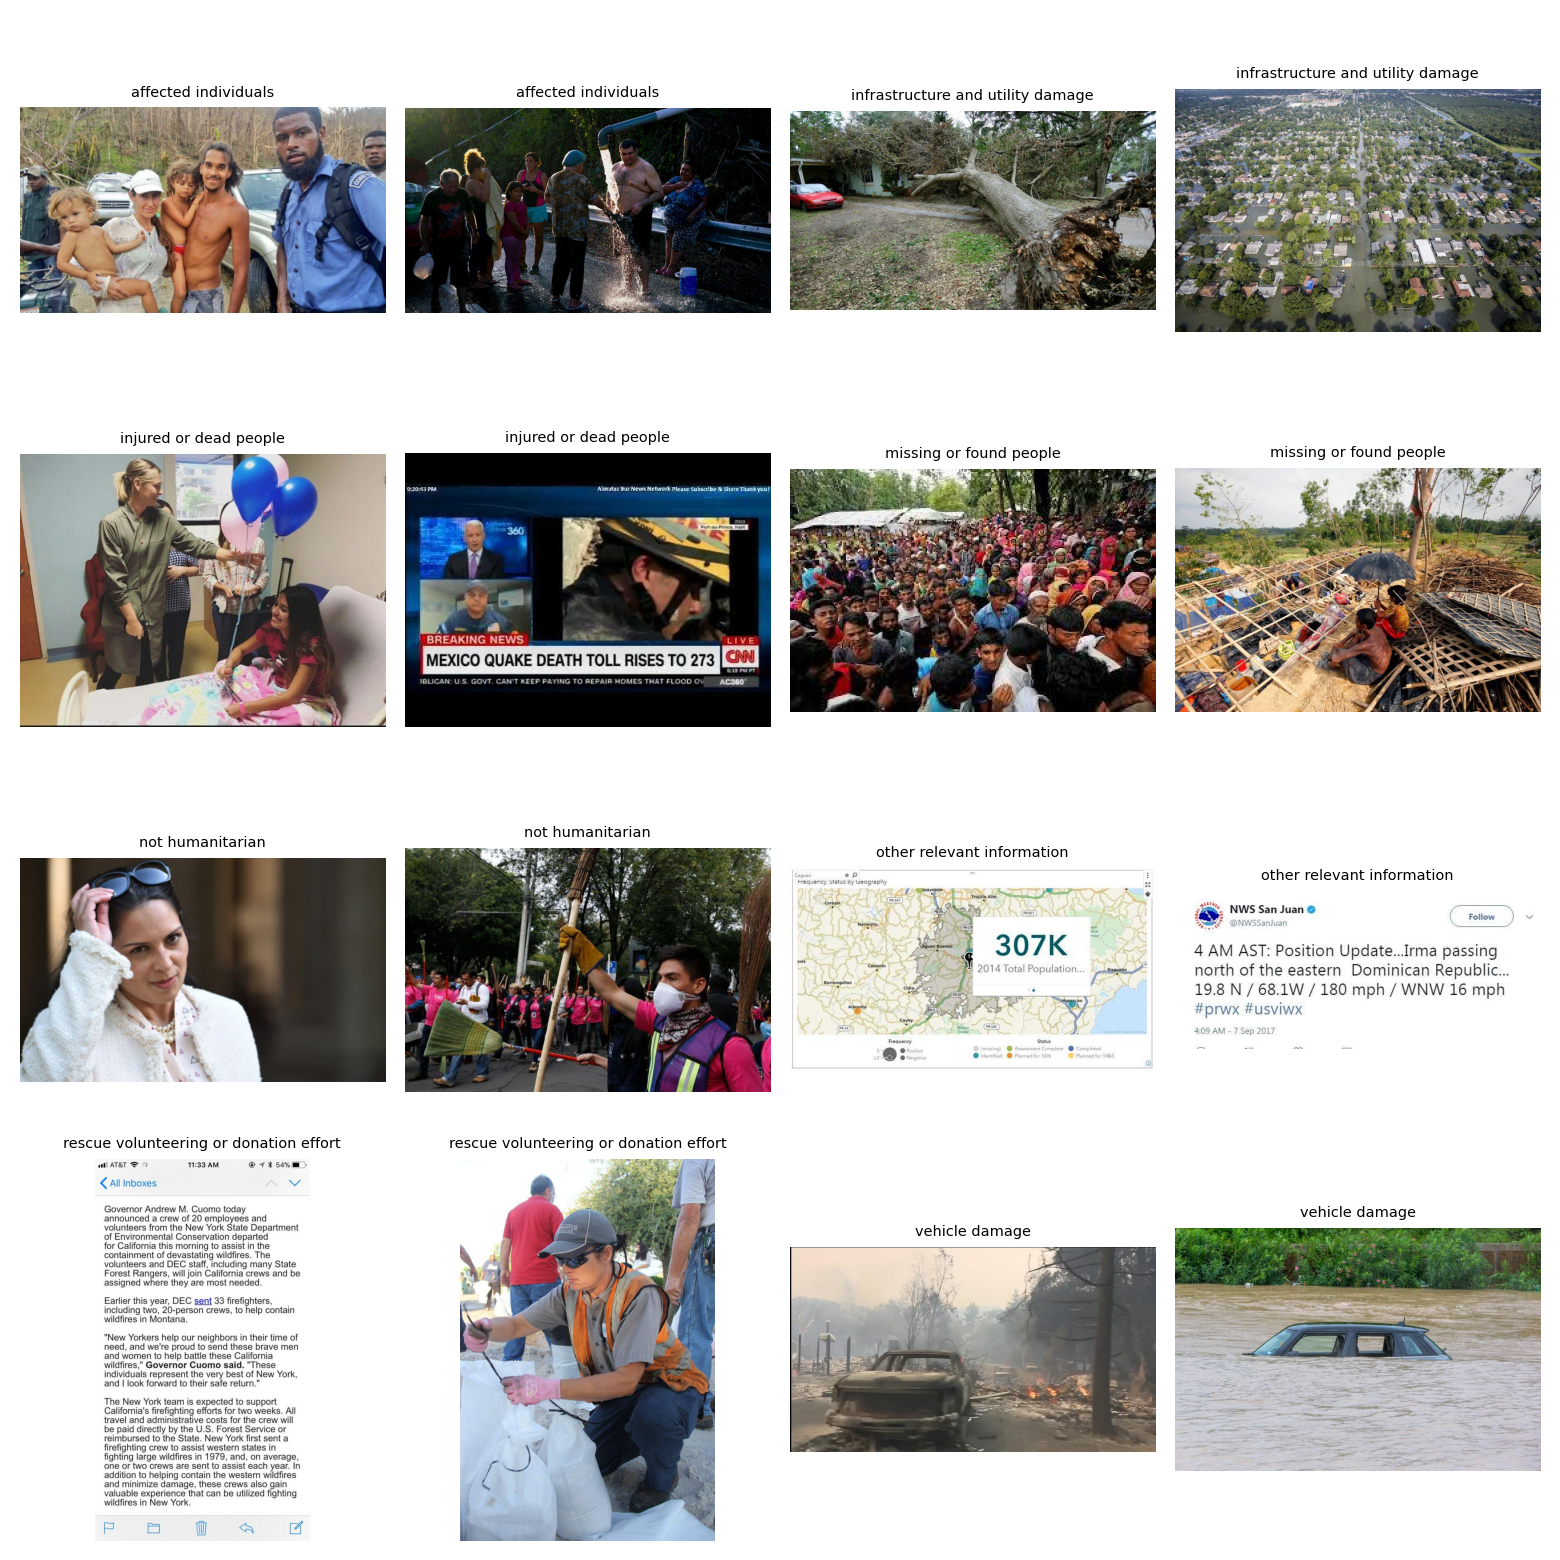
\includegraphics[width=0.92\textwidth]{image_gallery_seeded.png}
\caption{Hai ảnh train cho mỗi lớp trong tám lớp humanitarian, lấy mẫu xác định
bằng seed 42 (\emph{không} chọn tay theo ảnh ``đẹp''), nên gallery không bị thiên
lệch chủ quan.}
\end{figure}

\subsection{Lý do giữ CLIP cố định}

Giữ CLIP cố định phù hợp với phạm vi dự án vì:

\begin{itemize}[leftmargin=*]
  \item mục tiêu học phần là so sánh các thuật toán phân lớp và xây dựng DSS,
        không phải thiết kế mạng sâu;
  \item 13.608 mẫu train và các lớp hiếm rất nhỏ làm fine-tuning toàn mạng có
        nguy cơ overfit;
  \item embedding được tính một lần, sau đó cùng một không gian đặc trưng được
        dùng để so sánh công bằng sáu classifier;
  \item chi phí huấn luyện và triển khai thấp hơn, kết quả dễ tái lập hơn.
\end{itemize}

Đánh đổi là đặc trưng không được điều chỉnh riêng cho ảnh thảm họa. Kết quả của
nhánh ảnh vì vậy phải được hiểu là ``classifier trên đặc trưng CLIP cố định'',
không phải thành tích của một CLIP đã được huấn luyện cho CrisisMMD.

\section{Tổng hợp đặc trưng đầu vào mô hình}

\begin{table}[H]\centering
\caption{Đặc trưng được tạo và nơi chúng được sử dụng.}
\begin{tabularx}{\textwidth}{p{2.4cm}p{3.3cm}p{2.4cm}X}
\toprule
\textbf{Nguồn} & \textbf{Biểu diễn} & \textbf{Kích thước} & \textbf{Vai trò}\\
\midrule
Tweet & TF--IDF word 1--2 gram & 2.000, vector thưa &
Đầu vào sáu classifier văn bản cho hai task.\\
Ảnh & CLIP ViT-B/32 frozen embedding & 512, vector đặc &
Đầu vào sáu classifier ảnh cho hai task.\\
Xác suất mô hình & Vector xác suất đã căn lớp & 2 hoặc 8 &
Đầu vào Late Fusion và conflict score.\\
Từ khóa nghiệp vụ & Cờ xuất hiện trong tweet đã làm sạch & một số cờ nhị phân &
Tín hiệu bổ sung cho Risk Score, không dùng để thay đổi ground truth.\\
\bottomrule
\end{tabularx}
\end{table}

Như vậy, feature engineering của dự án không phải là một bước trang trí trước
mô hình. Nó quyết định loại thông tin mà classifier có thể nhìn thấy, chi phí
tính toán, nguy cơ rò rỉ và khả năng giải thích. Chương tiếp theo sử dụng chính
các biểu diễn này để phân tích cấu trúc dữ liệu trước khi huấn luyện.

\chapter{Phân tích khám phá dữ liệu}
\label{chap:eda}

\section{Mục đích và nguyên tắc EDA}

Exploratory Data Analysis (EDA) là quá trình dùng thống kê mô tả và trực quan
để hiểu cấu trúc dữ liệu trước khi xây mô hình. EDA không chỉ nhằm tạo biểu đồ;
nó phải trả lời các câu hỏi có ảnh hưởng tới thiết kế:

\begin{itemize}[leftmargin=*]
  \item nhãn có mất cân bằng hay không;
  \item phân bố có thay đổi giữa các sự kiện hay không;
  \item văn bản và ảnh có chứa tín hiệu quan sát được nào;
  \item có cấu trúc cụm hoặc luật đồng xuất hiện nào;
  \item hai phương thức thường đồng thuận hay mâu thuẫn;
  \item các quan sát trên dẫn tới quyết định kỹ thuật nào.
\end{itemize}

EDA phục vụ lựa chọn phương pháp chỉ sử dụng \textbf{13.608 mẫu train}. Nếu xem
phân bố nhãn hoặc pattern của test rồi điều chỉnh model, test sẽ tham gia gián
tiếp vào thiết kế. Kiểm kê file và kiểm tra duplicate được phép bao phủ toàn
corpus vì đó là kiểm soát tính toàn vẹn đầu vào, không phải tìm pattern để tối
ưu model.

\section{Phân bố nhãn và hệ quả}

\begin{figure}[H]\centering
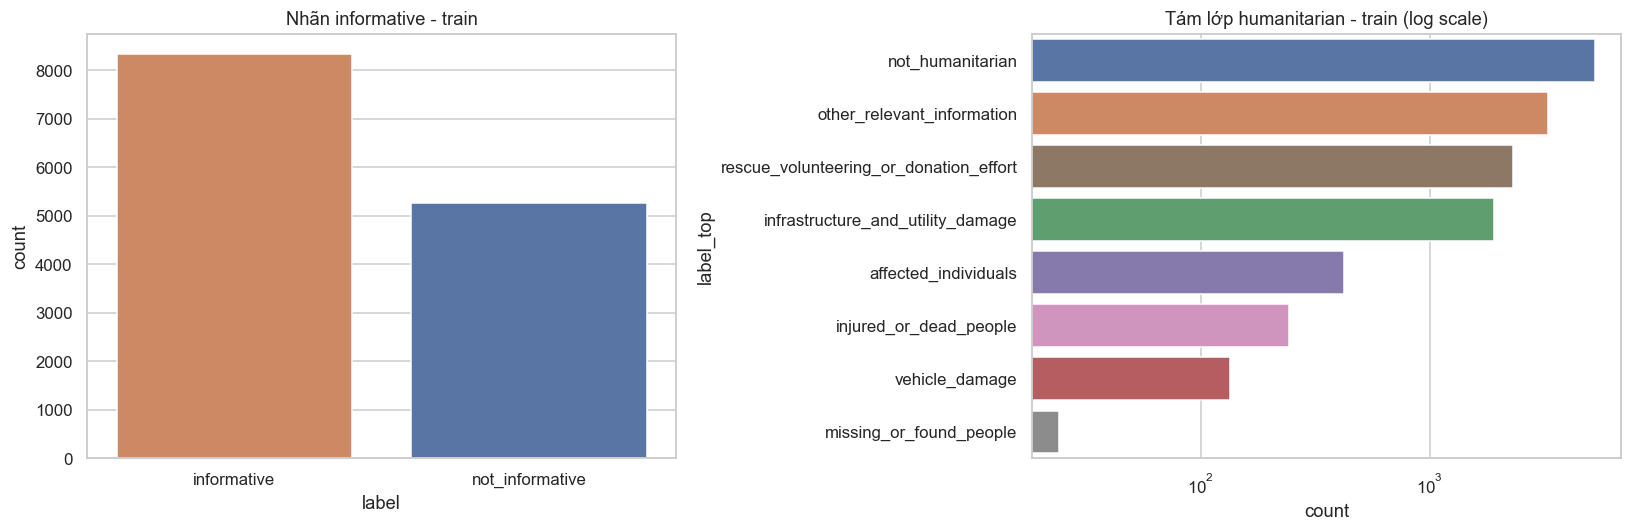
\includegraphics[width=0.92\textwidth]{label_distribution.png}
\caption{Phân bố informative và humanitarian trên train.}
\end{figure}

Informative chiếm 61,27\% train. Đây là mức lệch vừa phải nhưng đủ làm
always-informative có Recall và F2 cao. Ở task humanitarian, lớp
not-humanitarian có 5.260 mẫu trong khi missing/found chỉ có 24 mẫu, chênh
\textbf{219:1}. Ba hệ quả trực tiếp là:

\begin{enumerate}[leftmargin=*]
  \item không chọn model chỉ bằng Accuracy;
  \item sử dụng class weight khi thuật toán hỗ trợ;
  \item báo cáo Macro-F1, confusion matrix và F1 theo lớp.
\end{enumerate}

Từ phân bố không thể kết luận lớp hiếm sẽ dự báo kém trong mọi trường hợp, nhưng
có thể kết luận ước lượng metric của lớp đó có độ bất định lớn và một vài dự báo
có thể làm F1 thay đổi mạnh.

\section{Khác biệt theo sự kiện}

\begin{figure}[H]\centering
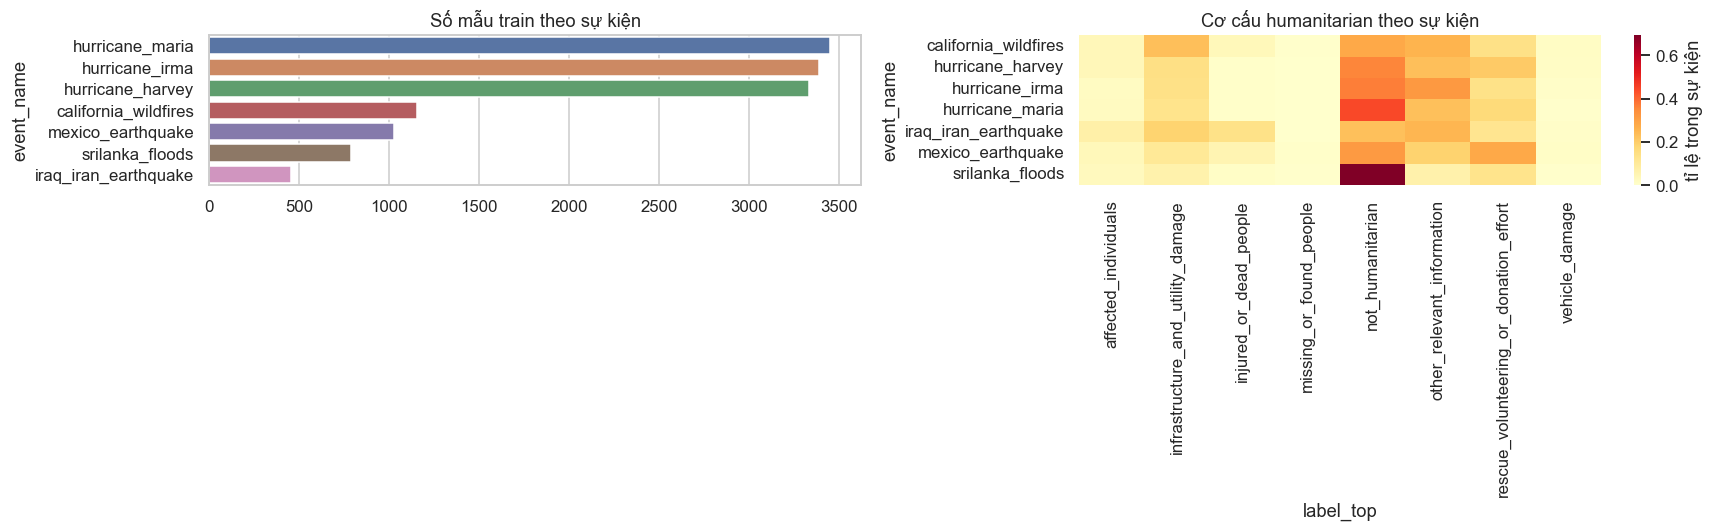
\includegraphics[width=0.92\textwidth]{event_distribution.png}
\caption{Số mẫu và cơ cấu humanitarian theo sự kiện trên train.}
\end{figure}

Sri Lanka floods có 69,29\% not-humanitarian, trong khi Iraq--Iran earthquake
chỉ 22,76\%. Mexico earthquake có 27,95\% rescue/donation; Iraq--Iran có
13,57\% injured/dead, cao hơn rõ rệt các cơn bão. Đây là
\textit{distribution shift theo sự kiện}: quan hệ giữa event và tỷ lệ nhãn
không đồng nhất.

EDA chưa chứng minh model sẽ thất bại trên event mới, vì tất cả event vẫn xuất
hiện trong train/dev/test. Tuy nhiên, nó chỉ ra rằng metric gộp có thể che khác
biệt từng thảm họa. Vì vậy dashboard có bộ lọc event và phần đánh giá sau này
báo cáo độ ổn định theo event. Một đánh giá nghiêm ngặt hơn trong tương lai là
\emph{leave-one-event-out}: giữ toàn bộ một thảm họa ngoài train
(Hình~\ref{fig:loeo}). Cách chia chính thức hiện tại cho mỗi event xuất hiện ở
cả ba split, nên mô hình luôn ``đã thấy'' kiểu dữ liệu của mọi sự kiện -- một
điều kiện dễ hơn thực tế triển khai.

\begin{figure}[H]
\centering
\begin{tikzpicture}[font=\scriptsize,
  ev/.style={draw,minimum width=0.7cm,minimum height=0.5cm,inner sep=0pt},
  tr/.style={ev,fill=HUSTBlue!25},
  te/.style={ev,fill=HUSTRed!35}]
% official split
\node[font=\small\bfseries] at (-2.3,0.6) {Chia chính thức};
\foreach \e/\x in {E1/0,E2/0.75,E3/1.5,E4/2.25,E5/3.0}{
  \node[tr] at (\x,0.85) {}; \node[tr] at (\x,0.35) {}; \node[te] at (\x,-0.15) {};
  \node[font=\tiny] at (\x+0.25,1.2) {\e};
}
\node[font=\tiny,left] at (-0.45,0.85) {train};
\node[font=\tiny,left] at (-0.45,0.35) {dev};
\node[font=\tiny,left] at (-0.45,-0.15) {test};
% leave one event out
\node[font=\small\bfseries] at (-2.3,-1.3) {Leave-one-event-out};
\foreach \e/\x in {E1/0,E2/0.75,E3/1.5,E4/2.25}{
  \node[tr] at (\x,-1.05) {};
}
\node[te] at (3.0,-1.05) {};
\node[font=\tiny] at (3.0,-0.65) {E5 (giữ ngoài)};
\node[font=\tiny,left] at (-0.45,-1.05) {train};
\end{tikzpicture}
\caption{Chia chính thức: mọi sự kiện có mặt ở cả train/dev/test. Leave-one-event-out:
toàn bộ một sự kiện bị giữ ngoài train để đo domain shift thật.}
\label{fig:loeo}
\end{figure}

\section{Khám phá văn bản}

Phần này không nhảy thẳng vào con số. Quy trình EDA văn bản đi theo bảy bước để
mỗi biểu đồ trả lời một câu hỏi cụ thể: (1) đặt câu hỏi (độ dài có phân biệt được
nhãn không?); (2) tạo biến độ dài ký tự và số token; (3) phân nhóm theo nhãn và
sự kiện; (4) so sánh phân bố; (5) xem top token nổi bật; (6) kiểm tra nhiễu còn
sót; (7) rút kết luận có giới hạn. Cần phân biệt rõ \emph{thống kê mô tả} (dữ
liệu trông thế nào) với \emph{bằng chứng dự báo} (đặc trưng có giúp phân loại
không) -- EDA chỉ cho cái thứ nhất.

Áp dụng bước (2)--(4): tweet có trung bình 117,48 ký tự và 11,72 từ sau làm sạch.
Số từ trung bình của informative là 11,75, gần như bằng 11,68 của not-informative.

\begin{figure}[H]\centering
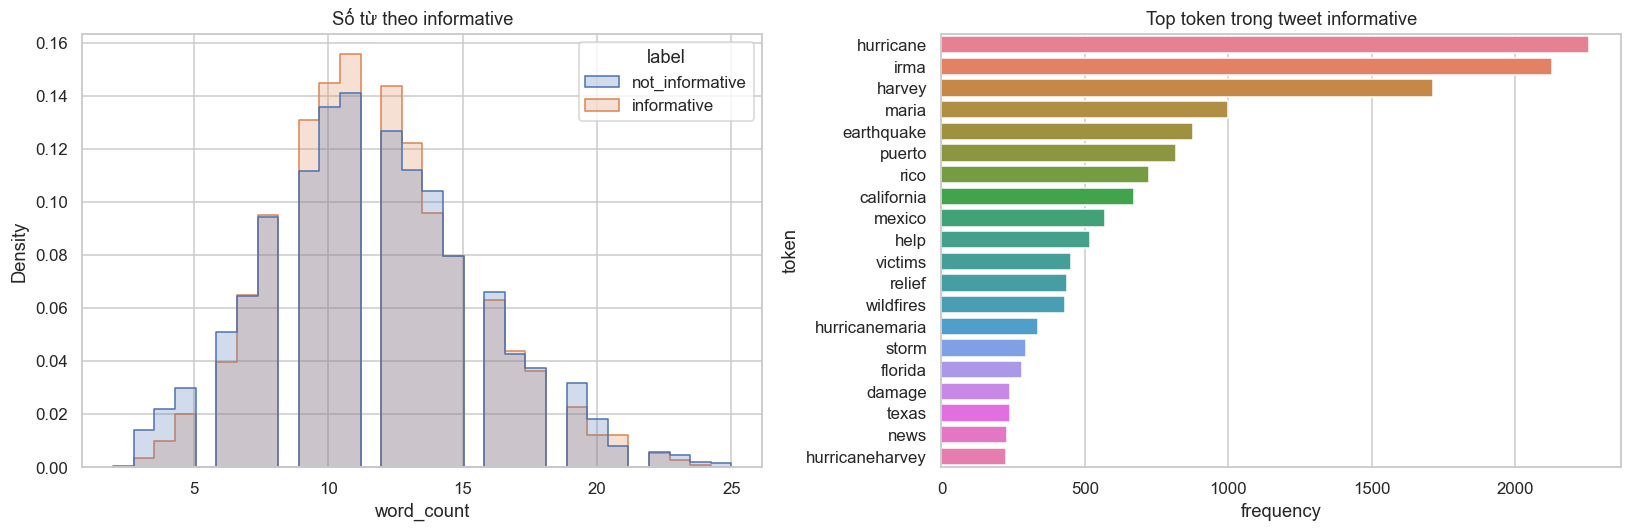
\includegraphics[width=0.92\textwidth]{text_length_distribution.png}
\caption{Phân bố độ dài và token nổi bật trên train.}
\end{figure}

Sự gần nhau của độ dài cho thấy một rule kiểu ``tweet dài thì informative''
không có cơ sở. Nội dung từ và cụm từ mới là tín hiệu phù hợp cho TF--IDF. Các
token nổi bật còn phản ánh tên địa điểm, cứu trợ, thiệt hại và bối cảnh sự kiện;
vì thế khi clustering theo chủ đề, dự án loại thêm tên event và token nền tảng
như \code{rt}, \code{amp}, \code{http} để tránh cụm chỉ tái hiện nguồn dữ liệu.

\section{K-Means cho khám phá chủ đề}

\subsection{Khái niệm và hàm mục tiêu}

Clustering là học không giám sát: thuật toán không nhìn nhãn humanitarian mà
nhóm các điểm giống nhau. K-Means tìm \(K\) tâm cụm
\(\boldsymbol{\mu}_1,\ldots,\boldsymbol{\mu}_K\) để tối thiểu hóa tổng bình
phương khoảng cách trong cụm:

\[
J=\sum_{i=1}^{n}
\left\|\mathbf{x}_i-\boldsymbol{\mu}_{c_i}\right\|_2^2.
\]

Thuật toán lặp hai bước (Hình~\ref{fig:kmeans-iter}): gán mỗi điểm vào tâm gần
nhất, rồi cập nhật tâm bằng trung bình các điểm được gán; lặp tới khi tâm không
đổi. K-Means nhanh và dễ đọc top term từ centroid, nhưng phải chọn \(K\), nhạy
với khởi tạo và giả định cụm gần \emph{dạng cầu} trong không gian khoảng cách
\cite{macqueen1967}. Giả định dạng cầu này yếu khi không gian là TF--IDF nhiều
nghìn chiều và thưa, một lý do khiến silhouette dưới đây rất thấp.

\begin{figure}[H]
\centering
\begin{tikzpicture}[font=\scriptsize,scale=0.9,
  pt/.style={circle,fill=black!55,inner sep=1.1pt},
  c1/.style={star,star points=5,fill=HUSTBlue,inner sep=1.6pt},
  c2/.style={star,star points=5,fill=HUSTRed,inner sep=1.6pt}]
% Step 1: assign
\begin{scope}
  \node[font=\small\bfseries] at (1,2.3) {1. Gán điểm vào tâm gần nhất};
  \foreach \x/\y in {0.2/0.4,0.5/0.9,0.9/0.5,0.4/1.3}{\node[pt,HUSTBlue!70,fill=HUSTBlue!50] at (\x,\y){};}
  \foreach \x/\y in {1.6/1.5,1.9/1.0,2.1/1.7,1.7/0.9}{\node[pt,HUSTRed!70,fill=HUSTRed!50] at (\x,\y){};}
  \node[c1] at (0.5,0.8){}; \node[c2] at (1.8,1.3){};
\end{scope}
% Step 2: update
\begin{scope}[xshift=4.2cm]
  \node[font=\small\bfseries] at (1,2.3) {2. Dịch tâm về trung bình cụm};
  \foreach \x/\y in {0.2/0.4,0.5/0.9,0.9/0.5,0.4/1.3}{\node[pt,fill=HUSTBlue!50] at (\x,\y){};}
  \foreach \x/\y in {1.6/1.5,1.9/1.0,2.1/1.7,1.7/0.9}{\node[pt,fill=HUSTRed!50] at (\x,\y){};}
  \node[c1] at (0.5,0.78){}; \node[c2] at (1.83,1.28){};
  \draw[-{Latex[length=1.5mm]},HUSTBlue,thick] (0.5,0.8)--(0.5,0.78);
  \draw[-{Latex[length=1.5mm]},HUSTRed,thick] (1.8,1.3)--(1.83,1.28);
\end{scope}
\end{tikzpicture}
\caption{Một vòng lặp K-Means trên ví dụ 2D: gán điểm theo tâm gần nhất rồi cập
nhật tâm. Ngôi sao là centroid.}
\label{fig:kmeans-iter}
\end{figure}

Dự án dùng TF--IDF tối đa 2.000 unigram/bigram, \code{min\_df=3}, mười lần
khởi tạo và random seed 42. Sweep \(K=2,\ldots,12\) được thực hiện trên cùng
một mẫu 8.000 dòng train để các giá trị so sánh được.

\subsection{Silhouette và kết quả}

Silhouette của điểm \(i\) là:

\[
s(i)=\frac{b(i)-a(i)}{\max\{a(i),b(i)\}},
\]

trong đó \(a(i)\) là khoảng cách trung bình tới điểm cùng cụm và \(b(i)\) là
khoảng cách trung bình nhỏ nhất tới một cụm khác. Giá trị gần 1 cho thấy điểm
nằm gọn trong cụm; gần 0 cho thấy các cụm chồng lấn; âm cho thấy có thể gán sai.

\begin{figure}[H]\centering
\begin{subfigure}{0.48\textwidth}
  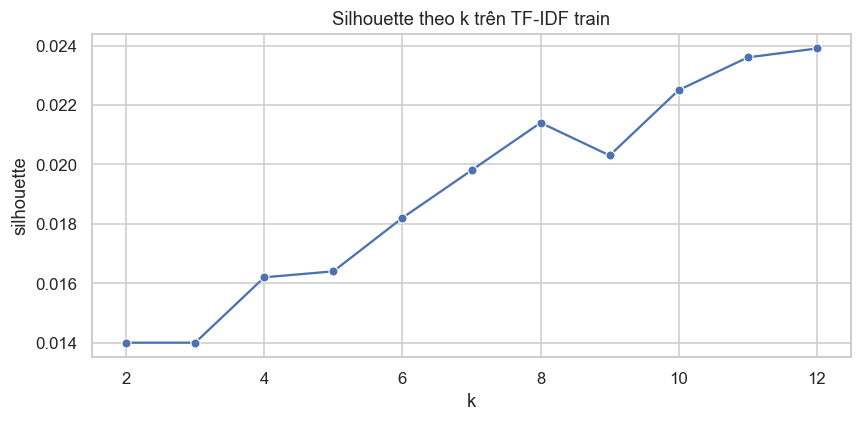
\includegraphics[width=\textwidth]{kmeans_silhouette_sweep.png}
  \caption{Silhouette với \(K=2,\ldots,12\).}
\end{subfigure}
\begin{subfigure}{0.48\textwidth}
  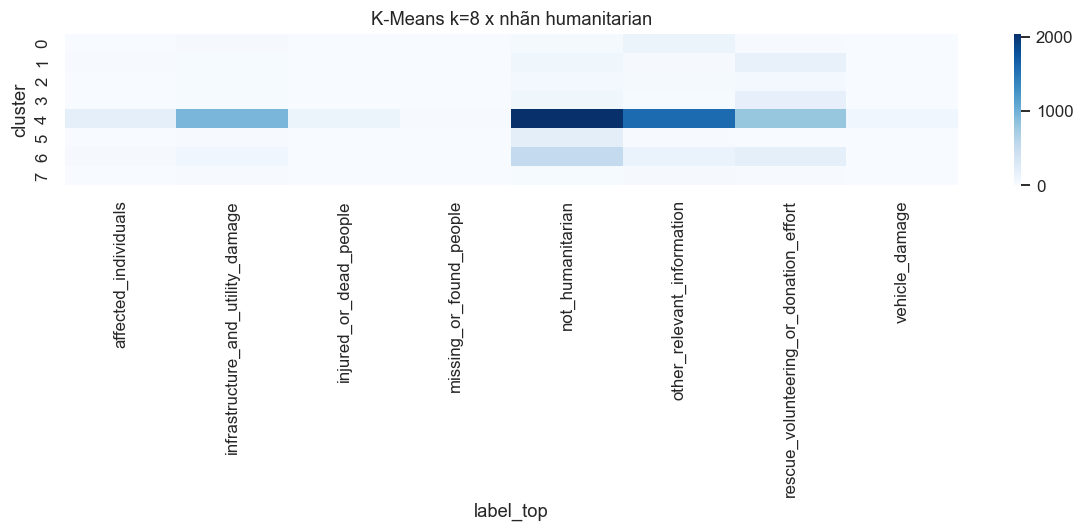
\includegraphics[width=\textwidth]{kmeans_clusters.png}
  \caption{Crosstab \(K=8\) với nhãn thật.}
\end{subfigure}
\caption{Phân cụm TF--IDF trên train.}
\end{figure}

Silhouette chỉ khoảng 0,014--0,024 và tăng nhẹ tới biên khảo sát, không có điểm
gãy rõ. Với \(K=8\), silhouette là 0,021. \(K=8\) được giữ để đối chiếu với
taxonomy tám lớp, \textbf{không phải} vì dữ liệu chứng minh tám cụm là tối ưu.

Top term cho thấy một số chủ đề có nghĩa như storm/surge, relief effort,
help victims, Puerto Rico/power và rescue. Tuy nhiên, mỗi cụm vẫn chứa nhiều
nhãn humanitarian. Kết luận hợp lệ là K-Means hữu ích để duyệt chủ đề và phát
hiện nhóm nội dung; nó không đủ ổn định để thay classifier hoặc routing.

\section{Apriori và luật kết hợp}

\subsection{Từ tweet thành transaction}

Association analysis tìm các item thường xuất hiện cùng nhau. Mỗi tweet được
chuyển thành một ``giỏ'' (transaction) gồm từ khóa khủng hoảng và hashtag. Ví dụ
cụ thể: tweet ``\#iran \#earthquake rescue teams searching'' sau khi tách trở
thành giỏ \(\{\#iran, \#earthquake, rescue\}\), rồi được biểu diễn thành một hàng
one-hot (giá trị 1 ở các cột item có mặt, 0 ở các cột còn lại):

\begin{table}[H]\centering\small
\caption{Một tweet biến thành transaction one-hot.}
\begin{tabular}{lccccc}
\toprule
& \texttt{\#iran} & \texttt{\#earthquake} & \texttt{rescue} & \texttt{flood} & \texttt{\dots}\\
\midrule
transaction & 1 & 1 & 1 & 0 & \dots\\
\bottomrule
\end{tabular}
\end{table}

Chỉ transaction có \emph{ít nhất hai item} được giữ, vì một luật cần cả tiền đề
và kết quả. Nếu một từ đã xuất hiện dưới dạng hashtag, phiên bản không có dấu
\# bị bỏ để tránh luật hiển nhiên như
\(\{\#earthquake\}\Rightarrow\{earthquake\}\). Một điểm dễ nhầm:
\textbf{mẫu số của support là số transaction đã giữ}, không phải toàn bộ 13.608
tweet train.

Apriori dựa trên tính chất: nếu một itemset không đủ phổ biến, mọi superset của
nó cũng không thể đủ phổ biến. Nhờ vậy thuật toán loại sớm nhiều ứng viên
\cite{agrawal1994}. Ba đại lượng chính là:

\[
\operatorname{support}(A\Rightarrow B)=P(A\cup B),
\]
\[
\operatorname{confidence}(A\Rightarrow B)=P(B\mid A)
=\frac{P(A\cup B)}{P(A)},
\]
\[
\operatorname{lift}(A\Rightarrow B)
=\frac{P(A\cup B)}{P(A)P(B)}.
\]

Lift bằng 1 tương ứng đồng xuất hiện như kỳ vọng nếu độc lập; lớn hơn 1 cho thấy
liên kết dương. Support trong phân tích này được tính trên tập transaction đã
giữ, không phải toàn bộ 13.608 tweet. Ngưỡng dùng là support 0,005 và confidence
0,25; 20 luật lift cao nhất được lưu.

\subsection{Kết quả và cách diễn giải}

\begin{table}[H]\centering\small
\caption{Một số luật Apriori trên train.}
\begin{tabular}{llrrr}
\toprule
\textbf{Tiền đề} & \textbf{Kết quả} & \textbf{Support} & \textbf{Confidence} & \textbf{Lift}\\
\midrule
\code{\#floodsl} & \code{\#lka} & .010 & .539 & 40.013\\
\code{\#iraq} & \code{\#iran} & .006 & .659 & 25.672\\
\code{\#wildfires} & \code{\#california} & .007 & .508 & 25.541\\
\code{\#iran} & \code{\#earthquake} & .018 & .717 & 18.507\\
\code{\#puertorico} & \code{\#hurricanemaria} & .025 & .627 & 7.045\\
\bottomrule
\end{tabular}
\end{table}

Đọc một dòng cụ thể: luật \(\{\#iran\}\Rightarrow\{\#earthquake\}\) có
support \(0{,}018\) (1,8\% giỏ chứa cả hai), confidence \(0{,}717\) (trong các
giỏ có \texttt{\#iran}, 71,7\% cũng có \texttt{\#earthquake}) và lift \(18{,}5\)
(cặp này đi cùng nhau cao gấp khoảng 18,5 lần so với khi hai hashtag độc lập).

Các luật chủ yếu nối địa danh với sự kiện, phù hợp cho filter và drill-down.
Lift cao không có nghĩa tiền đề gây ra kết quả; nó cũng có thể cao vì hai hashtag
cùng được dùng trong một chiến dịch truyền thông nhỏ. Association rules vì vậy
không dùng để dự báo Priority hay thay classifier.

\section{EDA ảnh và không gian embedding}

Kiểm kê toàn corpus xác nhận 18.082 ảnh annotation hợp lệ, nhiều kích thước và
mode màu; toàn bộ được chuyển RGB trước CLIP. Gallery theo lớp được lấy từ train
để kiểm tra trực quan rằng dữ liệu là ảnh thảm họa thật, không phải ô màu hay
placeholder.

Gallery theo lớp (lấy mẫu xác định bằng seed) đã trình bày ở
Chương~\ref{chap:dulieu}; ở đây tập trung vào \emph{không gian embedding}.

\subsection{PCA: vì sao 512 chiều khó nhìn}

Embedding CLIP đã có sẵn 512 chiều. Vì vậy để trực quan hóa phải \emph{giảm}
chiều, không phải ``tăng chiều''. PCA (Principal Component Analysis) tìm các trục
giữ nhiều phương sai nhất rồi chiếu dữ liệu xuống vài trục đó. Trên 13.608
embedding train, kết quả định lượng cho thấy không gian rất ``trải'':

\begin{itemize}[leftmargin=*]
  \item thành phần chính thứ nhất (PC1) chỉ giữ \textbf{7,5\%} phương sai, PC2
        giữ \textbf{4,8\%}; hai trục đầu cộng lại chỉ \textbf{12,4\%};
  \item cần tới \textbf{32} thành phần mới đạt 50\% phương sai tích lũy.
\end{itemize}

Con số này giải thích vì sao một hình 2D bất kỳ (PCA hay t-SNE) chỉ thấy một
lát rất mỏng của thông tin, và vì sao các lớp trông chồng lấn dù classifier vẫn
phân biệt được trên đủ 512 chiều.

\begin{figure}[H]\centering
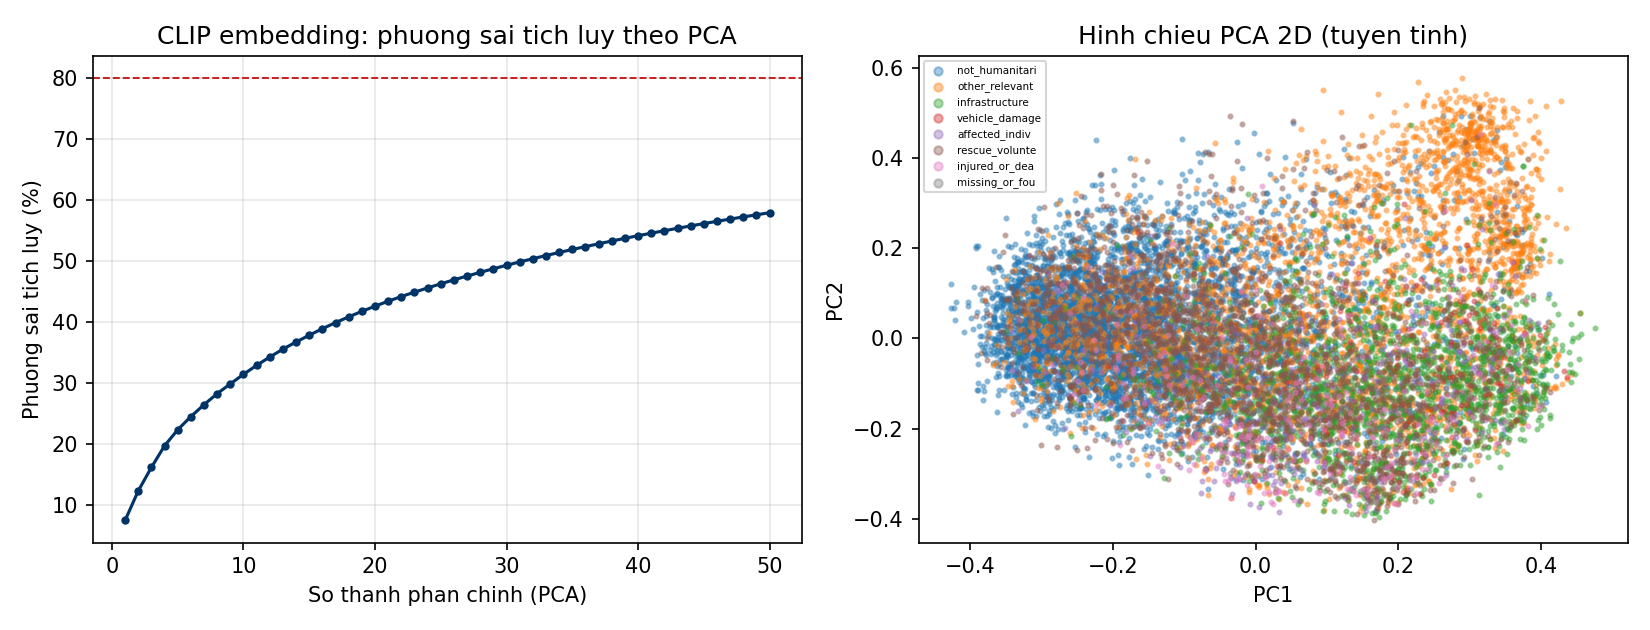
\includegraphics[width=\textwidth]{pca_clip.png}
\caption{Trái: phương sai tích lũy theo số thành phần PCA (đường ngang 80\% chưa
đạt trong 50 thành phần). Phải: hình chiếu PCA 2D tuyến tính của embedding train,
tô màu theo nhãn -- các lớp chồng lấn vì 2 trục chỉ giữ 12,4\% phương sai.}
\label{fig:pca-clip}
\end{figure}

t-SNE là phương pháp giảm chiều phi tuyến, cố gắng bảo toàn lân cận cục bộ khi
chiếu vector 512 chiều xuống hai chiều \cite{maaten2008}. Khác PCA tuyến tính,
t-SNE giữ \emph{lân cận cục bộ} nhưng \emph{không} bảo toàn khoảng cách toàn cục,
nên không dùng để chấm điểm mô hình. Hình t-SNE được tạo từ 3.000 embedding
train, perplexity 30, khởi tạo PCA và seed 42.

\begin{figure}[H]\centering
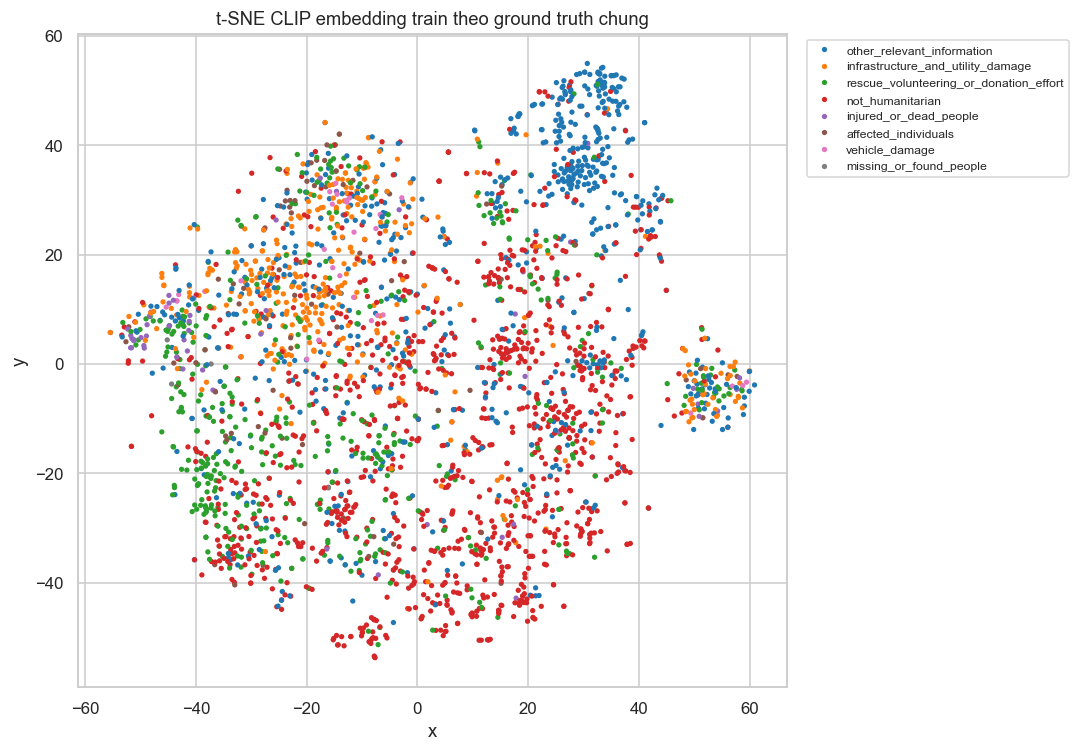
\includegraphics[width=0.82\textwidth]{tsne_clip.png}
\caption{t-SNE của CLIP embedding train, tô màu theo ground truth chung.}
\end{figure}

Một số vùng cục bộ xuất hiện nhưng các lớp chồng lấn mạnh. t-SNE có thể thay đổi
theo tham số và làm biến dạng khoảng cách toàn cục, nên hình này không chứng minh
khả năng phân lớp. Giá trị của CLIP phải được xác nhận bằng dev/test ở Chương 5.

\section{Bất đồng đa phương thức}

\begin{figure}[H]\centering
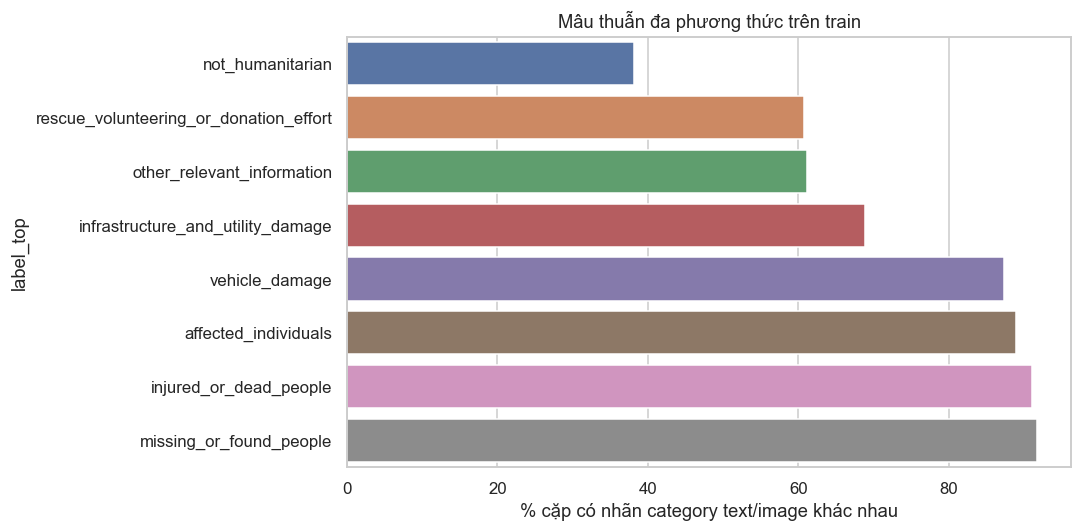
\includegraphics[width=0.86\textwidth]{multimodal_conflict.png}
\caption{Tỷ lệ nhãn category text và image bất đồng trên train.}
\end{figure}

55,0\% mẫu train có nhãn category text và ảnh khác nhau. Theo từng lớp, tỷ lệ
bất đồng là 91,7\% ở missing/found, 91,0\% ở injured/dead, 88,9\% ở affected
và 87,3\% ở vehicle damage. Not-humanitarian thấp hơn nhưng vẫn đạt 38,2\%.

Các con số không chứng minh text đúng và ảnh sai, vì nhãn riêng chỉ phản ánh
nội dung nhìn thấy ở từng phương thức. Một tweet có thể nhắc người mất tích
nhưng dùng ảnh phong cảnh, hoặc ảnh có thiệt hại mà câu chữ chỉ nêu địa danh.
Suy luận hợp lệ là hai phương thức mang bằng chứng không đồng nhất. Vì vậy:

\begin{enumerate}[leftmargin=*]
  \item fusion phải được tune trên nhãn chung chính thức;
  \item không dùng phép ``nếu text khác image thì một bên sai'';
  \item conflict cao là tín hiệu yêu cầu người kiểm tra, không tự động hạ độ tin
        cậy của mọi dự báo.
\end{enumerate}

\section{Từ bằng chứng EDA đến quyết định thiết kế}

\begin{table}[H]\centering\small
\caption{Chuỗi bằng chứng, suy luận và quyết định.}
\begin{tabularx}{\textwidth}{p{3.2cm}XX}
\toprule
\textbf{Bằng chứng train} & \textbf{Suy luận có giới hạn} & \textbf{Quyết định}\\
\midrule
Mất cân bằng 219:1 & Accuracy che khuất lớp hiếm & F2, Macro-F1, class weight\\
Event profile khác nhau & Có nguy cơ domain shift & Filter và metric theo event\\
Độ dài hai lớp gần nhau & Length không đủ phân loại & TF--IDF nội dung\\
Silhouette rất thấp & Cụm không đủ ổn định cho quyết định & K-Means chỉ cho khám phá\\
Luật hashtag lift cao & Context sự kiện có cấu trúc & Drill-down phụ trợ\\
55\% modality bất đồng & Không tin tuyệt đối một nhánh & Tune fusion, Manual Review\\
Ảnh lặp xuyên split & Metric có thể lạc quan & Canonical/robust mask\\
\bottomrule
\end{tabularx}
\end{table}

EDA vì vậy có giá trị khi nó thay đổi cách đánh giá và kiến trúc. Các kết luận
trên đều dừng ở mức dữ liệu cho phép; tương quan, hình chiếu hai chiều và luật
đồng xuất hiện không được diễn giải thành quan hệ nhân quả.

\chapter{Mô hình, Late Fusion và tầng quyết định}

\section{Thiết kế thực nghiệm}
Sáu model được fit trên 13.608 train rows. Model tốt nhất, trọng số fusion và threshold
được chọn trên 2.189 dev rows leakage-safe. Test 2.169 rows chỉ dùng báo cáo cuối. Text,
ảnh và fusion cùng dự báo nhãn chính thức; modality label chỉ dùng chẩn đoán.

\section{So sánh sáu model trên dev}
\begin{table}[H]\centering\scriptsize
\caption{Text informative, chọn theo F2.}
\begin{tabular}{lrrrrr}
\toprule
\textbf{Model} & \textbf{Acc.} & \textbf{Prec.} & \textbf{Recall} & \textbf{F1} & \textbf{F2}\\
\midrule
Logistic Regression & .7085 & .7816 & .7368 & .7585 & .7453\\
Decision Tree & .6044 & .7546 & .5382 & .6283 & .5710\\
Naive Bayes & .7177 & .7265 & .8750 & .7939 & .8406\\
k-NN & .4523 & .7193 & .1941 & .3057 & .2273\\
\textbf{Linear SVM} & \textbf{.7204} & .7234 & \textbf{.8904} & \textbf{.7983} & \textbf{.8511}\\
Random Forest & .7195 & .7457 & .8324 & .7867 & .8135\\
\bottomrule
\end{tabular}
\end{table}

\begin{table}[H]\centering\scriptsize
\caption{Text humanitarian, chọn theo Macro-F1.}
\begin{tabular}{lrrrrr}
\toprule
\textbf{Model} & \textbf{Acc.} & \textbf{Macro-P} & \textbf{Macro-R} &
\textbf{Macro-F1} & \textbf{Weighted-F1}\\
\midrule
\textbf{Logistic Regression} & .4641 & .3145 & \textbf{.4095} & \textbf{.3297} & .4875\\
Decision Tree & .2810 & .2118 & .2346 & .1302 & .1747\\
Naive Bayes & \textbf{.5263} & .2677 & .2429 & .2446 & \textbf{.4982}\\
k-NN & .4079 & \textbf{.3940} & .1449 & .1195 & .2871\\
Linear SVM & .5112 & .3019 & .2697 & .2787 & .4856\\
Random Forest & .4947 & .2921 & .2571 & .2626 & .4734\\
\bottomrule
\end{tabular}
\end{table}

\begin{table}[H]\centering\scriptsize
\caption{Image informative trên CLIP, chọn theo F2.}
\begin{tabular}{lrrrrr}
\toprule
\textbf{Model} & \textbf{Acc.} & \textbf{Prec.} & \textbf{Recall} & \textbf{F1} & \textbf{F2}\\
\midrule
Logistic Regression & .7579 & .8529 & .7375 & .7910 & .7580\\
Decision Tree & .6807 & .7487 & .7316 & .7401 & .7350\\
Naive Bayes & .7177 & \textbf{.8681} & .6434 & .7390 & .6785\\
\textbf{k-NN} & .7542 & .7915 & \textbf{.8206} & \textbf{.8058} & \textbf{.8146}\\
Linear SVM & \textbf{.7593} & .8078 & .8037 & \textbf{.8058} & .8045\\
Random Forest & .7478 & .7949 & .8007 & .7978 & .7996\\
\bottomrule
\end{tabular}
\end{table}

\begin{table}[H]\centering\scriptsize
\caption{Image humanitarian trên CLIP, chọn theo Macro-F1.}
\begin{tabular}{lrrrrr}
\toprule
\textbf{Model} & \textbf{Acc.} & \textbf{Macro-P} & \textbf{Macro-R} &
\textbf{Macro-F1} & \textbf{Weighted-F1}\\
\midrule
\textbf{Logistic Regression} & .5354 & .3603 & \textbf{.4768} & \textbf{.3637} & .5653\\
Decision Tree & .4079 & .2288 & .2406 & .2323 & .4163\\
Naive Bayes & .5477 & .3462 & .4028 & .3362 & .5590\\
k-NN & .5943 & .4101 & .3530 & .3563 & .5851\\
Linear SVM & \textbf{.6190} & .4889 & .3586 & .3631 & \textbf{.5970}\\
Random Forest & .5706 & \textbf{.5433} & .2760 & .2795 & .5262\\
\bottomrule
\end{tabular}
\end{table}

k-NN thất bại trên TF--IDF thưa nhưng cạnh tranh trên embedding ảnh. SVM có F2 tốt cho
text informative. Với bài toán tám lớp, Logistic Regression không có Accuracy cao nhất
nhưng có Macro-F1 tốt nhất do cân bằng lớp hiếm tốt hơn; đây là lý do chọn metric trước
khi nhìn kết quả.

\section{Đối chứng dummy baseline}
Test leakage-safe có 62,75\% mẫu informative. Vì F2 nhấn mạnh Recall, bộ phân loại luôn
dự báo informative đã đạt F2 0,8939 dù Balanced Accuracy chỉ 0,5 và MCC bằng 0.
\begin{table}[H]\centering\small
\caption{Đối chứng informative trên test leakage-safe.}
\begin{tabular}{lrrrrrr}
\toprule
\textbf{Hệ thống} & \textbf{Acc.} & \textbf{Balanced Acc.} &
\textbf{F1} & \textbf{F2} & \textbf{MCC} & \textbf{Avg. Precision}\\
\midrule
Always informative & .6275 & .5000 & .7711 & .8939 & .0000 & .6275\\
Late Fusion & .7072 & .6136 & .8079 & .9035 & .3602 & .8921\\
\bottomrule
\end{tabular}
\end{table}

Chênh lệch F2 chỉ 0,0096. Giá trị của fusion ở task này phải được nhìn đồng thời qua
Accuracy tăng 0,0797, F1 tăng 0,0368, Balanced Accuracy và MCC dương; không dùng F2 riêng
lẻ làm headline chất lượng.

Với humanitarian, majority baseline luôn dự báo \code{not\_humanitarian}, đạt Accuracy
0,3785 nhưng Macro-F1 chỉ 0,0686. Fusion đạt Macro-F1 0,4005, cho thấy khả năng phân biệt
tám lớp vượt baseline rõ hơn nhiều.

\section{Late Fusion trên test}
Dev chọn informative text/image \(=0,70/0,30\), threshold 0,38; category dùng
\(0,55/0,45\).
\begin{table}[H]\centering\small
\caption{Informative trên test leakage-safe.}
\begin{tabular}{lrrrrrr}
\toprule
\textbf{Hệ thống} & \textbf{Threshold} & \textbf{Acc.} & \textbf{Prec.} &
\textbf{Recall} & \textbf{F1} & \textbf{F2}\\
\midrule
Text-only & .34 & .6745 & .6619 & .9838 & .7914 & .8966\\
Image-only & .20 & .6754 & .6643 & .9758 & .7905 & .8921\\
\textbf{Late Fusion} & .38 & \textbf{.7072} & \textbf{.6867} & .9809 &
\textbf{.8079} & \textbf{.9035}\\
\bottomrule
\end{tabular}
\end{table}

\begin{table}[H]\centering\small
\caption{Humanitarian trên test leakage-safe.}
\begin{tabular}{lrrr}
\toprule
\textbf{Hệ thống} & \textbf{Accuracy} & \textbf{Macro-F1} & \textbf{Weighted-F1}\\
\midrule
Text-only & .4481 & .3260 & .4693\\
Image-only & .5440 & .3646 & .5695\\
\textbf{Late Fusion} & \textbf{.5569} & \textbf{.4005} & \textbf{.5776}\\
\bottomrule
\end{tabular}
\end{table}

Fusion cải thiện Accuracy/F1 informative và Macro-F1 tám lớp. Lợi thế F2 informative so
với dummy nhỏ, trong khi lợi thế humanitarian so với majority baseline rõ hơn. Điều này
hỗ trợ giữ ảnh như bằng chứng bổ sung, nhưng không đủ để kết luận hệ thống tốt đồng đều ở
mọi lớp.

\section{Phân tích theo lớp}
\begin{table}[H]\centering\scriptsize
\caption{Late Fusion humanitarian theo lớp trên test sạch.}
\begin{tabular}{lrrrr}
\toprule
\textbf{Lớp} & \textbf{Precision} & \textbf{Recall} & \textbf{F1} & \textbf{Support}\\
\midrule
injured/dead & .2202 & .6316 & .3265 & 38\\
missing/found & .0435 & .2000 & .0714 & 5\\
rescue/donation & .5262 & .5468 & .5363 & 331\\
infrastructure & .4925 & .5305 & .5108 & 311\\
affected & .2124 & .5000 & .2982 & 82\\
vehicle damage & .1385 & .5000 & .2169 & 18\\
other relevant & .6588 & .4938 & .5645 & 563\\
not humanitarian & .7507 & .6200 & .6791 & 821\\
\bottomrule
\end{tabular}
\end{table}

Missing/found chỉ có 5 mẫu test sạch và F1 0,0714; vehicle damage có 18 mẫu và F1 0,2169.
Đây là giới hạn trọng yếu: các lớp sinh tử/hiếm chưa đủ bằng chứng để tự động hóa quyết định.

\section{Hậu kiểm robustness và độ bất định}
Canonical mask chỉ loại exact duplicate theo ảnh/text đã xuất hiện ở split trước. Sau
review từng cặp, robust mask loại thêm 137 test rows near-duplicate đã xác minh, còn
2.032 rows. Toàn bộ model, trọng số fusion và threshold được giữ nguyên; không fit, chọn
hay tune lại trên robust rows.

\begin{table}[H]\centering\small
\caption{Độ nhạy metric khi chuyển từ canonical sang robust test.}
\begin{tabular}{lrrr}
\toprule
\textbf{Metric} & \textbf{Canonical} & \textbf{Robust} & \textbf{Chênh lệch}\\
\midrule
Informative Accuracy & .7072 & .7018 & -.0055\\
Informative F1 & .8079 & .8029 & -.0050\\
Informative F2 & .9035 & .9006 & -.0029\\
Informative MCC & .3602 & .3592 & -.0010\\
Humanitarian Macro-F1 & .4005 & .3908 & -.0097\\
Humanitarian Weighted-F1 & .5776 & .5789 & +.0013\\
Manual Review F1 & .4687 & .4665 & -.0021\\
\bottomrule
\end{tabular}
\end{table}

Kết quả không phụ thuộc mạnh vào các near-duplicate đã xác nhận. Macro-F1 giảm nhiều hơn
các metric khác vì robust test chỉ còn 28 mẫu injured/dead, 4 missing/found và 15 vehicle
damage; thay đổi vài dự báo làm F1 lớp hiếm dao động rõ.

Bootstrap phân tầng 2.000 lần trên robust test cho kết quả:
\begin{table}[H]\centering\small
\caption{Khoảng tin cậy percentile 95\%, cấu hình đã khóa.}
\begin{tabular}{lrrr}
\toprule
\textbf{Đại lượng} & \textbf{Ước lượng} & \textbf{CI thấp} & \textbf{CI cao}\\
\midrule
Informative F2 & .9006 & .8938 & .9068\\
F2 gain so với always-informative & .0100 & .0032 & .0161\\
Humanitarian Macro-F1 & .3908 & .3636 & .4208\\
Macro-F1 gain so với majority & .3208 & .2936 & .3508\\
Manual Review F1 & .4665 & .4370 & .4962\\
\bottomrule
\end{tabular}
\end{table}

Paired F2 gain có CI không chứa 0 dưới giả định lấy mẫu độc lập theo hàng, nhưng độ lớn
thực tiễn chỉ khoảng 0,01. Đây không phải bằng chứng tổng quát hóa sang một thảm họa chưa
từng thấy, vì các hàng trong cùng event có thể tương quan.

\begin{figure}[H]\centering
\begin{subfigure}{0.48\textwidth}
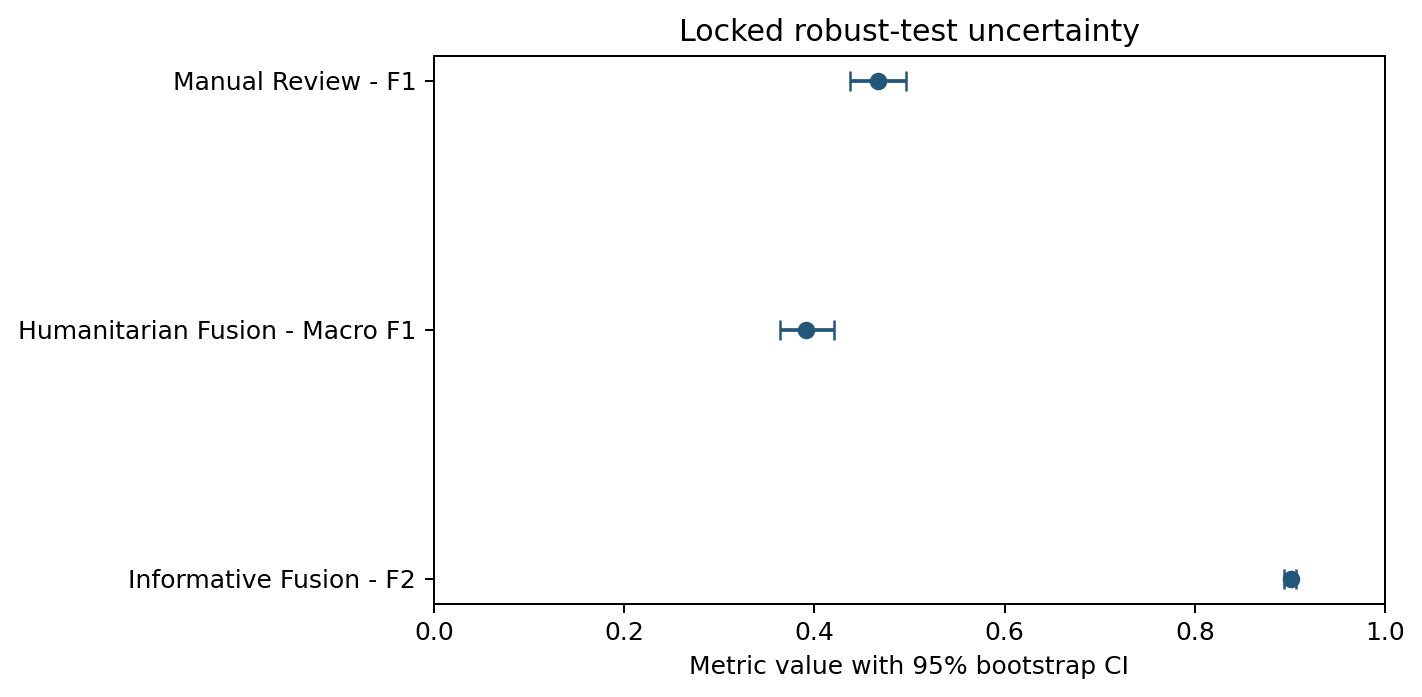
\includegraphics[width=\textwidth]{robust_bootstrap_intervals.png}
\caption{CI bootstrap trên robust test.}
\end{subfigure}
\hfill
\begin{subfigure}{0.48\textwidth}
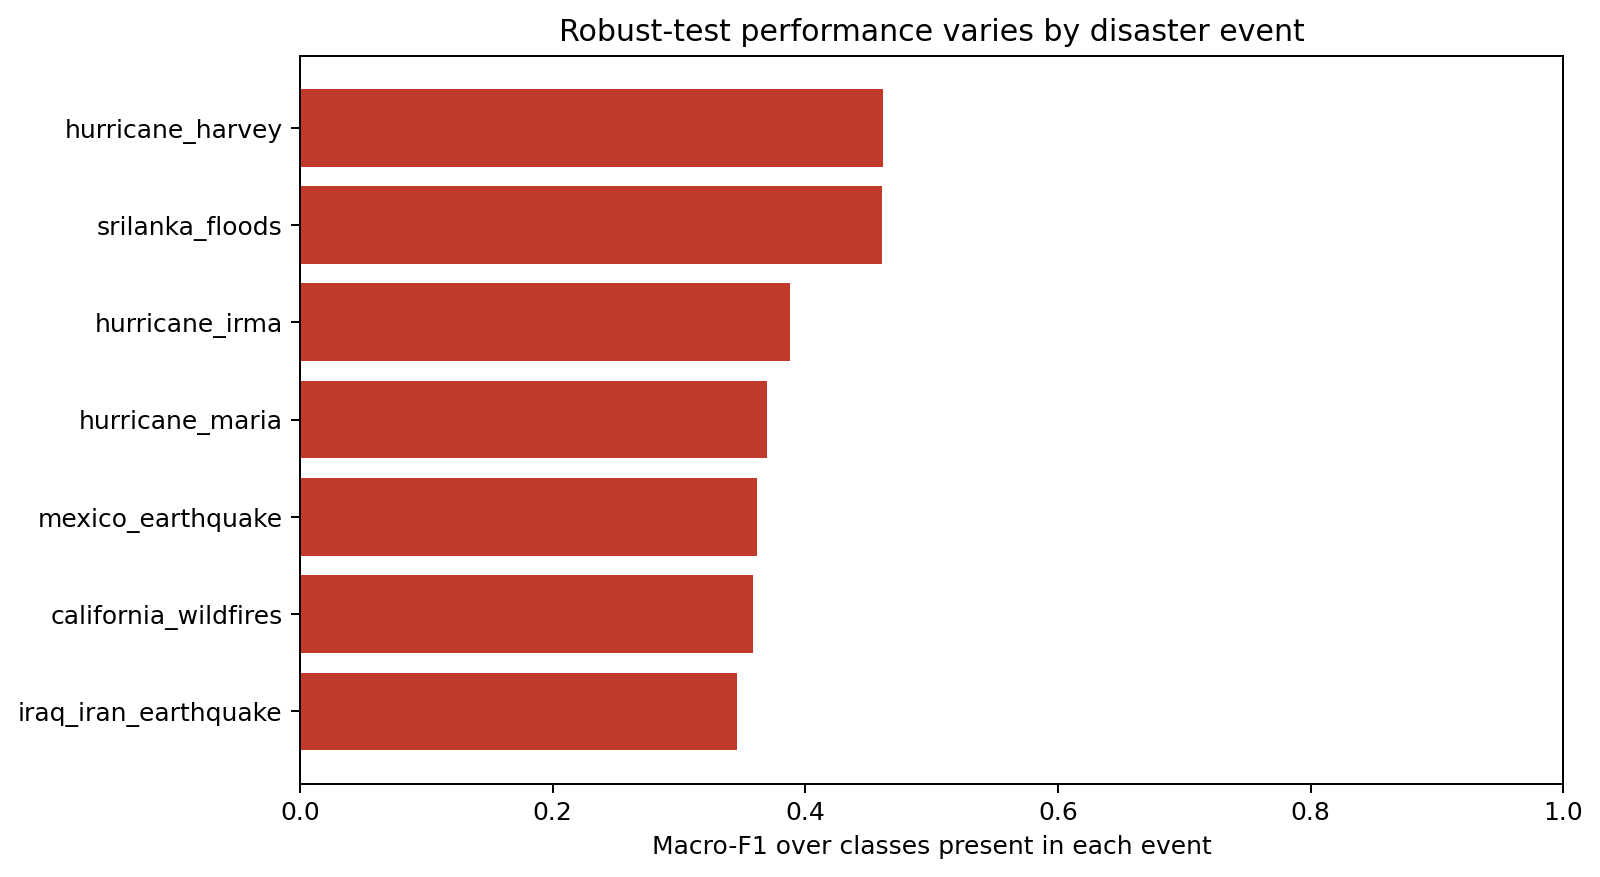
\includegraphics[width=\textwidth]{robust_event_stability.png}
\caption{Macro-F1 theo event.}
\end{subfigure}
\caption{Độ bất định tổng thể và biến động theo thảm họa.}
\end{figure}

Informative F2 theo event nằm trong khoảng 0,8377--0,9270, thấp nhất ở
\code{srilanka\_floods}. Humanitarian Macro-F1 tính trên các lớp hiện diện nằm trong
0,3458--0,4615, thấp nhất ở \code{iraq\_iran\_earthquake} chỉ có 61 rows. Ba lớp
injured/dead, missing/found và vehicle damage vẫn dưới 30 mẫu; không có lớp support đủ
lớn nào dịch F1 quá 0,05 giữa canonical và robust mask.

\section{Manual Review}
Conflict score là giá trị lớn hơn giữa chênh lệch informative và total-variation distance
của hai phân bố tám lớp. Ngưỡng 0,54 được chọn trên dev với capacity tối đa 25\%. Trên test:
review rate 25,63\%, Precision 0,7536, Recall 0,3401, F1 0,4687. Hệ thống ưu tiên xung đột
mạnh thay vì đẩy mọi trường hợp cho người.

\section{Risk Score và routing}
Risk Score là chính sách minh bạch:
\[
\begin{aligned}
\operatorname{Risk}={}&0,40S_{\mathrm{informative}}
+0,25S_{\mathrm{severity}}\\
&+0,20S_{\mathrm{keyword}}
+0,15(S_{\mathrm{severity}}\times C_{\mathrm{category}}).
\end{aligned}
\]
Confidence được nhân severity để một dự báo rất chắc chắn là \code{not\_humanitarian}
không làm tăng risk. Ngưỡng 0--39/40--69/70--100 ánh xạ Low/Medium/High. Tám category có
routing đầy đủ đến Emergency, Relief, Infrastructure, Coordination hoặc No Action.

CrisisMMD không có ground truth Priority. Vì vậy trọng số và threshold trên là giả định chính
sách, không phải optimum học được. Sensitivity trên 2.169 test rows:
\begin{table}[H]\centering\small
\caption{Độ nhạy của số lượng case theo policy threshold.}
\begin{tabular}{lrrrr}
\toprule
\textbf{Policy} & \textbf{Low max} & \textbf{Medium max} &
\textbf{Medium cases} & \textbf{High cases}\\
\midrule
Sensitive & 29 & 59 & 1.174 & 346\\
Current & 39 & 69 & 1.338 & 55\\
Strict & 49 & 79 & 968 & 2\\
\bottomrule
\end{tabular}
\end{table}

Khi conflict cao, Low được nâng lên Medium; High giữ nguyên High. Supervisor review song
song với đội phản ứng gốc, ví dụ \code{Supervisor + Emergency Team}, tránh lỗi hạ mức hoặc
chặn phản ứng khẩn cấp.

\begin{insight}[Kết luận GĐ3--GĐ4]
GĐ3 hoàn thành vì có đủ bốn bảng so sánh sáu model, dummy baseline, lựa chọn trên dev,
test sạch, fusion, robustness, confusion/per-class analysis. GĐ4 hoàn thành ở mức prototype vì routing phủ tám lớp,
Manual Review có capacity, scenario test bảo toàn High Priority và sensitivity công khai
tính phụ thuộc chính sách. Risk Score chưa được xác nhận bằng ground truth ưu tiên thực tế.
\end{insight}

\chapter{Diễn giải kết quả và khuyến nghị}

\section{Kết quả end-to-end}

Hệ thống hoàn chỉnh chuyển một cặp tweet--ảnh qua chuỗi:

\[
\text{dữ liệu}\rightarrow\text{đặc trưng}\rightarrow
\text{xác suất}\rightarrow\text{fusion}\rightarrow
\text{chính sách DSS}\rightarrow\text{hàng đợi}.
\]

Integration test sử dụng một bài đăng Hurricane Harvey về hoạt động cứu trợ.
Hệ thống dự báo đúng nhóm rescue/donation, tạo Risk Score 54,3, Priority Medium
và định tuyến Relief Team. Kiểm thử này chứng minh các module có thể phối hợp
trên một ảnh thật; nó không thay thế đánh giá thống kê trên toàn test.

Dashboard vận hành trên 2.237 dòng test để người dùng có đủ batch quan sát: 50
case High và 571 case Manual Review. Các metric khoa học chỉ tính trên 2.169
dòng canonical test; trong tập này có 49 High và 539 Manual Review. Việc tách
hai con số tránh nhầm dashboard workload với tập đánh giá đã lọc duplicate.

\section{Ý nghĩa của kết quả mô hình}

\subsection{Sàng lọc informative}

Fusion đạt F2 .9045, nhưng baseline luôn dự báo informative đã đạt .8939. Mức
tăng .0106 là nhỏ về độ lớn thực tiễn dù CI bootstrap của gain không chứa 0.
Giá trị bổ sung rõ hơn ở Accuracy (.6948 so với .6275), F1 (.8025 so với
.7711), Balanced Accuracy (.5944 so với .5000) và MCC (.3325 so với 0).

\begin{figure}[H]
\centering
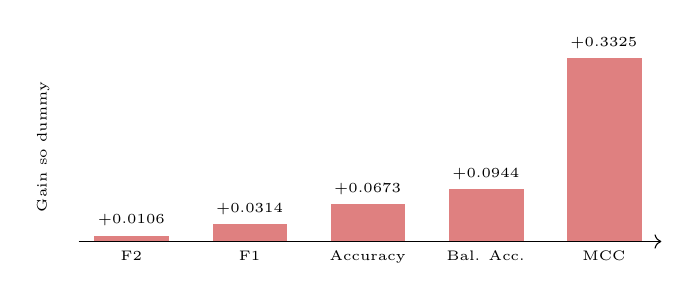
\begin{tikzpicture}[font=\scriptsize]
\def\sc{7.0}
\foreach \v/\lab/\x in {0.0106/F2/0, 0.0314/F1/1.5, 0.0673/Accuracy/3.0,
  0.0944/{Bal. Acc.}/4.5, 0.3325/MCC/6.0}{
  \fill[HUSTRed!55] (\x,0) rectangle ++(0.95,\v*\sc);
  \node[above,font=\tiny] at (\x+0.47,\v*\sc) {+\v};
  \node[below,align=center,font=\tiny] at (\x+0.47,0) {\lab};
}
\draw[->] (-0.2,0) -- (7.2,0);
\node[rotate=90,anchor=south,font=\tiny] at (-0.45,1.2) {Gain so dummy};
\end{tikzpicture}
\caption{Mức tăng của Late Fusion so với baseline always-informative theo từng
metric (canonical test). F2 gần như không nhúc nhích, nhưng các metric cân bằng
(Balanced Accuracy, MCC) tăng rõ -- đây mới là giá trị thật của fusion.}
\label{fig:informative-delta}
\end{figure}

Hình~\ref{fig:informative-delta} cho thấy ngay vì sao không được khoe F2 đơn
độc: cột F2 thấp nhất, còn MCC tăng từ 0 lên .3325 mới là bằng chứng mô hình
phân biệt hai lớp hơn hẳn dự báo hằng.

Điều này có nghĩa hệ thống phân biệt hai lớp tốt hơn dự báo hằng, nhưng ưu tiên
Recall khiến nhiều not-informative vẫn bị chuyển tiếp. Trong bối cảnh cứu trợ,
đó có thể là đánh đổi chấp nhận được ở tầng sàng lọc đầu tiên, miễn là tầng sau
có hàng đợi và con người kiểm tra. Không nên mô tả informative model là bộ lọc
chính xác cao hoặc dùng nó để tự động loại bỏ mọi bài có xác suất thấp.

\subsection{Phân loại nhu cầu humanitarian}

Humanitarian fusion đạt Macro-F1 .4005, cao hơn image-only .3646, text-only
.3260 và majority baseline .0686. Mức tăng so với baseline rõ hơn task
informative vì model thực sự phân biệt nhiều lớp thay vì chỉ tận dụng tỷ lệ
lớp dương.

Tuy nhiên, kết quả không đồng đều. F1 là .6791 ở not-humanitarian, .5645 ở
other-relevant và .5363 ở rescue/donation, nhưng chỉ .0714 ở missing/found.
Do đó hệ thống có giá trị cho tổ chức hàng đợi tổng thể, chưa đủ tin cậy để một
nhãn lớp hiếm tự kích hoạt điều động sinh tử.

\begin{figure}[H]
\centering
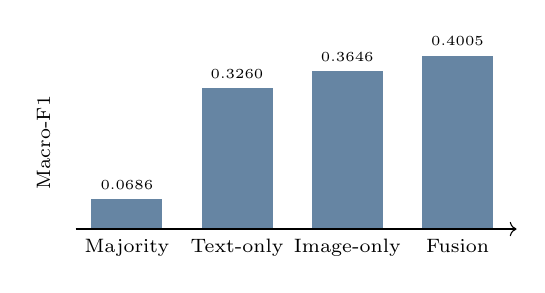
\begin{tikzpicture}[font=\scriptsize]
\def\sc{5.5}
\foreach \v/\lab/\x in {0.0686/Majority/0, 0.3260/Text-only/1.4,
  0.3646/Image-only/2.8, 0.4005/Fusion/4.2}{
  \fill[HUSTBlue!60] (\x,0) rectangle ++(0.9,\v*\sc);
  \node[above,font=\tiny] at (\x+0.45,\v*\sc) {\v};
  \node[below,align=center] at (\x+0.45,0) {\lab};
}
\draw[->] (-0.2,0) -- (5.4,0);
\node[rotate=90,anchor=south] at (-0.4,1.1) {Macro-F1};
\end{tikzpicture}
\caption{Tiến triển Macro-F1 humanitarian qua các mốc đối chứng trên canonical
test: mỗi bước thêm thông tin đều nhích lên, fusion cao nhất.}
\label{fig:results-progression}
\end{figure}

Hình~\ref{fig:results-progression} cho thấy điều mà một bảng số khó truyền tải
ngay: khoảng cách lớn nhất là từ majority lên các mô hình thật, và fusion vượt
cả hai nhánh đơn lẻ. Người đọc không cần tự trừ các con số trong bảng.

\subsection{Giá trị của nhánh ảnh}

Image-only tốt hơn text-only ở humanitarian Macro-F1 (.3646 so với .3260), và
fusion tốt hơn cả hai. Đây là bằng chứng ảnh cung cấp thông tin bổ sung. EDA lại
cho thấy nhãn text--image bất đồng cao ở lớp khẩn cấp. Hai kết quả không mâu
thuẫn: ảnh có thể hữu ích trên trung bình nhưng vẫn không khớp văn bản ở nhiều
case cụ thể.

Kết luận vận hành là giữ ảnh như một nguồn bằng chứng độc lập, không gán cho nó
vai trò ``xác nhận chân lý''. Khi hai nhánh bất đồng mạnh, hệ thống tăng nhu cầu
xác minh thay vì tự chọn một nhánh.

\section{Ý nghĩa của Manual Review}

Với giới hạn công suất dev 25\%, ngưỡng conflict 0,54 tạo review rate 24,85\%
trên canonical test. Diễn giải bằng \emph{số ca} dễ hình dung hơn tỷ lệ: trên
2.169 dòng test, hệ thống đẩy khoảng \(539\) ca vào hàng review. Precision .7532
nghĩa là trong \(539\) ca đó có khoảng \(406\) ca thực sự bất đồng theo
annotation và khoảng \(133\) ca là báo nhầm. Recall .3295 nghĩa là hệ thống chỉ
thu hồi khoảng một phần ba \emph{toàn bộ} ca bất đồng -- phần còn lại lọt qua.
Đây là một đánh đổi công suất: muốn bắt nhiều hơn phải hạ ngưỡng và chấp nhận
hàng review dài hơn.

Đây là cơ chế \textit{triage}, không phải detector toàn diện. Nếu trung tâm có
thêm người, có thể hạ threshold để tăng Recall. Nếu hàng đợi quá tải, cần tăng
threshold hoặc ưu tiên conflict đi cùng category nghiêm trọng. Thay đổi threshold
phải được giám sát bằng cả review rate và chất lượng review, không chỉ một metric.

\section{Một số ca minh họa end-to-end}

Để thấy hệ thống ``chạy'' chứ không chỉ là bảng số, Bảng~\ref{tab:casestudies}
theo dõi ba kịch bản minh họa đi hết luồng: xác suất hai nhánh $\rightarrow$
fusion $\rightarrow$ conflict $\rightarrow$ Risk/Priority $\rightarrow$ đề xuất
$\rightarrow$ bước con người phải làm. Các số mang tính minh họa cho cơ chế, phù
hợp với các tình huống đã nêu ở Mục~\ref{sec:scenarios}.

\begin{table}[H]\centering\scriptsize
\caption{Ba ca minh họa đi hết luồng quyết định.}
\label{tab:casestudies}
\begin{tabularx}{\textwidth}{p{2.5cm}p{1cm}p{1cm}p{1cm}X}
\toprule
\textbf{Ca} & \(p_{\text{text}}\) & \(p_{\text{img}}\) & \textbf{Conflict} &
\textbf{Luồng và bước con người}\\
\midrule
A. ``Bridge collapsed, people trapped'' + ảnh hạ tầng hỏng &
0,92 & 0,88 & thấp &
Fusion cao, đồng thuận $\rightarrow$ Risk High, route Emergency Team. Người xác
minh \emph{vị trí} qua hotline trước khi điều lực lượng.\\
B. ``Urgent help needed!'' + ảnh selfie không liên quan &
0,85 & 0,30 & \textbf{cao} &
Bất đồng mạnh $\rightarrow$ giữ ưu tiên nhưng bật Manual Review. Người xem ảnh và
văn bản, đối chiếu nguồn thứ hai.\\
C. Dự báo missing/found rất tự tin nhưng lớp chỉ có ít mẫu train &
-- & -- & -- &
Xác suất cao \emph{không} đồng nghĩa đáng tin $\rightarrow$ bắt buộc xác minh
trước mọi hành động (xem lớp hiếm ở Chương~\ref{chap:mohinh}).\\
\bottomrule
\end{tabularx}
\end{table}

Điểm chung của ba ca: hệ thống chỉ \emph{đề xuất thứ tự và đội phụ trách}; mọi
hành động có hậu quả đều có một bước con người chèn vào trước.

Hình~\ref{fig:case-studies} lấy \emph{ba ca thật} từ test (ảnh và số liệu do hệ
thống sinh ra, không dàn dựng) minh họa đúng ba tình huống trên:

\begin{figure}[H]\centering
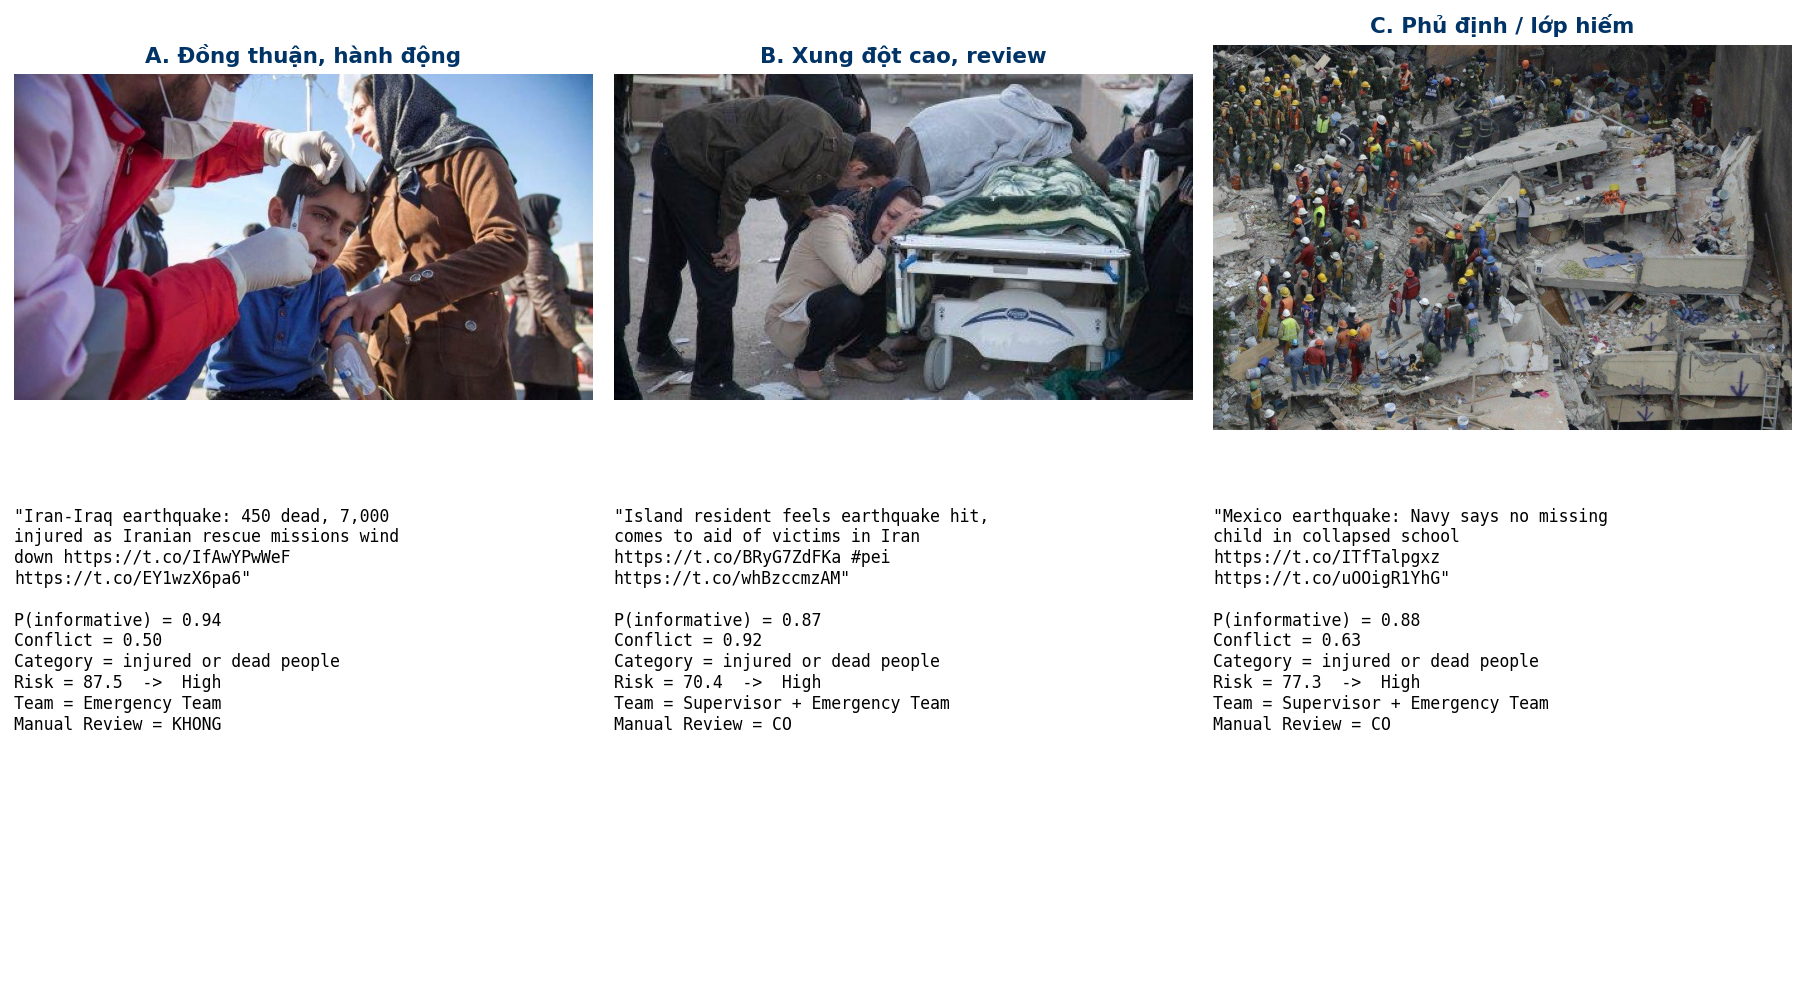
\includegraphics[width=\textwidth]{case_studies.png}
\caption{Ba ca thật từ test. A: tin đồng thuận, Risk 87,5 $\rightarrow$ High,
không cần review. B: xung đột cao (conflict 0,92) nên bật Manual Review dù vẫn
ưu tiên. C: tweet ``no missing child'' -- một câu \emph{phủ định} thật, lớp
missing/found hiếm, hệ thống chuyển review thay vì tin tuyệt đối. Ca C cho thấy
đúng điểm yếu phủ định của TF--IDF đã nêu ở Chương~\ref{chap:mohinh}.}
\label{fig:case-studies}
\end{figure}

\section{Khuyến nghị vận hành}

\begin{enumerate}[leftmargin=*]
  \item \textbf{Dùng hệ thống để sàng lọc, không tự động điều động.}
        Priority và Routing là đề xuất ban đầu; người điều phối xác minh nguồn,
        vị trí và tình trạng hiện trường trước khi phân bổ nguồn lực.
  \item \textbf{Xử lý High trước nhưng vẫn phân tầng trong High.}
        Case injured/missing, có từ khóa khẩn cấp và địa điểm rõ nên được xem
        trước case thiệt hại tài sản.
  \item \textbf{Review song song, không chặn phản ứng khẩn cấp.}
        Khi case High có conflict, Supervisor và đội phản ứng gốc cùng nhận;
        không chờ xác minh xong mới gửi tín hiệu cho Emergency Team.
  \item \textbf{Quản lý công suất Manual Review.}
        Theo dõi số case theo ca trực. Capacity thấp hơn 25\% cần tăng ngưỡng;
        capacity cao hơn có thể hạ ngưỡng sau khi kiểm tra Precision/Recall.
  \item \textbf{Không tự động hóa lớp support rất thấp.}
        Missing/found và vehicle damage cần xác minh bắt buộc cho tới khi có
        thêm dữ liệu và đánh giá ngoài mẫu.
  \item \textbf{Theo dõi drift theo sự kiện.}
        Dùng event filter, so sánh phân bố và metric. Không áp dụng nguyên
        threshold từ dữ liệu năm 2017 cho một thảm họa mới mà không hiệu chỉnh.
  \item \textbf{Phê duyệt Risk policy bằng dữ liệu nghiệp vụ.}
        Cần chuyên gia gán Priority, chi phí bỏ sót, thời gian xử lý và kết quả
        thực tế để kiểm định trọng số Risk Score.
\end{enumerate}

\section{Trả lời tám câu hỏi của bài tập}

\begin{enumerate}[leftmargin=*]
  \item \textbf{Bài toán thực tế mà nhóm giải quyết là gì?}\\
        Trong thảm họa, lượng bài đăng mạng xã hội vượt khả năng đọc thủ công,
        nội dung nhiễu và hai nguồn text--image có thể không đồng nhất. Bài toán
        là chuyển dòng dữ liệu này thành một hàng đợi có cấu trúc để giảm thời
        gian sàng lọc và hỗ trợ điều phối.

  \item \textbf{Ai là người sử dụng hệ thống?}\\
        Người dùng chính là ban điều phối và các Emergency, Relief,
        Infrastructure, Coordination Team. Supervisor xử lý case mâu thuẫn.
        Người dân không trực tiếp nhận quyết định từ model.

  \item \textbf{Hệ thống hỗ trợ những quyết định nào?}\\
        Năm quyết định gồm: bài có đáng chú ý hay không; thuộc nhóm nhu cầu nào;
        Priority Low/Medium/High; đội nào tiếp nhận; và có cần Manual Review hay
        không. Hệ thống đề xuất, con người chịu trách nhiệm quyết định cuối.

  \item \textbf{Dữ liệu nào được sử dụng?}\\
        18.082 cặp tweet--ảnh CrisisMMD v2.0 từ bảy thảm họa năm 2017, gồm nhãn
        informative, tám lớp humanitarian, nhãn riêng text/image và cờ đồng
        thuận. Nhãn informative chính thức được join theo cặp ID; duplicate
        chính xác và gần trùng được kiểm tra trước đánh giá.

  \item \textbf{Dữ liệu được xử lý và phân tích như thế nào?}\\
        Văn bản được làm sạch và biểu diễn bằng TF--IDF 2.000 chiều. Ảnh được
        chuyển thành CLIP embedding 512 chiều với trọng số CLIP giữ nguyên.
        EDA dùng thống kê, K-Means, Apriori, t-SNE và conflict analysis. Sáu
        classifier được so sánh; họ thắng được tune trên dev rồi Late Fusion
        kết hợp xác suất.

  \item \textbf{Kết quả quan trọng nhất là gì?}\\
        Informative fusion đạt Accuracy .6948, F1 .8025, F2 .9045; F2 chỉ hơn
        always-informative .0106. Humanitarian fusion đạt Macro-F1 .4005 so với
        majority .0686. Trên robust test không tune lại, F2 còn .9016 và
        Macro-F1 .3908. Lớp hiếm vẫn là điểm yếu lớn nhất.

  \item \textbf{Hành động nào được đề xuất từ kết quả?}\\
        Dùng Priority Queue, routing theo category, review song song khi
        conflict, bắt buộc xác minh lớp hiếm và hiệu chỉnh ngưỡng theo công suất.
        Giám sát kết quả theo event để phát hiện domain shift.

  \item \textbf{Hạn chế và rủi ro là gì?}\\
        Dữ liệu chỉ từ năm 2017, thiếu GPS và xác minh hiện trường, lớp hiếm rất
        nhỏ, còn tương quan trong cùng event, có duplicate, CLIP không được
        thích nghi riêng cho miền, và Priority không có ground truth. Prototype
        chưa được kiểm thử tải production hoặc tác động thực địa.
\end{enumerate}

\section{Điều đã chứng minh và chưa chứng minh}

\begin{table}[H]\centering\small
\caption{Biên giới của kết luận.}
\begin{tabularx}{\textwidth}{XX}
\toprule
\textbf{Đã có bằng chứng} & \textbf{Chưa có bằng chứng}\\
\midrule
Fusion hơn dummy về nhiều metric và hơn từng nhánh ở humanitarian &
F2 gain khoảng .01 tạo lợi ích vận hành lớn\\
Classifier đã được so sánh và tune chỉ trên dev &
Một cấu hình sẽ tổng quát hóa sang thảm họa chưa thấy\\
Conflict rule có Precision .7532 dưới capacity 25\% &
Manual Review thu hồi được mọi xung đột quan trọng\\
Routing phủ đủ tám category và qua scenario test &
Priority threshold và severity weight là tối ưu thực tế\\
Robustness/CI không đảo ngược kết luận tổng thể &
Lớp missing đủ tin cậy để tự động điều động\\
Dashboard chạy với model và cache đã khóa &
Hệ thống đáp ứng bảo mật, tải và độ trễ production\\
\bottomrule
\end{tabularx}
\end{table}

Giá trị chính của dự án nằm ở sự kết hợp giữa dự báo và quản trị quyết định:
model giảm khối lượng thông tin, còn chính sách minh bạch, capacity constraint,
scenario test và human-in-the-loop giới hạn cách kết quả được sử dụng.

\chapter{Sản phẩm: Dashboard hỗ trợ điều phối}

\section{Vai trò của giao diện trong DSS}

Một DSS chỉ có model nhưng không có giao diện quyết định sẽ khó được sử dụng.
Dashboard là lớp tương tác giữa dữ liệu, mô hình và người điều phối. Nó không
chỉ hiển thị Accuracy; nó phải cho phép người dùng:

\begin{itemize}[leftmargin=*]
  \item quan sát workload và phân bố Priority;
  \item truy vết từ khuyến nghị về xác suất, category và conflict;
  \item lọc theo event, đội nhận và nhu cầu review;
  \item thử một trường hợp mới;
  \item xuất hàng đợi để tiếp tục xử lý.
\end{itemize}

Streamlit là frontend của prototype. Đây là framework Python tạo giao diện web
từ widget, biểu đồ và state; trình duyệt là phía hiển thị, còn mã Python chạy ở
server. Vì vậy dự án không cần thêm React hoặc một frontend riêng để đáp ứng
luồng sử dụng học thuật. Frontend tách rời chỉ cần khi có API độc lập, phân
quyền phức tạp, nhiều người dùng đồng thời hoặc yêu cầu giao diện cao hơn.

\section{Năm trang chức năng}

\begin{description}[leftmargin=3.8cm,style=nextline]
  \item[Overview] Hiển thị số case, Priority, Manual Review, routing team,
        category và phân bố Risk Score. Bộ lọc event giúp quan sát thay đổi
        workload giữa các thảm họa.
  \item[EDA] Trình bày thống kê train-only, phân bố nhãn, K-Means, Apriori,
        kiểm kê ảnh và bất đồng đa phương thức. Trang này giải thích căn cứ
        thiết kế, không dùng test để khám phá.
  \item[Model Evaluation] Hiển thị so sánh sáu model trên dev, tuning,
        baseline, fusion, robust test và metric từng lớp. Người đọc có thể thấy
        cả điểm mạnh lẫn lớp yếu.
  \item[Single-Case Demo] Nhận tweet và ảnh upload. Chế độ text-only cho kết quả
        nhanh; chế độ text+image chạy CLIP rồi toàn bộ fusion--DSS. Kết quả gồm
        xác suất, category, conflict, Risk, Priority, team và action.
  \item[Priority Queue] Cho phép lọc theo Priority, team, event và Manual Review;
        xem chi tiết từng hàng và tải CSV để bàn giao.
\end{description}

\begin{figure}[H]\centering
\begin{subfigure}{0.48\textwidth}
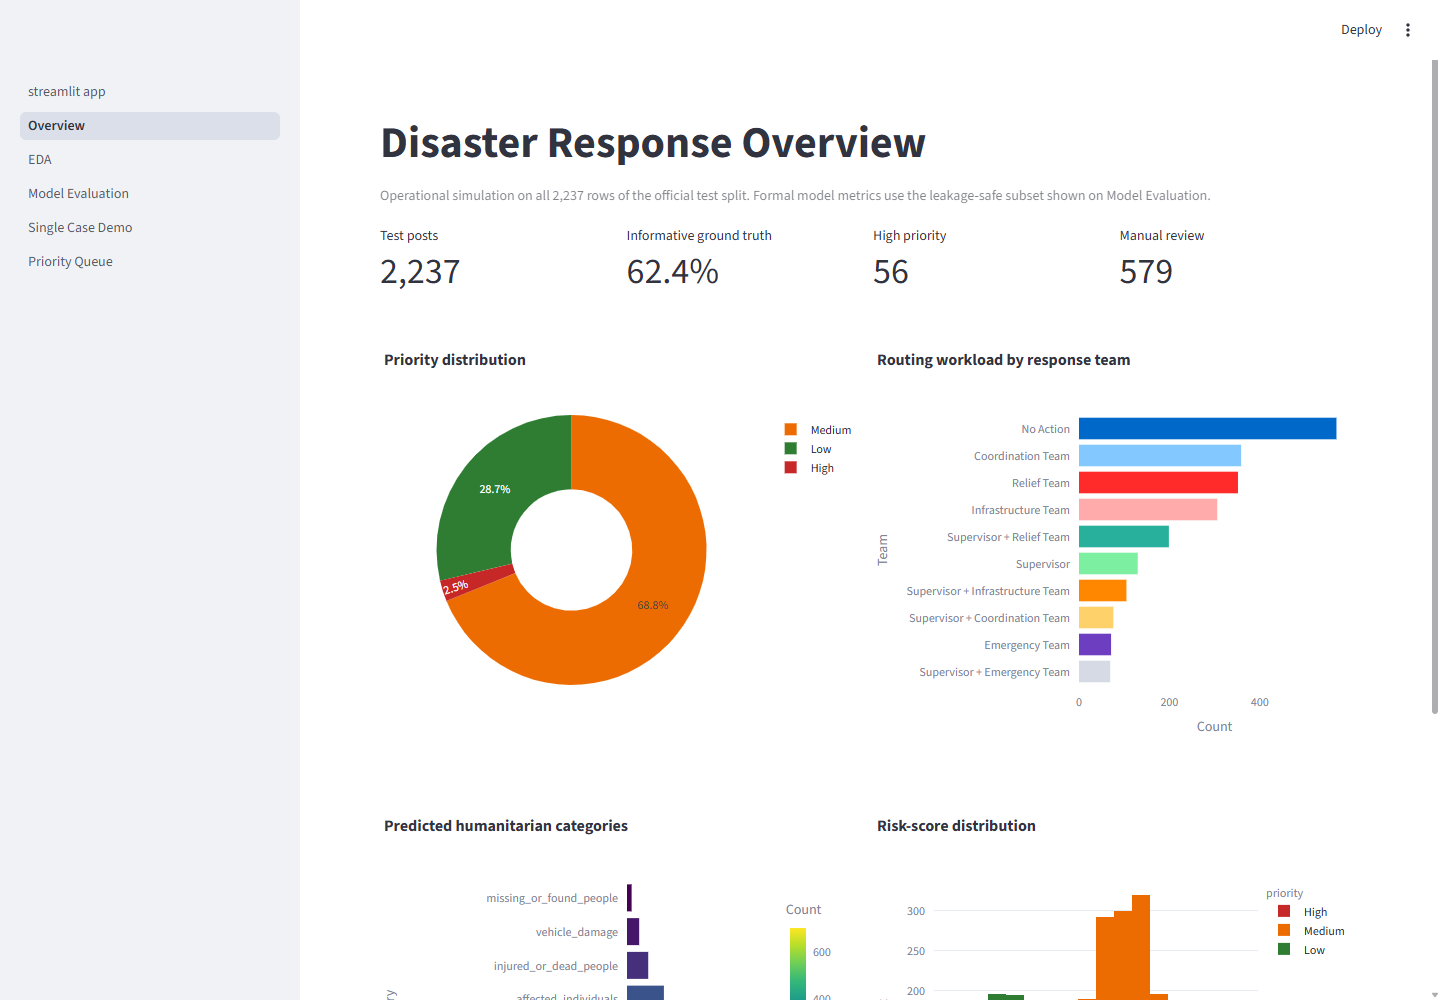
\includegraphics[width=\textwidth]{01_overview_safe.png}
\caption{Overview và workload.}
\end{subfigure}
\begin{subfigure}{0.48\textwidth}
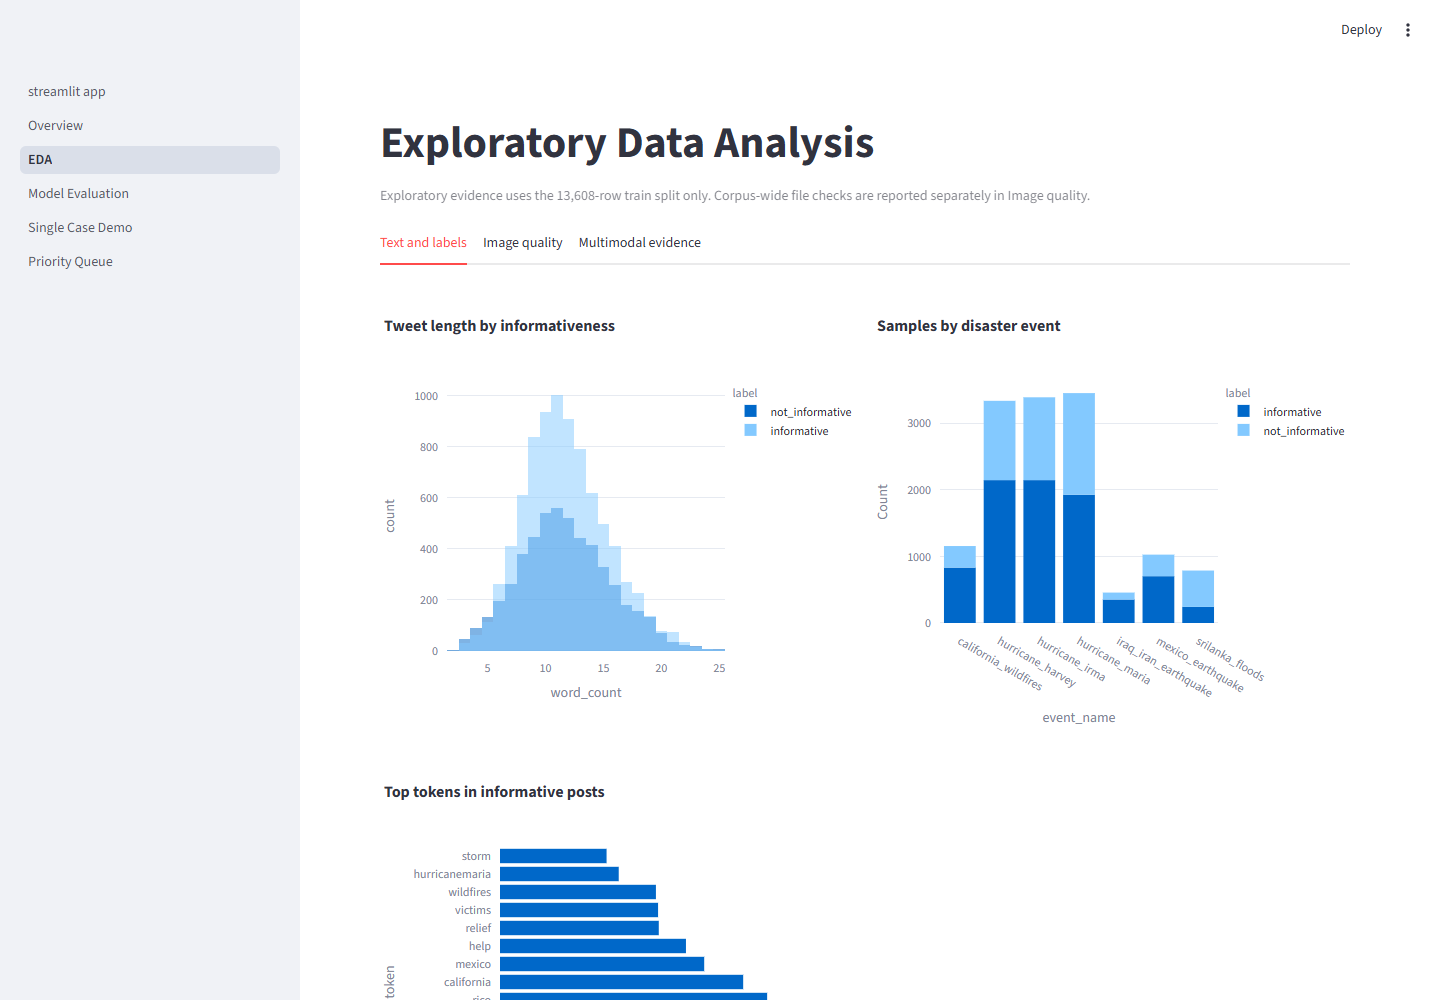
\includegraphics[width=\textwidth]{02_eda_train_only.png}
\caption{EDA train-only.}
\end{subfigure}
\caption{Tổng quan vận hành và căn cứ dữ liệu.}
\end{figure}

\begin{figure}[H]\centering
\begin{subfigure}{0.48\textwidth}
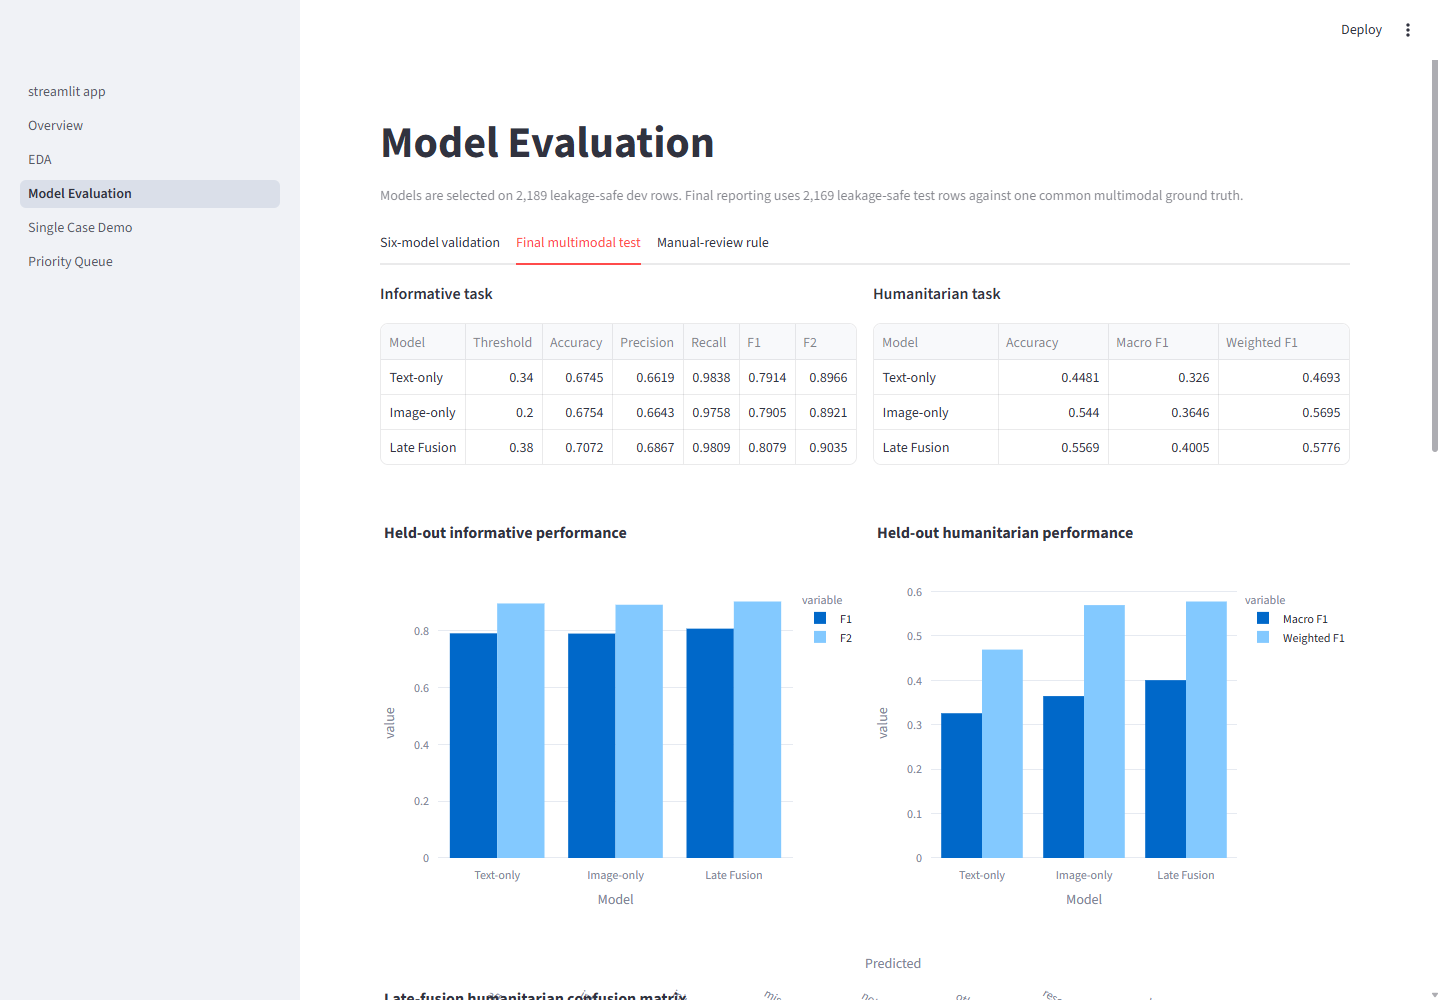
\includegraphics[width=\textwidth]{03_model_fusion_safe.png}
\caption{Đánh giá mô hình.}
\end{subfigure}
\begin{subfigure}{0.48\textwidth}
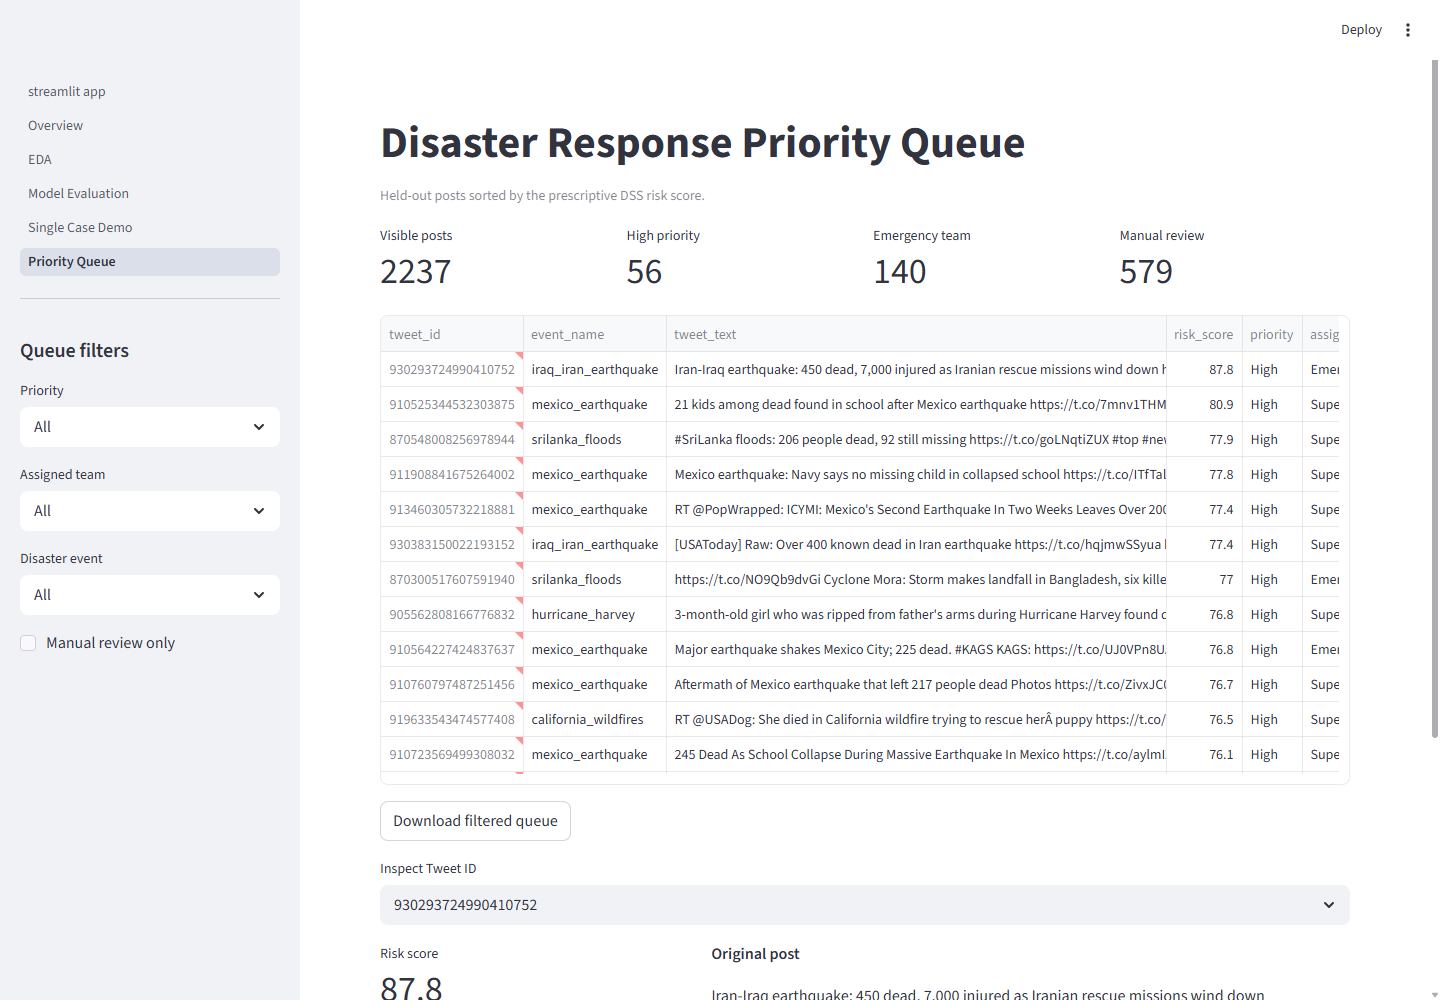
\includegraphics[width=\textwidth]{05_priority_queue_safe.png}
\caption{Priority Queue.}
\end{subfigure}
\caption{Từ bằng chứng mô hình tới hàng đợi quyết định.}
\end{figure}

\section{Kiến trúc dữ liệu của dashboard}

Dashboard không huấn luyện lại model khi người dùng mở trang. Batch test đã
được xử lý thành \code{dashboard\_test\_predictions.csv}, gồm xác suất fusion,
category, Risk Score, Priority, routing và cờ review. Cách cache này:

\begin{itemize}[leftmargin=*]
  \item giảm thời gian tải trang;
  \item bảo đảm biểu đồ dùng đúng model đã khóa;
  \item tách đánh giá hàng loạt khỏi suy luận một trường hợp.
\end{itemize}

Single-Case Demo tải vectorizer và bốn classifier. Model ảnh được lazy-load:
chỉ khi người dùng upload ảnh thì PyTorch/Transformers và CLIP mới được nạp.
Nhờ vậy chế độ text-only khởi động nhanh và cloud không phải tải CLIP ở mọi
trang.

\section{Công nghệ và lý do lựa chọn}

\begin{table}[H]\centering\small
\caption{Vai trò của các công nghệ chính.}
\begin{tabularx}{\textwidth}{p{3.1cm}p{3.3cm}X}
\toprule
\textbf{Công nghệ} & \textbf{Định nghĩa/vai trò} & \textbf{Lý do sử dụng}\\
\midrule
Python & Ngôn ngữ thực thi pipeline & Hệ sinh thái dữ liệu/ML thống nhất, dễ tái lập.\\
pandas/NumPy & Bảng dữ liệu và đại số mảng & Join annotation, audit, cache và tính metric.\\
scikit-learn & Thư viện ML cổ điển & Cung cấp TF--IDF, sáu classifier, metric và API nhất quán.\\
PyTorch + Transformers & Runtime mô hình tiền huấn luyện & Nạp CLIP và chạy forward pass ảnh.\\
Streamlit & Framework web bằng Python & Tạo frontend trực tiếp trên cùng logic dự án.\\
Plotly/Matplotlib & Thư viện trực quan & Biểu đồ tương tác trên app và hình tĩnh cho báo cáo.\\
Jupyter & Notebook thực thi & Lưu code, output và hình EDA/model trong một tài liệu.\\
XeLaTeX & Hệ dàn trang báo cáo & Hỗ trợ tiếng Việt, công thức, bảng và PDF nhất quán.\\
\bottomrule
\end{tabularx}
\end{table}

Việc dùng một stack Python giảm nguy cơ giao diện tính lại metric khác backend.
Đánh đổi là Streamlit không tối ưu cho ứng dụng giao dịch thời gian thực hoặc
UI tùy biến sâu.

\section{Chạy local và triển khai Streamlit Community Cloud}

\subsection{Chạy local đầy đủ}

\begin{verbatim}
pip install -r requirements.txt
streamlit run app/streamlit_app.py
\end{verbatim}

Nếu cần tái tạo toàn bộ dữ liệu, embedding và mô hình:

\begin{verbatim}
python -m scripts.run_all
\end{verbatim}

Lệnh tái tạo đầy đủ cần corpus ảnh CrisisMMD khoảng 1,8 GB và thời gian chạy
CLIP. Khi model/cache đã có, không cần chạy lại pipeline trước khi mở dashboard.

\subsection{Bundle cloud}

Repository cloud chứa:

\begin{itemize}[leftmargin=*]
  \item processed train/test cần cho EDA và dashboard;
  \item vectorizer và bốn classifier đã khóa;
  \item cấu hình fusion và các bảng metric;
  \item mã Streamlit cùng requirements CPU.
\end{itemize}

Raw image corpus và ma trận embedding lớn không được đưa lên Git. Trang EDA đọc
processed CSV. Single-Case Demo nhận ảnh upload; lần suy luận ảnh đầu tiên tải
CLIP nên có cold start, còn text-only dùng ngay các model nhỏ.

Cấu hình deploy:

\begin{center}
\begin{tabular}{ll}
\toprule
Repository & \code{dafiiscoding/ml-dss}\\
Branch & \code{main}\\
Main file & \code{app/streamlit\_app.py}\\
Python & 3.12\\
Secrets & Không yêu cầu\\
\bottomrule
\end{tabular}
\end{center}

Các bước trên được mô tả chi tiết trong \code{docs/DEPLOY\_STREAMLIT.md}.

\section{Kiểm thử giao diện và giới hạn triển khai}

Sáu entrypoint Streamlit gồm trang chính và năm trang chức năng được chạy bằng
AppTest trong môi trường cloud Python 3.12. GitHub Actions kiểm tra bundle,
dependency và text-only inference sau mỗi lần push. Unit test kiểm tra logic
dữ liệu, duplicate mask, tuning, robustness và DSS; integration test chạy một
ảnh thật qua CLIP.

Những kiểm thử này chứng minh app khởi động và luồng chính không phát sinh
exception. Chúng chưa chứng minh khả năng chịu tải nhiều người dùng, bảo mật
upload, phân quyền, lưu audit log hoặc SLA. Nếu triển khai thực tế cần thêm API,
authentication, giới hạn file, quét nội dung, logging, giám sát latency và chính
sách bảo vệ dữ liệu.

\begin{insight}[Phạm vi sản phẩm]
Dashboard là một prototype DSS có frontend hoàn chỉnh cho học tập và trình diễn:
người dùng có thể xem bằng chứng, thử ca mới và thao tác hàng đợi. Nó chưa phải
hệ thống chỉ huy production và không được dùng để tự động điều động nguồn lực.
\end{insight}

\chapter{Kết luận và hướng phát triển}

\section{Kết luận}
Dự án đã thay dữ liệu synthetic bằng CrisisMMD thật, sửa lỗi nhãn informative 2.649 mẫu,
kiểm soát duplicate xuyên split và xây dựng quy trình tái lập từ EDA đến quyết định. Sáu
thuật toán được so sánh trên dev sạch. Informative fusion đạt Accuracy 0,7072, F1 0,8079
và F2 0,9035, nhưng F2 chỉ hơn always-positive baseline 0,0096. Humanitarian fusion đạt
Macro-F1 0,4005 so với majority baseline 0,0686 trên test sạch. Giá trị chính không chỉ
là dự báo nhãn, mà là chuyển kết quả thành hàng đợi, mức ưu
tiên, đội tiếp nhận và cơ chế human-in-the-loop có giới hạn năng lực rõ ràng.

Hậu kiểm loại thêm near-duplicate đã xác minh cho F2 0,9006 và Macro-F1 0,3908 mà không
tune lại. Bootstrap cho thấy F2 gain so với dummy có CI 95\% [0,0032; 0,0161], tức khác
0 theo giả định row-bootstrap nhưng vẫn nhỏ về thực tiễn. Biến động theo event và support
rất thấp ở ba lớp khẩn cấp cho thấy hệ thống phù hợp hỗ trợ sàng lọc, chưa phù hợp tự động
ra quyết định sinh tử.

\section{Hướng phát triển}
\begin{itemize}[leftmargin=*]
  \item Tích hợp NER trích xuất địa danh để định vị người kêu cứu.
  \item Crawl dữ liệu thời gian thực; hiệu chỉnh xác suất (calibration).
  \item Thay TF-IDF bằng embedding ngôn ngữ; tinh chỉnh trọng số fusion theo lớp.
  \item Thu thập ground truth Priority và chi phí xử lý để học/tối ưu policy Risk Score.
  \item Leave-one-event-out hoặc group split theo event để đánh giá domain shift nghiêm ngặt hơn.
\end{itemize}

\appendix
\chapter{Phụ lục}

\section{Khai báo sử dụng công cụ AI}

Theo yêu cầu công khai công cụ hỗ trợ, nhóm có sử dụng Claude và OpenAI Codex
để gợi ý cấu trúc, hỗ trợ rà soát mã nguồn, kiểm thử và biên tập diễn đạt.
Nhóm chịu trách nhiệm lựa chọn phương pháp, chạy chương trình, kiểm tra kết quả
với dữ liệu CrisisMMD, đối chiếu metric và xác nhận nội dung báo cáo. Nội dung
do công cụ sinh ra không được xem là bằng chứng nếu không có kết quả thực thi
hoặc nguồn tham khảo tương ứng.

\section{Bảng tự đánh giá}

\begin{table}[H]\centering\small
\caption{Tự đánh giá theo các nhóm tiêu chí của bài tập.}
\begin{tabularx}{\textwidth}{XrrX}
\toprule
\textbf{Tiêu chí} & \textbf{Tối đa} & \textbf{Tự đánh giá} & \textbf{Căn cứ}\\
\midrule
Hiểu bài toán và quyết định & 15 & 14 & Chương 1--2, stakeholder và năm quyết định\\
Dữ liệu và tiền xử lý & 15 & 15 & Nhãn chính thức, feature engineering, leakage audit\\
EDA và insight & 20 & 19 & Train-only, event, K sweep, Apriori, ảnh, conflict\\
Mô hình và DSS & 20 & 18 & Sáu model, tuning, fusion, robustness, policy test\\
Diễn giải và khuyến nghị & 15 & 14 & Chương 6, capacity, giới hạn bằng chứng\\
Báo cáo và minh chứng & 10 & 9 & PDF, notebook có output, dashboard, metrics\\
Tổ chức nhóm & 5 & 2 & Đã có danh sách; phân công/tỷ lệ cần nhóm xác nhận\\
\midrule
\textbf{Tổng} & \textbf{100} & \textbf{91} & Không tự chấm tối đa ở phần chưa hoàn tất\\
\bottomrule
\end{tabularx}
\end{table}

\section{Cấu hình và siêu tham số chính}

\begin{table}[H]\centering\small
\begin{tabularx}{\textwidth}{p{3.5cm}X}
\toprule
\textbf{Thành phần} & \textbf{Cấu hình đã khóa}\\
\midrule
TF--IDF & 2.000 đặc trưng, word n-gram (1,2), stopword tiếng Anh, \(L_2\).\\
Text informative & Linear SVM \(C=3\), class weight balanced, sigmoid calibration 3-fold.\\
Text humanitarian & Logistic Regression \(C=1\), class weight balanced.\\
Image informative & k-NN \(k=41\), distance weighting, Euclidean trên CLIP normalized.\\
Image humanitarian & Logistic Regression \(C=1\), class weight balanced.\\
Decision Tree & max depth 20 trong vòng so sánh thuật toán.\\
Random Forest & 200 cây, balanced subsample.\\
K-Means & \(K=2,\ldots,12\), \(n\_init=10\); \(K=8\) để đối chiếu taxonomy.\\
Apriori & min support .005, min confidence .25 trên transaction đã lọc.\\
CLIP & \code{openai/clip-vit-base-patch32}, frozen, embedding 512 chiều.\\
Late Fusion & Informative text/image .70/.30, threshold .38; category .55/.45.\\
Manual Review & Conflict threshold .54, capacity dev tối đa 25\%.\\
\bottomrule
\end{tabularx}
\end{table}

\section{Tệp minh chứng và khả năng tái lập}

\begin{itemize}[leftmargin=*]
  \item Notebook đã thực thi:
        \code{notebooks/02\_eda.ipynb} và \code{03\_modeling.ipynb}.
  \item Kiểm tra dữ liệu:
        \code{reports/metrics/data\_quality\_summary.json} và
        \code{data/processed/split\_integrity.csv}.
  \item Tuning và kết quả:
        \code{reports/metrics/*\_tuning.csv},
        \code{tuned\_model\_summary.json} và các bảng fusion.
  \item Robustness:
        canonical/robust comparison, bootstrap, event và class stability trong
        \code{reports/metrics/}.
  \item DSS:
        \code{dss\_scenarios.csv},
        \code{dss\_threshold\_sensitivity.csv}.
  \item Kiểm thử: 41 unit test, 6 Streamlit AppTest và integration ảnh thật.
  \item Mã nguồn:
        \url{https://github.com/dafiiscoding/ml-dss}.
\end{itemize}

\section{Thông tin còn cần nhóm xác nhận}

Tên, MSSV, giảng viên và nhóm đã được điền ở đầu báo cáo. Trước khi nộp chính
thức, nhóm cần phân công các gói công việc và điền tỷ lệ đóng góp thực tế tại
\code{docs/team\_info.json}; tổng tỷ lệ của bốn thành viên cần bằng 100\%.

\begin{thebibliography}{9}
\addcontentsline{toc}{chapter}{Tài liệu tham khảo}

\bibitem{crisismmd2018} Firoj Alam, Ferda Ofli, Muhammad Imran.
\textit{CrisisMMD: Multimodal Twitter Datasets from Natural Disasters}. ICWSM, 2018.
\url{https://crisisnlp.qcri.org/crisismmd}

\bibitem{multimodal2020} Ferda Ofli, Firoj Alam, Muhammad Imran.
\textit{Analysis of Social Media Data using Multimodal Deep Learning for Disaster Response}. ISCRAM, 2020.

\bibitem{clip2021} Alec Radford et al.
\textit{Learning Transferable Visual Models From Natural Language Supervision (CLIP)}. ICML, 2021.

\bibitem{sklearn} Pedregosa et al. \textit{Scikit-learn: Machine Learning in Python}. JMLR, 2011.

\bibitem{mlxtend} Sebastian Raschka. \textit{MLxtend: Providing machine learning and
data science utilities and extensions to Python's scientific computing stack}. JOSS, 2018.

\bibitem{slides} Slide bài giảng và hướng dẫn bài tập nhóm học phần Hệ hỗ trợ quyết định
do TS. Lê Hải Hà cung cấp, học kỳ 2025.2.
\end{thebibliography}

\end{document}
